\documentclass[12pt]{article}
\usepackage[utf8]{inputenc}
\usepackage[french]{babel}
\usepackage[tikz]{bclogo}
\usepackage{geometry}
\usepackage{array}
\usepackage{version}
\usepackage{graphics}
\usepackage{graphicx}
\usepackage{pgfgantt}
\usepackage{url}
\usepackage{enumitem}
\bibliographystyle{alpha}
\usepackage[counterclockwise]{rotating}
\geometry{hmargin=2.5cm,vmargin=1.5cm}

\setlength{\parskip}{1ex plus 2ex minus 1ex}
\newcolumntype{M}[1]{
    >{\raggedright}m{#1}
}

\newenvironment{besoins}
{ \begin{itemize}[topsep=20pt]   }
{ \end{itemize}                  } 

\newcommand{\priority}[1] {
  (\textit{Priorité}:#1)
}
\newcommand{\besoin}[3]{
	\item #1 \priority{#2} #3
}

\title{
 \begin{minipage}\linewidth
        \centering
        Simulation d'algorithmes d'équilibrage de charge dans un environnement distribué 
        \vskip3pt
        \large Memoire final
    \end{minipage}
 }
 
\bibliographystyle{alpha}
\author{Kevin Barreau \and Guillaume Marques \and Corentin Salingue}

\begin{document}

\maketitle

\abstract
Ce document, mémoire final de notre Projet de Programmation, décrit l'ensemble du projet et les algorithmes utilisés. Il contient aussi les besoins fonctionnels et non fonctionnels ainsi que l'architecture du produit final. Enfin, il récapitule point par point le travail effectué ainsi que sa mise en oeuvre. Le document présente les tests effectués et leurs analyses. Enfin, il conclue sur les améliorations possibles du produit.

\newpage


\renewcommand{\contentsname}{Sommaire} 
\tableofcontents

\newpage

\listoffigures

\newpage

\section{Présentation du projet}

Dans le présent document, nous considérons que le lecteur possède des notions en informatique et que chaque mot est défini par son sens commun. Cependant, si un terme qui est utilisé présentant une définition différente que celle admise par tous, nous ne manquerons pas de le préciser et de le définir.

\subsection{Utilisation d'une base de données par un client}

\paragraph{} Une \textit{base de données} est un outil permettant de stocker et récupérer des \textit{données}, qui sont des informations binaires utilisant des structures propres au système de base de données.

\paragraph{} Dans un premier temps, le client se connecte à la base de données.
Le client interagit avec celle-ci en lui envoyant des \textit{requêtes}, messages, dont la forme dépend de la base de données et permettant de stocker, récupérer ou modifier des données.

\paragraph{}Selon les requêtes émises par le client, la base de données lui renvoie des résultats (voir la figure~\ref{fig:bd}).


\begin{figure}[h]
	\centering
		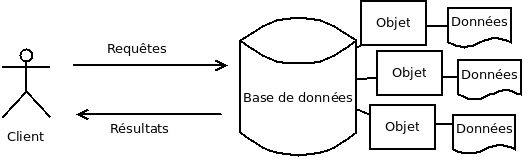
\includegraphics[width=12cm]{bd.png}
	\caption{Interactions client/base de données \label{fig:bd}}
\end{figure}


\paragraph{} On distingue deux types de requêtes :
\begin{itemize}
 \item Les requêtes de \textbf{lecture}: requêtes ne modifiant pas les données contenues dans la base de données.
 Il s'agit de récupérer des objets contenus dans la base de données.
 
 \item Les requêtes d' \textbf{écriture} : requêtes modifiant les données contenues dans la base de données.
\end{itemize}

\paragraph{} Le client peut être une personne physique ou un logiciel. Dans notre cas, il s'agit d'un logiciel permettant l'importation de fichiers contenant des requêtes ou de générer des requêtes pseudo-aléatoirement.


\subsection{Base de données distribuée}

\paragraph{} La base de données utilisée par le client est plus précisément une base de données dite \textit{distribuée}. Le client ne voit pas de différence, lorsqu'il l'utilise, entre une base de données classique et une base de données distribuée. On dit qu'une base de données est distribuée lorsque les données qu'elle stocke sont réparties sur plusieurs machines ou emplacements physiques, appelés \textit{noeuds}. Les noeuds sont capables de communiquer entre eux afin de s'échanger des informations.

\paragraph{} On peut rassembler des noeuds pour former un \textit{data center}. Un rassemblement de data center correspond à un \textit{cluster} (voir la figure~\ref{fig:distributed_database}). Dans ce projet, nous nous intéressons seulement au cas où un cluster est composé d'un seul data center.

\paragraph{} La base de données va stocker les données sous forme d'\textit{objets}. Un \textit{objet} est composé d'une clé d'identification appelée \textit{token} et d'un ensemble de \textit{données}.

\paragraph{} En positionnant les noeuds suivant leur token, on obtient alors une forme d'anneau (ou de \textit{ring}), qui est donc la forme d'un data center.

\paragraph{} Pour savoir quel noeud doit stocker quelle donnée, on utilise une méthode de \textit{partitionnement}. Cette méthode se base sur les \textit{tokens}. Chaque noeud a un token qui lui est attribué. Un noeud prend en charge des objets dont le token est compris entre celui que le noeud possède et celui de son "prédécesseur" (si on imagine un anneau orienté dans le sens du plus petit au plus grand token, sauf pour les extrêmes) dans l'anneau (voir la figure~\ref{fig:partitionning}). Ainsi dans cet exemple, le noeud 2 a le token 25 qui lui est attribué. Il s'occupe donc des objets dont le token est compris entre 25 et 0 (qui est le token le plus grand dans ses prédécesseurs). On parle alors de l'\textit{intervalle} de tokens dont s'occupe le noeud.

\paragraph{} Afin de garantir une meilleure disponibilité, chaque objet possède des copies, appelées \textit{réplicas}, disposées sur d'autres noeuds que le noeud initial (le noeud qui s'occupe du token de cet objet). La méthode pour choisir l'emplacement des copies d'un objet est variable. C'est ce que l'on appelle la \textit{stratégie de réplication}, qui est abordée plus loin dans ce document.

\subsection{Gestion des requêtes dans la base de données distribuée}
\subsubsection{Requêtes de lecture}

\paragraph{} Il est possible de réaliser des requêtes de lecture sur un objet, ce qui consiste à vouloir récupérer une donnée contenue dans un objet. Pour expliquer le cheminement d'une requête de lecture dans la base de données, nous allons prendre un exemple (voir la figure~\ref{fig:request}).

\paragraph{} Un client réalise une requête de lecture R. Il envoie la requête à n'importe quel noeud du réseau. On appelle alors ce noeud : le noeud \textit{coordinateur} pour cette requête. Ce noeud ne contient pas forcément l'objet de la requête, mais il va faire la liaison entre le réseau et le client.

\paragraph{} Le noeud coordinateur va avoir cette requête dans une file d'attente dédiée aux requêtes des clients. Il les traite les unes à la suite des autres. Lorsque le noeud commence à traiter cette requête, il va d'abord identifier les noeuds responsables de l'objet de la requête. Cela inclut le noeud possédant l'objet \textit{original} (dont le token est géré par ce noeud) ainsi que les noeuds possédant un réplica. Cette étape exige une connaissance complète du réseau sur chaque noeud et une connaissance de la stratégie de réplication mise en place.

\paragraph{} Dès que les noeuds sont identifiés, le noeud coordinateur leur envoie un message pour traiter la requête de lecture (les flèches rouges sur le schéma entre le noeud coordinateur et les autres noeuds). Ce message est mis dans la file d'attente des requêtes de lecture de ces noeuds.

\paragraph{} A un moment, l'un des noeuds qui possède cette requête dans sa file d'attente va la défiler et la traiter. Ce noeud s'\textit{affecte} la requête. Il avertit les autres noeuds possédant cette même requête dans leur file d'attente (c.à.d tous les autres noeuds possédant une copie de l'objet de la requête) qu'ils n'auront pas besoin de la traiter, et qu'ils peuvent la supprimer de leur file d'attente (les flèches oranges sur le schéma). Si la requête à supprimer est déjà en cours d'exécution, on la laisse se dérouler normalement. Le noeud qui s'est affecté la requête la traite et renvoie le résultat au noeud coordinateur, qui peut transmettre le résultat obtenu au client (les flèches vertes sur le schéma).

\subsubsection{Requêtes d'écriture}

\paragraph{} Il est possible de réaliser des requêtes d'écriture d'un objet, ce qui consiste à stocker des données dans la base de données, sous forme d'objet.  Pour expliquer le cheminement d'une requête d'écriture dans la base de données, nous allons prendre un exemple (voir la figure~\ref{fig:write_request}). Le cheminement est plus simple que pour une requête de lecture car il n'y a pas le mécanisme d'affectation.

\paragraph{} Un client réalise une requête d'écriture R. Il envoie la requête à n'importe quel noeud du réseau. On appelle alors ce noeud le noeud \textit{coordinateur} pour cette requête. Ce noeud n'est pas forcément celui qui va stocker les données, mais il va faire la liaison entre le réseau et le client.

\paragraph{} Le noeud coordinateur va avoir cette requête dans une file d'attente dédiée aux requêtes des clients. Il les traite les unes à la suite des autres. Lorsque le noeud commence à traiter cette requête, il va d'abord identifier les noeuds responsables de l'objet de la requête. Cela inclut le noeud qui se charge de l'objet \textit{original} (dont le token est géré par ce noeud) ainsi que les noeuds devant posséder un réplica. Cette étape exige une connaissance complète du réseau sur chaque noeud et une connaissance de la stratégie de réplication mise en place.

\paragraph{} Dès que les noeuds sont identifiés, le noeud coordinateur leur envoie un message à tous pour traiter la requête d'écriture (les flèches rouges sur le schéma entre le noeud coordinateur et les autres noeuds). Ce message est mis dans la file d'attente des requêtes d'écriture de ces noeuds.

\paragraph{} Tous les noeuds recevant le message vont alors stocker les données envoyées par la requête. Le noeud coordinateur peut demander un certain nombre de messages de retour pour s'assurer que les requêtes d'écritures se sont bien déroulées. Dans l'exemple, le noeud coordinateur demande \textbf{1} retour. L'un des messages envoyés aux noeuds contiendra donc une demande d'un message de retour pour confirmer que l'écriture s'est bien passée (la flèche verte entre les noeuds sur le schéma). Dès que le noeud coordinateur reçoit le message, il indique au client que sa requête s'est terminée et bien passée.

\subsection{Stockage des données}

\paragraph{} Chaque base de données possède sa propre manière de stocker les données dans un espace de stockage. Pour le projet, la méthode de stockage n'est pas un problème sur lequel nous allons travailler. La seule contrainte imposée pour la base de données est qu'elle stocke les données sous la forme d'objet. C'est à dire qu'un objet est identifiable par son token, une clé d'identification générée le plus souvent par une fonction de hachage.

\paragraph{} Le token est généré par la base de donnée à partir de la \textit{clé primaire} d'une table. Une clé primaire est, comme le token, une donnée permettant d'identifier un objet. Sauf que que la clé primaire est une donnée choisit par le client. Elle peut être un entier, une chaîne de caractères, toutes les représentations possibles d'une donnée au sein de la base de données (voir la figure~\ref{fig:token}).

\subsection{Protocoles de réaffectation des requêtes de lecture}

\paragraph{} Lorsqu'une requête de lecture est envoyée par un client, on a vu précédemment que cette requête était transmise à tous les noeuds possédant une copie de l'objet à lire. Si un nombre important de requêtes de lecture arrivent en même temps, les files d'attentes dans les noeuds pour les requêtes de lecture vont commencer à se remplir plus vite que les requêtes ne sont traitées. Le nombre de requêtes dans une file d'attente est appelée la \textit{charge}. Les charges des files d'attentes ne seront pas forcément uniformes entre les noeuds, certains pouvant avoir plus de requêtes à traiter que d'autre.

\paragraph{} C'est pourquoi on met en place un système de \textit{réaffectation} des requêtes de lecture, afin de rééquilibrer la charge des noeuds. La réaffectation consiste, après chaque modification locale (une modification locale sera le traitement d'une requête de lecture ou de suppression dans notre cas, mais on peut imaginer d'autres moments aussi), à enclencher un processus permettant de décider de l'affectation des requêtes suivant l'état actuel du réseau. Le nombre de requêtes affectées (donc assignées à ce noeud et avec un message de suppression pour ces requêtes envoyé aux autres noeuds) est appelé la \textit{charge effective}. Une requête affectée ne peut pas être supprimée.

\paragraph{} Les algorithmes de réaffectation à implémenter, \textbf{SLVO} et \textbf{AverageDegree}, ont un comportement similaire qui se base sur la connaissance des charges de chaque noeud du réseau. L'algorithme consiste à comparer, pour tous les noeuds, sa propre charge par rapport à une certaine valeur.

\paragraph{} Pour SLVO, la valeur est la charge minimale sur le réseau. Pour AverageDegree, la valeur est la charge moyenne sur le réseau.

\paragraph{} Si la valeur est inférieure ou égale (strictement égale dans le cas de SLVO), alors le noeud s'affecte toutes les requêtes de sa file d'attente et avertit tous les autres noeuds. Les noeuds possédant les requêtes qui ont été affectées les suppriment de leur file d'attente, modifiant ainsi leur charge (voir la figure~\ref{fig:reaffectation} pour un exemple avec SLVO).

\subsection{Gestion de la popularité des objets}

\paragraph{} Pour mieux équilibrer la charge du réseau, nous nous intéressons à la \textit{popularité} des objets. En effet, plus un objet va recevoir de requêtes, plus il sera populaire et occasionnera une grande charge pour les noeuds qui s'en occupent. Afin de répartir cette charge, il faudra alors augmenter ou diminuer le nombre de réplicas. Si un objet est populaire, il suffira de créer de nouveaux réplicas, ce qui permettra d'envoyer une partie de la charge sur d'autres noeuds. A l'inverse, si un objet n'est pas populaire, diminuer le nombre de copies fera gagner de l'espace mémoire et du temps (quand on a besoin de contacter tous les noeuds qui gèrent un objet, le nombre de noeuds influe sur le temps nécessaire à réaliser l'action...).

\paragraph{} Il y a plusieurs méthodes pour calculer la popularité des objets durant un intervalle de temps $T$ défini par l'utilisateur :

\begin{itemize}
    \item La première consiste à ce que chaque noeud possède un vecteur de la taille du nombre d'objets dont il a la gestion. A chaque nouvelle requête, la case de l'objet est incrémentée. Au début de chaque période $T$, les noeuds envoient la popularité aux autres noeuds et décident du nombre de copies à faire.
    \item La seconde méthode est une variante visant à réduire la taille du vecteur d'objets et est défini par le Space-Saving Algorithm \cite{SpaceSaving}. On choisit un vecteur de la taille du nombre de noeuds du réseau qui contient des structures de la forme \textit{( identifiant de l'objet ; nombre de requête )}. Soit $n$ le nombre de noeuds dans le reseau, l'algorithme permet de connaitre les $n$ objets les plus populaires. \newline
          \newline
          Soit une requête sur un objet $o$.\newline
          Si $o$ est présent dans le vecteur, on augmente son nombre de requêtes de 1. \newline
          Si $o$ n'est pas présent dans le vecteur et qu'il reste de la place (la taille du vecteur est inférieure à $n$), on l'ajoute au vecteur avec un nombre de requête de 1. \newline
          Si $o$ n'est pas présent et que le vecteur est plein, on cherche l'endroit qui contient l'objet le moins populaire du vecteur et on le remplace par $o$. Cependant, on garde la popularité de l'ancien objet et on l'incrèmente de 1. \newline
          Il est possible de consulter le pseudo code sur la figure~\ref{fig:codeSpaceSaving}
\end{itemize}

\paragraph{}Soient les paramètres suivants : \newline
            $r$ = Nombre de requêtes total effectuées durant l'intervalle de temps $T$; \newline
            $n$ = Nombre de noeuds dans le réseau; \newline
            $p$ = Popularité d'un objet; \newline
            $k$ = Nombre de copies de l'objet.

\paragraph{} On augmente le nombre de copies d'un objet quand la formule suivante est respectée :  $ 2 \times \frac{r}{n} \geq \frac{p}{k} $

\paragraph{} On diminue le nombre de copies d'un objet quand la formule suivante est respectée : $ \frac{r}{2n} \leq \frac{p}{k} $

\subsection{Gestion des copies d'un objet}

\paragraph{} Une \textit{fonction de hachage} est une fonction mathématique qui possède les propriétés suivantes :
\begin{itemize}
    \item Ensemble d'entrée : une clé primaire ;
    \item Ensemble d'arrivée : Un entier ;
\end{itemize}
On lui associe souvent d'autres propriétés pour équilibrer la répartition des données (cf paragraphe suivant).

\paragraph{} Pour fabriquer un token, qui sert à placer les données sur le réseau, une clé primaire est hachée avec une fonction de hachage. Nous obtenons une valeur (ici un entier). Chaque noeud du réseau est responsable d'un intervalle d'entiers de l'ensemble des valeurs du domaine. Avec une bonne fonction de hachage, les hash des clés primaires seront distribués uniformément dans l'ensemble des entiers.

\paragraph{} Placer les copies sur le même noeud revient à n'avoir théoriquement l'équivalent d'aucune copie puisque la charge reste sur le même noeud. Il existe plusieurs stratégies de placement de copies des données et nous n'en développerons que deux ici. La première permet de comprendre les mécanismes de base d'une stratégie de placement. La seconde décrit celle que nous allons développer.

\paragraph{} On le rappelle, chaque noeud possède la gestion d'un intervalle de \textit{tokens}. La base de données se base sur des intervalles d'entiers. Si on organise ces noeuds selon l'ordre croissant des intervalles, on obtient un cercle. \newline
La plus simple stratégie consiste à prendre les noeuds qui suivent sur ce cercle. Prenons comme exemple la figure~\ref{fig:replication}. Nous souhaitons stocker une donnée. La fonction de hachage de la clé primaire de notre donnée retourne 123. La donnée originale est donc placée sur le noeud 2. \newline
De plus, notre stratégie va créer des réplicas qu'elle disposera sur les noeuds suivants. Ici, on a décidé que 3 réplicas suffisaient, les copies sont donc placées sur les noeuds 3, 4 et 5.

\paragraph{} La seconde consiste à utiliser les fonctions de hachage. En effet, dans la stratégie précédente, une seule fonction de hachage était définie pour placer la donnée et la position des réplicas était ensuite déterminée à partir de l'emplacement de la première. \newline
Supposons qu'on a au maximum $n$ fois la donnée présente dans le réseau (c'est à dire $n$ = nombre de copies d'une donnée + 1 pour le placement initial). Nous avons besoin de $n$ fonctions de hachage, toutes numérotées de $0$ à $n-1$. La fonction de hachage numéro 0 sert à placer la donnée. La fonction numéro 1 sert à placer le premier réplica, la fonction numéro 2 sert à placer le second réplica et ainsi de suite...

\subsection{Visualisation des statistiques de fonctionnement de la base de données distribuée}

\paragraph{} Le but est de visualiser les statistiques de fonctionnement de la base de données pour permettre une comparaison de l'efficacité des algorithmes d'équilibrage de charge.

\paragraph{} On souhaite récupérer:
\begin{itemize}
 \item la charge effective de chaque noeud ou taille de la file d'attente des requêtes de lecture.
 \item une représentation de la file d'attente des requêtes de lecture
 \item la popularité de chaque objet
 \item la requête en cours de traitement
\end{itemize}

\begin{figure}[h]
	\centering
		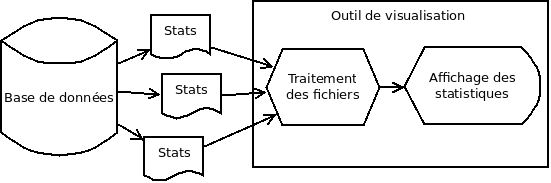
\includegraphics[width=12cm]{visu.png}
	\caption{Processus pour la visualisation des statistiques \label{fig:visu}}
\end{figure}

\paragraph{} On enregistre les statistiques de fonctionnement de la base de données distribuée dans des fichiers. Un outil de visualisation traite ces fichiers et affiche ensuite les statistiques (voir la figure~\ref{fig:visu}).

\newpage
\subsection{Pour en savoir plus...}
Présentations par d'autres auteurs sur le projet :

\paragraph{Système distribué}

\begin{itemize}
\item Le livre \cite{Ozsu2011} apporte les principes sur les bases de données distribuée.

\end{itemize}

\paragraph{Algorithmes d'équilibrage de charges}

\begin{itemize}
\item L'article \cite{BalancedAlloc99} met en exergue des algorithmes d'équilibrage, sources d'inspiration pour les clients dans l'élaboration de leurs algorithmes.

\item Le papier \cite{RandomChoices05}, de là même manière que le précédent, s'intéresse de plus près à des algorithmes d'allocation aléatoire.

\item L'article \cite{LoadBalancingPeertoPeer14} est aussi important car il traite des algorithmes d'équilibrage des charges dans un réseau pair à pair.

\end{itemize}

\paragraph{Cassandra}

\begin{itemize}
\item Le livre \cite{Hewitt2010} renseigne sur la compréhension du fonctionnement de Cassandra, ainsi que les structures particulières de ce système de base de données.

\item Le lien \cite{ApacheCassandra09} permet d'accéder à l'ensemble de la documentation technique et au dépôt des sources de la base de données Cassandra.

\item Le papier \cite{FacebookCassandra09} apporte les explications des créateurs de Cassandra.

\item Le lien \cite{DSDocCassandra15} possède la documentation la plus complète sur la dernière version de Cassandra, et sur les manières de l'utiliser.
Les nombreux exemples et les approfondissements sont des points d'appuis importants pour le projet.

\end{itemize}

\paragraph{Visualisation}

\begin{itemize}
\item Le lien \cite{DSOpsCenter14} est intéressant pour le projet car il apporte un logiciel capable de montrer graphiquement des statistiques sur une base de données Cassandra opérationnelle
Il peut être utilisé dans le projet, ou apporté des pistes pour la visualisation des données.

\item L'article \cite{Tulip12} s'intéresse à un logiciel de représentation de graphe développé au Labri.
La proximité des créateurs peut apporter une solution viable.
\end{itemize} 



\newpage

\section{Ordonnancement des besoins}

\paragraph{} Nous avons dégagé une liste de besoins fonctionnels et non-fonctionnels. 
Pour mieux les comparer, nous les avons ordonnés en fonction de leur priorité.

\paragraph{} La priorité est un indicateur de l'ordre dans lequel nous devrons implémenter les fonctionnalités afin de satisfaire les besoins du client.

\paragraph{}
\begin{tabular}{| l | M{12cm} |}
    \hline
    Valeur & Signification \tabularnewline
    \hline
    1 & Priorité haute \tabularnewline
    \hline
    2 & Priorité moyenne  \tabularnewline
    \hline
    3 & Priorité faible  \tabularnewline
    \hline
 \end{tabular}


\newpage

\section{Besoins fonctionnels}

\subsection{Communication entre les noeuds}

\paragraph{} Tous les besoins concernent un seul noeud. Tous les noeuds du réseau doivent répondre à ces besoins.

\begin{besoins}
\besoin{Envoyer les informations du noeud à n'importe quel autre noeud}{1}
\besoin{Recevoir les informations provenant d'un autre noeud}{1}
\besoin{Stocker les informations de tous les noeuds du réseau}{1}{
Cela concerne tous les noeuds, y compris soi-même.
}
\end{besoins}

\paragraph{} Les informations d'un noeud doivent permettre d'envoyer un message à ce dernier.



\subsection{Gestion des requêtes}

\paragraph{} Tous les besoins concernent un seul noeud. Tous les noeuds du réseau doivent répondre à ces besoins.


\subsubsection{Requêtes client}

\begin{besoins}
\besoin{Créer une file d'attente des requêtes client}{1}
\besoin{Ajouter une requête à la file d'attente des requêtes client}{1}
\besoin{Défiler une requête de la file d'attente des requêtes client}{1}
\besoin{Traiter une requête client}{1}
\end{besoins}

\begin{besoins}
\besoin{Identifier les noeuds responsables d'un objet}{1}{
Cela nécessite de connaitre plusieurs informations :
\begin{itemize}[noitemsep]
	\item la stratégie de réplication
	\item la token de chaque noeud
	\item le nombre de copie de chaque objet
\end{itemize}
}
\end{besoins}

\begin{besoins}
\besoin{Créer une requête de lecture}{1}{
Les requêtes de lecture doivent être identifiable, ceci afin de pouvoir les supprimer. Il faut donc générer un identifiant pour chaque requête de lecture lors de sa création.
}
\besoin{Envoyer une requête de lecture}{1}
\besoin{Créer une requête d'écriture}{1}
\besoin{Envoyer une requête d'écriture}{1}
\end{besoins}


\subsubsection{Requêtes de lecture}

\begin{besoins}
\besoin{Créer une file d'attente des requêtes de lecture}{1}
\besoin{Recevoir une requête de lecture}{1}
\besoin{Ajouter une requête à la file d'attente des requêtes de lecture}{1}
\besoin{Supprimer une requête de la file d'attente des requêtes de lecture}{1}
\besoin{Défiler une requête de la file d'attente des requêtes de lecture}{1}
\besoin{Traiter une requête de lecture}{1}
\end{besoins}

\begin{besoins}
\besoin{Créer un message de suppression de requête de lecture}{1}
\besoin{Envoyer un message de suppression de requête de lecture}{1}
\besoin{Recevoir un message de suppression de requête de lecture}{1}
\besoin{Traiter un message de suppression de requête de lecture}{1}
\end{besoins}

\begin{besoins}
\besoin{Créer un message de résultat}{1}
\besoin{Envoyer un message de résultat au noeud coordinateur}{1}
\besoin{Recevoir un message de résultat}{1}
\besoin{Transmettre un message de résultat au client}{1}
\end{besoins}


\subsubsection{Requêtes d'écriture}

\begin{besoins}
\besoin{Créer une file d'attente des requêtes d'écriture}{1}
\besoin{Recevoir une requête d'écriture}{1}
\besoin{Ajouter une requête à la file d'attente des requêtes d'écriture}{1}
\besoin{Défiler une requête de la file d'attente des requêtes d'écriture}{1}
\besoin{Traiter une requête d'écriture}{1}
\end{besoins}

\begin{besoins}
\besoin{Créer un message de résultat}{1}
\besoin{Envoyer un message de résultat au noeud coordinateur}{1}
\besoin{Recevoir un message de résultat}{1}
\besoin{Transmettre un message de résultat au client}{1}
\end{besoins}



\subsection{Réaffectation des requêtes de lecture}

\paragraph{} Les besoins sur la réaffectation des requêtes de lecture se recoupent avec ceux de gestion des requêtes de lecture en ce qui concerne les messages envoyés entre les noeuds.

\begin{besoins}
\besoin{Connaître la charge des files d'attentes de requêtes de lecture de chaque noeud du réseau}{1}{Cette information fait partie des informations de chaque noeud, communiqué entre eux comme vu précédemment dans la partie \textit{Communication entre les noeuds}.}
\besoin{Définir un protocole de réaffectation}{1}
\besoin{Modifier le protocole de réaffectation par une configuration}{3}{La configuration est accessible par l'utilisateur, et le protocole de réaffectation doit être la même pour tous les noeuds du réseau}
\besoin{Exécuter le code d'un protocole de réaffectation défini}{1}
\end{besoins}


\subsection{Gestion d'un réseau}

\subsubsection{Popularité d'un objet}

\paragraph{Stockage de la popularité}

\paragraph{} Tous les besoins concernent un seul noeud. Tous les noeuds du réseau doivent répondre à ces besoins.

\begin{besoins}
        \besoin{Créer un vecteur d'entiers compatabilisant le nombre de requêtes}{1}
        \besoin{Augmenter la taille du vecteur}{1} dans le cas où on a l'algorithme qui calcule la popularité de tous les objets
        \besoin{Créer un identifiant permettant de relier la popularité à un objet}{1}
\end{besoins}

\paragraph{Calcul de la popularité}

\paragraph{} Tous les besoins concernent un seul noeud. Tous les noeuds du réseau doivent répondre à ces besoins.

\begin{besoins}
        \besoin{Incrémenter la popularité de l'objet requêté dans le vecteur à chaque requête sur celui-ci}{1}
\end{besoins}

\paragraph{Communication de la popularité}

\paragraph{} Tous les besoins concernent un seul noeud. Tous les noeuds du réseau doivent répondre à ces besoins.

\begin{besoins}
        \besoin{Identifier le noeud responsable d'un objet}{1}
        \besoin{Créer un message de popularité}{1}
        \besoin{Envoyer un message de popularité au noeud responsable de l'objet}{1}
        \besoin{Recevoir un message de popularité}{1}
        \besoin{Traiter un message de popularité (cf paragraphe suivant)}{1}
\end{besoins}

\paragraph{Traitement d'un message de popularité}

\paragraph{} Tous les besoins concernent un seul noeud. Tous les noeuds du réseau doivent répondre à ces besoins.

\begin{besoins}
        \besoin{Stocker la popularité du message dans le vecteur du noeud traitant le message}{1}
        \besoin{Vérifier avoir reçu tous les messages concernant les objets dont le noeud a la gestion}{1}
        \besoin{Décider de créer ou non de nouveau réplicas}{1}
        \besoin{Décider de supprimer ou non des réplicas}{1}
        \besoin{Réinitialiser le vecteur après la création des nouveaux objets les plus populaires}{1}
\end{besoins}

\subsubsection{Réplication d'un objet}

\paragraph{} Tous les besoins concernent un seul noeud. Tous les noeuds du réseau doivent répondre à ces besoins.

\begin{besoins}
        \besoin{Créer une nouvelle stratégie de réplication}{1}
        \besoin{Permettre la définition par l'utilisateur de fonctions de hachage et leur ordre d'utilisation}{1}
        \besoin{Stocker chaque fonction de hachage et son ordre}{1}
        \besoin{Définir un ordre dans les réplicas}{1}
        \besoin{Utiliser la première fonction de hachage pour placer le premier réplica}{1} la seconde pour le second, et ainsi de suite...
        \besoin{Retrouver les réplicas en fonction des fonctions de hachage}{1}
\end{besoins}

\subsection{Application cliente}

\subsubsection{Intéractions avec Cassandra}


\begin{besoins}
  	\besoin{Se connecter à Cassandra}{1}
  	\besoin{Se déconnecter de Cassandra}{1}
\end{besoins}
 

\subsubsection{Initialisation des données}

\paragraph{} L'initialisation des données consiste à créer un Keyspace et à enregistrer des données dans celui-ci.

\begin{besoins}
	\besoin{Créer un Keyspace}{1}
	\besoin{Importer des données}{1}
	\besoin{Initialiser les données}{1} Si les données sont modifiées, le client doit pouvoir les initialiser pour revenir aux données d'origine.
\end{besoins}

\subsubsection{Gestion de requêtes}

\paragraph{} Pour tester la validité des algorithmes, l'application devra posséder une fonction de génération de requêtes. 
Si l'utilisateur ne détient pas de suites de requêtes prêtes, il pourra demander à l'application d'en créer pour lui. 
L'application, ne connaissant pas la nature des données, ne pourra qu'effectuer un nombre restreint de requêtes différentes. 
Elle pourra par exemple, compter le nombre de données sauvegardées, chercher si une donnée existe réellement, mais ne pourra pas en modifier une.

\begin{besoins}
  	\besoin{Récupérer le nom des tables}{1} Afin de pouvoir générer des requêtes, nous devons connaître le nom des tables contenues dans un keyspace.
	\besoin{Générer un jeu de données pseudo-aléatoirement}{2} Il s'agit de créer une fonction $f$, qui aura pour ensemble des antécédents des suites de caractères alpha-numériques (par exemple: 5832fg4gh52 ) et pour image un jeu de données.
	\besoin{Importer un jeu de requêtes}{1} L'utilisateur peut importer son propre jeu de requêtes.
\end{besoins}


\subsection{Visualisation des données}

\paragraph{} Afin de suivre l'évolution des charges de chaque noeud lors de l'exécution des algorithmes, on enregistre les données locales de chaque noeud à chaque modifications de celles-ci.

\subsubsection{Enregistrement des données}

\paragraph{Ecriture dans un fichier} Lorsque les données locales d'un noeud sont modifiées, on les enregistre dans un fichier.
L'écriture est de la forme \texttt{itération de l'algorithme; identifiant du noeud; charge du noeud;}

\subsubsection{Affichage des données}

\paragraph{Définition} Un \textit{graphe} est un ensemble de points appelés \textit{sommets}, dont certaines paires sont directement reliées par un (ou plusieurs) lien(s) appelé(s) \textit{arêtes} \cite{graphe}. 

\paragraph{Noeuds} L'application doit permettre la représentation de chaque noeud par un sommet.

\paragraph{Analyse syntaxique} Lors de l'éxecution d'un algorithme, la charge de chaque noeud est enregistrée dans un fichier.
Un analyseur syntaxique (un programme qui possède des règles et qui agit sur un fichier donné en entrée selon celles-ci) découpe chaque ligne du fichier pour récupérer le moment auquel a été enregistrée l'information (\texttt{itération de l'algorithme}),
le noeud concerné ( \texttt{ identifiant du noeud} ) et la charge de ce noeud à ce moment ( \texttt{charge du noeud} ).

\paragraph{Charge des noeuds} A chaque sommet est associée une valeur correspondant à la charge de ce noeud.
Ces données sont récupérées grâce à l'analyseur syntaxique.

\paragraph{Film de l'éxecution} Cela consiste à afficher la charge des noeuds dans l'ordre chronologique, c'est à dire dans l'ordre des itérations croissant.


\newpage

\section{Besoins non fonctionnels}

\subsection{Cassandra}

\paragraph{} Cassandra est une base de données distribuée.
Nous créons notre environnement distribué à partir de la dernière version stable de Cassandra.

\paragraph{} Le choix de cette solution nous a été fortement recommandé par le client.
En effet, celui-ci dispose de connaissances sur cette application et pourra donc plus facilement intervenir s'il souhaite faire évoluer le projet en implémentant par exemple de nouveaux algorithmes.


\subsection{Maintenabilité du projet}

\paragraph{} L'envergure du projet fait qu'il est possible que d'autres personnes travaillent sur la finalité de ce projet, peu importe son état d'avancement.
Afin de faciliter la compréhension, nous avons défini quelques normes pour que le projet puisse être repris :
\begin{itemize}
	\item documentation dans le code source suivant la norme du langage utilisé;
	\item document externe spécifiant les fichiers modifiés par rapport au code source original;
	\item guide d'installation pour utiliser le projet et pour modifier le projet.
\end{itemize}


\subsection{Protocole de test}

\paragraph{} La conformité des algorithmes implémentés est assurée par un protocole de test suivant la démarche :

\begin{itemize}
	\item Définir un réseau $R$, un ensemble d'objets $O$ et un ensemble de requêtes $Q$
	\item Faire tourner l'algorithme à la main avec $R$, $O$ et $Q$
	\item Stocker l'état final du réseau
	\item Faire valider ce processus par le client
	\item Exécuter l'algorithme sur ordinateur avec $R$, $O$ et $Q$
	\item Vérifier les résultats constatés avec les résultats attendus
\end{itemize}
	
\paragraph{} S'il y a une différence entre les deux résultats, une vérification par le client peut être envisagée dans le cas de résultats \textit{presque} similaires. 
La notion de similitude est laissée à l'appréciation de l'équipe en charge du projet, lors de la vérification.


\subsection{Visualisation des données}

\subsubsection{Actualisation de la vue}

\paragraph{} L'état du réseau doit être visible en temps réel.

\paragraph{} La vue peut donc être actualisée toutes les $0.5$ secondes. 
Un délai plus faible risquerait de ralentir le système, étant donné que l'obtention des données nécessaires à la visualisation se fait sur la même base de données que celle qui est testée.


\newpage
\section{Gestion de projet}

\subsection{Répartition des tâches}

\subsubsection{Diagramme de Gantt}

\rotatebox{270}{
\begin{ganttchart}[
hgrid,
vgrid={*6{blue,dashed}, *1{red}},
inline = true,
x unit=4mm,
time slot format=isodate,
milestone inline label node/.append style={left=3mm},
y unit chart = 0.65cm,
bar top shift= 0.1,
bar height = 0.8
]{2015-02-16}{2015-04-08}
\gantttitlecalendar{month=name, day} \\

\ganttgroup{Gestion du réseau (A)}{2015-02-16}{2015-03-06} \\
\ganttbar[name=a1]{A1}{2015-02-16}{2015-02-23} \\ %Création noeuds
\ganttbar[name=a2]{A2}{2015-02-16}{2015-02-23} \\ %Implémentation et initialisations données noeuds
\ganttbar[name=a3]{A3}{2015-02-24}{2015-02-28} \\ %Communication entre noeuds
\ganttbar[name=a4]{A4}{2015-02-27}{2015-03-02} \\ %Gestion des replicats
\ganttbar{AT}{2015-03-03}{2015-03-06} \\ %Tests

\ganttgroup{Simulation de requêtes (B)}{2015-03-01}{2015-03-08} \\
\ganttbar{B1}{2015-03-01}{2015-03-06} \\ %Génération jeu de requêtes
\ganttbar{B2}{2015-03-01}{2015-03-06} \\ %Importation jeu de requêtes
\ganttbar{BT}{2015-03-07}{2015-03-08} \\ %Tests

\ganttgroup{Gestion de la popularité (C)}{2015-03-07}{2015-03-16} \\
\ganttbar{C1}{2015-03-07}{2015-03-10} \\ %Calcul de la popularité pour un objet
\ganttbar{C2}{2015-03-07}{2015-03-10} \\ %Implémentation de SpaceSaving
\ganttbar{C3}{2015-03-10}{2015-03-14} \\ %Amélioration protocole Gossip
\ganttbar{CT}{2015-03-15}{2015-03-16} \\ %Tests


\ganttgroup{Protocoles d'affectations (D)}{2015-03-15}{2015-03-29} \\
\ganttbar{D1}{2015-03-15}{2015-03-24} \\ %Algorithme SLVO
\ganttbar{D2}{2015-03-15}{2015-03-24} \\ %Algorithme AvergeDegree
\ganttbar{DT}{2015-03-25}{2015-03-29} \\ %Tests 

\ganttgroup{Visualisation de données (E)}{2015-03-29}{2015-04-08} \\
\ganttbar{E1}{2015-03-29}{2015-04-01} \\ %Prise en main tulip
\ganttbar{E2}{2015-03-29}{2015-04-01} \\ %Enregistrement des données
\ganttbar{E3}{2015-04-01}{2015-04-04} \\ %Affichage réseau
\ganttbar{E4}{2015-04-04}{2015-04-06} \\ %AFfichage informations (charges)

\ganttbar{T}{2015-04-06}{2015-04-07} \\

\ganttmilestone{Livrable final}{2015-04-08} 

\end{ganttchart}
}



\newpage

\subsubsection{Affectation des tâches}

\paragraph{}
\begin{tabular}{| l | M{5cm} | M{3cm} | M{5.5cm} |}
    \hline
    Fct & Description & Développeur(s) & Commentaire \tabularnewline
    \hline
    A1 & Création des noeuds &  &   \tabularnewline
    \hline
    A2 & Données locales des noeuds &  & Initialisation et implémentation \tabularnewline
    \hline
    A3 & Communication des données locales entre noeuds &  &  \tabularnewline
    \hline
    A4 & Gestion des replicas &  &  \tabularnewline
    \hline
    AT & Tests groupe A &  &  Vérification, tests, mémoire \tabularnewline
    \hline 
    \hline
    B1 & Générateur de requêtes &  & A détailler  \tabularnewline
    \hline
    B2 & Importateur de jeu de requêtes &  & A détailler  \tabularnewline
    \hline
    BT & Tests groupe B &  &  Vérification, tests, mémoire \tabularnewline
    \hline
    \hline
    C1 & Popularité objet sur noeud &  &  \tabularnewline
    \hline
    C2 & Space-Saving Algorithm &  &  \tabularnewline
    \hline
    C3 & Popularité d'un objet dans le réseau &  &  \tabularnewline
    \hline
    CT & Tests groupe C &  & Vérification, tests, mémoire \tabularnewline
    \hline
    \hline
    D1 & Implémentation SLVO &  &  \tabularnewline
    \hline
    D2 & Implémentation AverageDegree &  &  \tabularnewline
    \hline
    DT & Tests groupe D &  &  Avec client \tabularnewline
    \hline
    \hline
    E1 & Prise en main Tulip &  &  \tabularnewline
    \hline
    E2 & Ecriture des données dans un fichier &  &  (+Analyseur syntaxique) \tabularnewline
    \hline
    E2 & Représentation réseau &  &  \tabularnewline
    \hline
    E3 & Représentation données &  &  \tabularnewline
    \hline
    \hline
    T & Tests finaux &  &  Vérification, tests, mémoire \tabularnewline
    \hline
\end{tabular}
 
\vspace{1cm}
 
\subsection{Outils utilisés}

\subsubsection{Flowdock}

\paragraph{}Flowdock est un outil de travail d'équipe. Il permet un dialogue entre les membres grâce au Chat intégré, un partage facile de fichiers et il affiche les dernières modifications réalisées sur des outils annexes (comme les derniers commits sur Git ou les derniers post-it de Trello). Il est également disponible sur mobile avec une application dédiée.

\paragraph{}Bien pratique, Flowdock a permi de concentrer en un unique endroit les avancées du projet et permet un énorme gain de temps, sur la recherche et la gestion des informations.

\subsubsection{Trello}

\paragraph{}Trello est une sorte de grand mur à post-it. L'organisation des tâches, des rendez-vous, le partage des documents, tout est facilité. Classés en différentes catégories, les fiches de Trello permettent en un clin d'oeil de voir le travail effectué, en cours ou restant à faire. Il possède une gestion de label qui permet de chercher rapidement ce que l'on souhaite.

\paragraph{}Nous avons utilisé Trello pour la répartition du travail et le découpage des tâches. Disponible également sur mobile, nous avons délégué à la plateforme la gestion des plannings du projet.

\subsubsection{Git - Svn}

\paragraph{}Git et Svn sont deux gestionnaires de version largement connus. Nous avons utilisé Git pour sa facilité de mise en oeuvre (avec GitHub) et sa possibilité de travailler en local.Les liens ont été faits à chaque fois entre le dépôt Git et Svn (à chaque rendez avec le chargé de TD par exemple).

\subsubsection{Class Visualizer}

\paragraph{}Un outil de création automatisée de diagramme UML à partir du code JAVA. Dans l'ensemble, l'outil ne nous a pas trop été utile à cause de la structure particulière de Cassandra.

\subsection{Rendez-vous avec le client et le chargé de TD}

\subsubsection{Client}

\paragraph{}Le projet s'inscrit dans un but de validation d'un résultat de recherche. Aussi, dans l'aspect de bien comprendre l'étendu de notre projet de programmation, une réunion avec le client a été définie chaque semaine qui permettait d'obtenir des précisions sur les modifications à apporter.

\subsubsection{Chargé de TD}

\paragraph{}Les réunions avec le chargé de TD ont été effectuées selon le planning établi par M. Narbel.

\newpage

\section{Architecture}

Les besoins fonctionnels sont répartis selon les 3 gros thèmes suivant :

TODO : Insérer l'architecture

\section{Travail réalisé}

TODO : Décrire ce qu'on a fait et pourquoi :)

\section{Travail non réalisé}

TODO : Décrire ce qui n'est pas fait, comment on l'aurait fait.

\section{Tests et résultats}

TODO : Mettre les tests et les expliquer

\section{Bonus - Un simulateur}

TODO : Parler en quelques lignes du simulateur

\section{Conclusion et Remerciements}

TODO : C'est la fin.

\bibliography{identifications_besoins}

\begin{figure}[H]
	\centering
		% Graphic for TeX using PGF
% Title: C:\Users\Kéké\Pictures\distribued_database.dia
% Creator: Dia v0.97.2
% CreationDate: Thu Feb 05 10:46:09 2015
% For: Kéké
% \usepackage{tikz}
% The following commands are not supported in PSTricks at present
% We define them conditionally, so when they are implemented,
% this pgf file will use them.
\ifx\du\undefined
  \newlength{\du}
\fi
\setlength{\du}{15\unitlength}
\begin{tikzpicture}
\pgftransformxscale{1.000000}
\pgftransformyscale{-1.000000}
\definecolor{dialinecolor}{rgb}{0.000000, 0.000000, 0.000000}
\pgfsetstrokecolor{dialinecolor}
\definecolor{dialinecolor}{rgb}{1.000000, 1.000000, 1.000000}
\pgfsetfillcolor{dialinecolor}
\pgfsetlinewidth{0.100000\du}
\pgfsetdash{}{0pt}
\pgfsetdash{}{0pt}
\pgfsetbuttcap
\pgfsetmiterjoin
\pgfsetlinewidth{0.100000\du}
\pgfsetbuttcap
\pgfsetmiterjoin
\pgfsetdash{}{0pt}
\definecolor{dialinecolor}{rgb}{1.000000, 1.000000, 1.000000}
\pgfsetfillcolor{dialinecolor}
\pgfpathellipse{\pgfpoint{14.237500\du}{16.387500\du}}{\pgfpoint{10.637500\du}{0\du}}{\pgfpoint{0\du}{10.637500\du}}
\pgfusepath{fill}
\definecolor{dialinecolor}{rgb}{0.000000, 0.000000, 0.000000}
\pgfsetstrokecolor{dialinecolor}
\pgfpathellipse{\pgfpoint{14.237500\du}{16.387500\du}}{\pgfpoint{10.637500\du}{0\du}}{\pgfpoint{0\du}{10.637500\du}}
\pgfusepath{stroke}
\pgfsetbuttcap
\pgfsetmiterjoin
\pgfsetdash{}{0pt}
\definecolor{dialinecolor}{rgb}{0.000000, 0.000000, 0.000000}
\pgfsetstrokecolor{dialinecolor}
\pgfpathellipse{\pgfpoint{14.237500\du}{16.387500\du}}{\pgfpoint{10.637500\du}{0\du}}{\pgfpoint{0\du}{10.637500\du}}
\pgfusepath{stroke}
\pgfsetlinewidth{0.100000\du}
\pgfsetdash{}{0pt}
\pgfsetdash{}{0pt}
\pgfsetbuttcap
\pgfsetmiterjoin
\pgfsetlinewidth{0.100000\du}
\pgfsetbuttcap
\pgfsetmiterjoin
\pgfsetdash{}{0pt}
\definecolor{dialinecolor}{rgb}{0.960784, 0.960784, 0.960784}
\pgfsetfillcolor{dialinecolor}
\pgfpathellipse{\pgfpoint{10.362500\du}{11.612500\du}}{\pgfpoint{3.562500\du}{0\du}}{\pgfpoint{0\du}{3.562500\du}}
\pgfusepath{fill}
\definecolor{dialinecolor}{rgb}{0.000000, 0.000000, 0.000000}
\pgfsetstrokecolor{dialinecolor}
\pgfpathellipse{\pgfpoint{10.362500\du}{11.612500\du}}{\pgfpoint{3.562500\du}{0\du}}{\pgfpoint{0\du}{3.562500\du}}
\pgfusepath{stroke}
\pgfsetbuttcap
\pgfsetmiterjoin
\pgfsetdash{}{0pt}
\definecolor{dialinecolor}{rgb}{0.000000, 0.000000, 0.000000}
\pgfsetstrokecolor{dialinecolor}
\pgfpathellipse{\pgfpoint{10.362500\du}{11.612500\du}}{\pgfpoint{3.562500\du}{0\du}}{\pgfpoint{0\du}{3.562500\du}}
\pgfusepath{stroke}
\pgfsetlinewidth{0.000000\du}
\pgfsetdash{}{0pt}
\pgfsetdash{}{0pt}
\pgfsetbuttcap
\pgfsetmiterjoin
\pgfsetlinewidth{0.000000\du}
\pgfsetbuttcap
\pgfsetmiterjoin
\pgfsetdash{}{0pt}
\definecolor{dialinecolor}{rgb}{0.247059, 0.317647, 0.709804}
\pgfsetfillcolor{dialinecolor}
\pgfpathellipse{\pgfpoint{10.225000\du}{8.275000\du}}{\pgfpoint{1.025000\du}{0\du}}{\pgfpoint{0\du}{1.025000\du}}
\pgfusepath{fill}
\definecolor{dialinecolor}{rgb}{0.000000, 0.000000, 0.000000}
\pgfsetstrokecolor{dialinecolor}
\pgfpathellipse{\pgfpoint{10.225000\du}{8.275000\du}}{\pgfpoint{1.025000\du}{0\du}}{\pgfpoint{0\du}{1.025000\du}}
\pgfusepath{stroke}
\pgfsetbuttcap
\pgfsetmiterjoin
\pgfsetdash{}{0pt}
\definecolor{dialinecolor}{rgb}{0.000000, 0.000000, 0.000000}
\pgfsetstrokecolor{dialinecolor}
\pgfpathellipse{\pgfpoint{10.225000\du}{8.275000\du}}{\pgfpoint{1.025000\du}{0\du}}{\pgfpoint{0\du}{1.025000\du}}
\pgfusepath{stroke}
\pgfsetlinewidth{0.000000\du}
\pgfsetdash{}{0pt}
\pgfsetdash{}{0pt}
\pgfsetbuttcap
\pgfsetmiterjoin
\pgfsetlinewidth{0.000000\du}
\pgfsetbuttcap
\pgfsetmiterjoin
\pgfsetdash{}{0pt}
\definecolor{dialinecolor}{rgb}{0.247059, 0.317647, 0.709804}
\pgfsetfillcolor{dialinecolor}
\pgfpathellipse{\pgfpoint{13.770000\du}{11.630000\du}}{\pgfpoint{1.025000\du}{0\du}}{\pgfpoint{0\du}{1.025000\du}}
\pgfusepath{fill}
\definecolor{dialinecolor}{rgb}{0.000000, 0.000000, 0.000000}
\pgfsetstrokecolor{dialinecolor}
\pgfpathellipse{\pgfpoint{13.770000\du}{11.630000\du}}{\pgfpoint{1.025000\du}{0\du}}{\pgfpoint{0\du}{1.025000\du}}
\pgfusepath{stroke}
\pgfsetbuttcap
\pgfsetmiterjoin
\pgfsetdash{}{0pt}
\definecolor{dialinecolor}{rgb}{0.000000, 0.000000, 0.000000}
\pgfsetstrokecolor{dialinecolor}
\pgfpathellipse{\pgfpoint{13.770000\du}{11.630000\du}}{\pgfpoint{1.025000\du}{0\du}}{\pgfpoint{0\du}{1.025000\du}}
\pgfusepath{stroke}
\pgfsetlinewidth{0.000000\du}
\pgfsetdash{}{0pt}
\pgfsetdash{}{0pt}
\pgfsetbuttcap
\pgfsetmiterjoin
\pgfsetlinewidth{0.000000\du}
\pgfsetbuttcap
\pgfsetmiterjoin
\pgfsetdash{}{0pt}
\definecolor{dialinecolor}{rgb}{0.247059, 0.317647, 0.709804}
\pgfsetfillcolor{dialinecolor}
\pgfpathellipse{\pgfpoint{10.265000\du}{14.985000\du}}{\pgfpoint{1.025000\du}{0\du}}{\pgfpoint{0\du}{1.025000\du}}
\pgfusepath{fill}
\definecolor{dialinecolor}{rgb}{0.000000, 0.000000, 0.000000}
\pgfsetstrokecolor{dialinecolor}
\pgfpathellipse{\pgfpoint{10.265000\du}{14.985000\du}}{\pgfpoint{1.025000\du}{0\du}}{\pgfpoint{0\du}{1.025000\du}}
\pgfusepath{stroke}
\pgfsetbuttcap
\pgfsetmiterjoin
\pgfsetdash{}{0pt}
\definecolor{dialinecolor}{rgb}{0.000000, 0.000000, 0.000000}
\pgfsetstrokecolor{dialinecolor}
\pgfpathellipse{\pgfpoint{10.265000\du}{14.985000\du}}{\pgfpoint{1.025000\du}{0\du}}{\pgfpoint{0\du}{1.025000\du}}
\pgfusepath{stroke}
\pgfsetlinewidth{0.000000\du}
\pgfsetdash{}{0pt}
\pgfsetdash{}{0pt}
\pgfsetbuttcap
\pgfsetmiterjoin
\pgfsetlinewidth{0.000000\du}
\pgfsetbuttcap
\pgfsetmiterjoin
\pgfsetdash{}{0pt}
\definecolor{dialinecolor}{rgb}{0.247059, 0.317647, 0.709804}
\pgfsetfillcolor{dialinecolor}
\pgfpathellipse{\pgfpoint{7.010000\du}{11.640000\du}}{\pgfpoint{1.025000\du}{0\du}}{\pgfpoint{0\du}{1.025000\du}}
\pgfusepath{fill}
\definecolor{dialinecolor}{rgb}{0.000000, 0.000000, 0.000000}
\pgfsetstrokecolor{dialinecolor}
\pgfpathellipse{\pgfpoint{7.010000\du}{11.640000\du}}{\pgfpoint{1.025000\du}{0\du}}{\pgfpoint{0\du}{1.025000\du}}
\pgfusepath{stroke}
\pgfsetbuttcap
\pgfsetmiterjoin
\pgfsetdash{}{0pt}
\definecolor{dialinecolor}{rgb}{0.000000, 0.000000, 0.000000}
\pgfsetstrokecolor{dialinecolor}
\pgfpathellipse{\pgfpoint{7.010000\du}{11.640000\du}}{\pgfpoint{1.025000\du}{0\du}}{\pgfpoint{0\du}{1.025000\du}}
\pgfusepath{stroke}
\pgfsetlinewidth{0.100000\du}
\pgfsetdash{}{0pt}
\pgfsetdash{}{0pt}
\pgfsetbuttcap
\pgfsetmiterjoin
\pgfsetlinewidth{0.100000\du}
\pgfsetbuttcap
\pgfsetmiterjoin
\pgfsetdash{}{0pt}
\definecolor{dialinecolor}{rgb}{0.960784, 0.960784, 0.960784}
\pgfsetfillcolor{dialinecolor}
\pgfpathellipse{\pgfpoint{18.522500\du}{13.917500\du}}{\pgfpoint{3.562500\du}{0\du}}{\pgfpoint{0\du}{3.562500\du}}
\pgfusepath{fill}
\definecolor{dialinecolor}{rgb}{0.000000, 0.000000, 0.000000}
\pgfsetstrokecolor{dialinecolor}
\pgfpathellipse{\pgfpoint{18.522500\du}{13.917500\du}}{\pgfpoint{3.562500\du}{0\du}}{\pgfpoint{0\du}{3.562500\du}}
\pgfusepath{stroke}
\pgfsetbuttcap
\pgfsetmiterjoin
\pgfsetdash{}{0pt}
\definecolor{dialinecolor}{rgb}{0.000000, 0.000000, 0.000000}
\pgfsetstrokecolor{dialinecolor}
\pgfpathellipse{\pgfpoint{18.522500\du}{13.917500\du}}{\pgfpoint{3.562500\du}{0\du}}{\pgfpoint{0\du}{3.562500\du}}
\pgfusepath{stroke}
\pgfsetlinewidth{0.000000\du}
\pgfsetdash{}{0pt}
\pgfsetdash{}{0pt}
\pgfsetbuttcap
\pgfsetmiterjoin
\pgfsetlinewidth{0.000000\du}
\pgfsetbuttcap
\pgfsetmiterjoin
\pgfsetdash{}{0pt}
\definecolor{dialinecolor}{rgb}{1.000000, 0.341176, 0.133333}
\pgfsetfillcolor{dialinecolor}
\pgfpathellipse{\pgfpoint{18.385000\du}{10.580000\du}}{\pgfpoint{1.025000\du}{0\du}}{\pgfpoint{0\du}{1.025000\du}}
\pgfusepath{fill}
\definecolor{dialinecolor}{rgb}{0.000000, 0.000000, 0.000000}
\pgfsetstrokecolor{dialinecolor}
\pgfpathellipse{\pgfpoint{18.385000\du}{10.580000\du}}{\pgfpoint{1.025000\du}{0\du}}{\pgfpoint{0\du}{1.025000\du}}
\pgfusepath{stroke}
\pgfsetbuttcap
\pgfsetmiterjoin
\pgfsetdash{}{0pt}
\definecolor{dialinecolor}{rgb}{0.000000, 0.000000, 0.000000}
\pgfsetstrokecolor{dialinecolor}
\pgfpathellipse{\pgfpoint{18.385000\du}{10.580000\du}}{\pgfpoint{1.025000\du}{0\du}}{\pgfpoint{0\du}{1.025000\du}}
\pgfusepath{stroke}
\pgfsetlinewidth{0.000000\du}
\pgfsetdash{}{0pt}
\pgfsetdash{}{0pt}
\pgfsetbuttcap
\pgfsetmiterjoin
\pgfsetlinewidth{0.000000\du}
\pgfsetbuttcap
\pgfsetmiterjoin
\pgfsetdash{}{0pt}
\definecolor{dialinecolor}{rgb}{1.000000, 0.341176, 0.133333}
\pgfsetfillcolor{dialinecolor}
\pgfpathellipse{\pgfpoint{21.930000\du}{13.935000\du}}{\pgfpoint{1.025000\du}{0\du}}{\pgfpoint{0\du}{1.025000\du}}
\pgfusepath{fill}
\definecolor{dialinecolor}{rgb}{0.000000, 0.000000, 0.000000}
\pgfsetstrokecolor{dialinecolor}
\pgfpathellipse{\pgfpoint{21.930000\du}{13.935000\du}}{\pgfpoint{1.025000\du}{0\du}}{\pgfpoint{0\du}{1.025000\du}}
\pgfusepath{stroke}
\pgfsetbuttcap
\pgfsetmiterjoin
\pgfsetdash{}{0pt}
\definecolor{dialinecolor}{rgb}{0.000000, 0.000000, 0.000000}
\pgfsetstrokecolor{dialinecolor}
\pgfpathellipse{\pgfpoint{21.930000\du}{13.935000\du}}{\pgfpoint{1.025000\du}{0\du}}{\pgfpoint{0\du}{1.025000\du}}
\pgfusepath{stroke}
\pgfsetlinewidth{0.000000\du}
\pgfsetdash{}{0pt}
\pgfsetdash{}{0pt}
\pgfsetbuttcap
\pgfsetmiterjoin
\pgfsetlinewidth{0.000000\du}
\pgfsetbuttcap
\pgfsetmiterjoin
\pgfsetdash{}{0pt}
\definecolor{dialinecolor}{rgb}{1.000000, 0.341176, 0.133333}
\pgfsetfillcolor{dialinecolor}
\pgfpathellipse{\pgfpoint{18.425000\du}{17.290000\du}}{\pgfpoint{1.025000\du}{0\du}}{\pgfpoint{0\du}{1.025000\du}}
\pgfusepath{fill}
\definecolor{dialinecolor}{rgb}{0.000000, 0.000000, 0.000000}
\pgfsetstrokecolor{dialinecolor}
\pgfpathellipse{\pgfpoint{18.425000\du}{17.290000\du}}{\pgfpoint{1.025000\du}{0\du}}{\pgfpoint{0\du}{1.025000\du}}
\pgfusepath{stroke}
\pgfsetbuttcap
\pgfsetmiterjoin
\pgfsetdash{}{0pt}
\definecolor{dialinecolor}{rgb}{0.000000, 0.000000, 0.000000}
\pgfsetstrokecolor{dialinecolor}
\pgfpathellipse{\pgfpoint{18.425000\du}{17.290000\du}}{\pgfpoint{1.025000\du}{0\du}}{\pgfpoint{0\du}{1.025000\du}}
\pgfusepath{stroke}
\pgfsetlinewidth{0.000000\du}
\pgfsetdash{}{0pt}
\pgfsetdash{}{0pt}
\pgfsetbuttcap
\pgfsetmiterjoin
\pgfsetlinewidth{0.000000\du}
\pgfsetbuttcap
\pgfsetmiterjoin
\pgfsetdash{}{0pt}
\definecolor{dialinecolor}{rgb}{1.000000, 0.341176, 0.133333}
\pgfsetfillcolor{dialinecolor}
\pgfpathellipse{\pgfpoint{15.170000\du}{13.945000\du}}{\pgfpoint{1.025000\du}{0\du}}{\pgfpoint{0\du}{1.025000\du}}
\pgfusepath{fill}
\definecolor{dialinecolor}{rgb}{0.000000, 0.000000, 0.000000}
\pgfsetstrokecolor{dialinecolor}
\pgfpathellipse{\pgfpoint{15.170000\du}{13.945000\du}}{\pgfpoint{1.025000\du}{0\du}}{\pgfpoint{0\du}{1.025000\du}}
\pgfusepath{stroke}
\pgfsetbuttcap
\pgfsetmiterjoin
\pgfsetdash{}{0pt}
\definecolor{dialinecolor}{rgb}{0.000000, 0.000000, 0.000000}
\pgfsetstrokecolor{dialinecolor}
\pgfpathellipse{\pgfpoint{15.170000\du}{13.945000\du}}{\pgfpoint{1.025000\du}{0\du}}{\pgfpoint{0\du}{1.025000\du}}
\pgfusepath{stroke}
\pgfsetlinewidth{0.100000\du}
\pgfsetdash{}{0pt}
\pgfsetdash{}{0pt}
\pgfsetbuttcap
\pgfsetmiterjoin
\pgfsetlinewidth{0.100000\du}
\pgfsetbuttcap
\pgfsetmiterjoin
\pgfsetdash{}{0pt}
\definecolor{dialinecolor}{rgb}{0.960784, 0.960784, 0.960784}
\pgfsetfillcolor{dialinecolor}
\pgfpathellipse{\pgfpoint{12.917500\du}{21.022500\du}}{\pgfpoint{3.562500\du}{0\du}}{\pgfpoint{0\du}{3.562500\du}}
\pgfusepath{fill}
\definecolor{dialinecolor}{rgb}{0.000000, 0.000000, 0.000000}
\pgfsetstrokecolor{dialinecolor}
\pgfpathellipse{\pgfpoint{12.917500\du}{21.022500\du}}{\pgfpoint{3.562500\du}{0\du}}{\pgfpoint{0\du}{3.562500\du}}
\pgfusepath{stroke}
\pgfsetbuttcap
\pgfsetmiterjoin
\pgfsetdash{}{0pt}
\definecolor{dialinecolor}{rgb}{0.000000, 0.000000, 0.000000}
\pgfsetstrokecolor{dialinecolor}
\pgfpathellipse{\pgfpoint{12.917500\du}{21.022500\du}}{\pgfpoint{3.562500\du}{0\du}}{\pgfpoint{0\du}{3.562500\du}}
\pgfusepath{stroke}
\pgfsetlinewidth{0.000000\du}
\pgfsetdash{}{0pt}
\pgfsetdash{}{0pt}
\pgfsetbuttcap
\pgfsetmiterjoin
\pgfsetlinewidth{0.000000\du}
\pgfsetbuttcap
\pgfsetmiterjoin
\pgfsetdash{}{0pt}
\definecolor{dialinecolor}{rgb}{0.298039, 0.686275, 0.313726}
\pgfsetfillcolor{dialinecolor}
\pgfpathellipse{\pgfpoint{12.780000\du}{17.685000\du}}{\pgfpoint{1.025000\du}{0\du}}{\pgfpoint{0\du}{1.025000\du}}
\pgfusepath{fill}
\definecolor{dialinecolor}{rgb}{0.000000, 0.000000, 0.000000}
\pgfsetstrokecolor{dialinecolor}
\pgfpathellipse{\pgfpoint{12.780000\du}{17.685000\du}}{\pgfpoint{1.025000\du}{0\du}}{\pgfpoint{0\du}{1.025000\du}}
\pgfusepath{stroke}
\pgfsetbuttcap
\pgfsetmiterjoin
\pgfsetdash{}{0pt}
\definecolor{dialinecolor}{rgb}{0.000000, 0.000000, 0.000000}
\pgfsetstrokecolor{dialinecolor}
\pgfpathellipse{\pgfpoint{12.780000\du}{17.685000\du}}{\pgfpoint{1.025000\du}{0\du}}{\pgfpoint{0\du}{1.025000\du}}
\pgfusepath{stroke}
\pgfsetlinewidth{0.000000\du}
\pgfsetdash{}{0pt}
\pgfsetdash{}{0pt}
\pgfsetbuttcap
\pgfsetmiterjoin
\pgfsetlinewidth{0.000000\du}
\pgfsetbuttcap
\pgfsetmiterjoin
\pgfsetdash{}{0pt}
\definecolor{dialinecolor}{rgb}{0.298039, 0.686275, 0.313726}
\pgfsetfillcolor{dialinecolor}
\pgfpathellipse{\pgfpoint{16.325000\du}{21.040000\du}}{\pgfpoint{1.025000\du}{0\du}}{\pgfpoint{0\du}{1.025000\du}}
\pgfusepath{fill}
\definecolor{dialinecolor}{rgb}{0.000000, 0.000000, 0.000000}
\pgfsetstrokecolor{dialinecolor}
\pgfpathellipse{\pgfpoint{16.325000\du}{21.040000\du}}{\pgfpoint{1.025000\du}{0\du}}{\pgfpoint{0\du}{1.025000\du}}
\pgfusepath{stroke}
\pgfsetbuttcap
\pgfsetmiterjoin
\pgfsetdash{}{0pt}
\definecolor{dialinecolor}{rgb}{0.000000, 0.000000, 0.000000}
\pgfsetstrokecolor{dialinecolor}
\pgfpathellipse{\pgfpoint{16.325000\du}{21.040000\du}}{\pgfpoint{1.025000\du}{0\du}}{\pgfpoint{0\du}{1.025000\du}}
\pgfusepath{stroke}
\pgfsetlinewidth{0.000000\du}
\pgfsetdash{}{0pt}
\pgfsetdash{}{0pt}
\pgfsetbuttcap
\pgfsetmiterjoin
\pgfsetlinewidth{0.000000\du}
\pgfsetbuttcap
\pgfsetmiterjoin
\pgfsetdash{}{0pt}
\definecolor{dialinecolor}{rgb}{0.298039, 0.686275, 0.313726}
\pgfsetfillcolor{dialinecolor}
\pgfpathellipse{\pgfpoint{12.820000\du}{24.395000\du}}{\pgfpoint{1.025000\du}{0\du}}{\pgfpoint{0\du}{1.025000\du}}
\pgfusepath{fill}
\definecolor{dialinecolor}{rgb}{0.000000, 0.000000, 0.000000}
\pgfsetstrokecolor{dialinecolor}
\pgfpathellipse{\pgfpoint{12.820000\du}{24.395000\du}}{\pgfpoint{1.025000\du}{0\du}}{\pgfpoint{0\du}{1.025000\du}}
\pgfusepath{stroke}
\pgfsetbuttcap
\pgfsetmiterjoin
\pgfsetdash{}{0pt}
\definecolor{dialinecolor}{rgb}{0.000000, 0.000000, 0.000000}
\pgfsetstrokecolor{dialinecolor}
\pgfpathellipse{\pgfpoint{12.820000\du}{24.395000\du}}{\pgfpoint{1.025000\du}{0\du}}{\pgfpoint{0\du}{1.025000\du}}
\pgfusepath{stroke}
\pgfsetlinewidth{0.000000\du}
\pgfsetdash{}{0pt}
\pgfsetdash{}{0pt}
\pgfsetbuttcap
\pgfsetmiterjoin
\pgfsetlinewidth{0.000000\du}
\pgfsetbuttcap
\pgfsetmiterjoin
\pgfsetdash{}{0pt}
\definecolor{dialinecolor}{rgb}{0.298039, 0.686275, 0.313726}
\pgfsetfillcolor{dialinecolor}
\pgfpathellipse{\pgfpoint{9.565000\du}{21.050000\du}}{\pgfpoint{1.025000\du}{0\du}}{\pgfpoint{0\du}{1.025000\du}}
\pgfusepath{fill}
\definecolor{dialinecolor}{rgb}{0.000000, 0.000000, 0.000000}
\pgfsetstrokecolor{dialinecolor}
\pgfpathellipse{\pgfpoint{9.565000\du}{21.050000\du}}{\pgfpoint{1.025000\du}{0\du}}{\pgfpoint{0\du}{1.025000\du}}
\pgfusepath{stroke}
\pgfsetbuttcap
\pgfsetmiterjoin
\pgfsetdash{}{0pt}
\definecolor{dialinecolor}{rgb}{0.000000, 0.000000, 0.000000}
\pgfsetstrokecolor{dialinecolor}
\pgfpathellipse{\pgfpoint{9.565000\du}{21.050000\du}}{\pgfpoint{1.025000\du}{0\du}}{\pgfpoint{0\du}{1.025000\du}}
\pgfusepath{stroke}
% setfont left to latex
\definecolor{dialinecolor}{rgb}{0.000000, 0.000000, 0.000000}
\pgfsetstrokecolor{dialinecolor}
\node at (10.362500\du,11.835000\du){Data Center 1};
% setfont left to latex
\definecolor{dialinecolor}{rgb}{0.000000, 0.000000, 0.000000}
\pgfsetstrokecolor{dialinecolor}
\node at (18.522500\du,14.140000\du){Data Center 2};
% setfont left to latex
\definecolor{dialinecolor}{rgb}{0.000000, 0.000000, 0.000000}
\pgfsetstrokecolor{dialinecolor}
\node at (12.917500\du,21.245000\du){Data Center 3};
% setfont left to latex
\definecolor{dialinecolor}{rgb}{0.000000, 0.000000, 0.000000}
\pgfsetstrokecolor{dialinecolor}
\node[anchor=west] at (4.687500\du,17.937500\du){Cluster};
\end{tikzpicture}

	\caption{Visualisation d'une base de données distribuée sous forme de cluster possédant trois data center\label{fig:distributed_database}}
\end{figure}

\begin{figure}[H]
	\centering
		% Graphic for TeX using PGF
% Title: C:\Users\Kéké\Pictures\Diagramme2.dia
% Creator: Dia v0.97.2
% CreationDate: Wed Feb 04 15:16:29 2015
% For: Kéké
% \usepackage{tikz}
% The following commands are not supported in PSTricks at present
% We define them conditionally, so when they are implemented,
% this pgf file will use them.
\ifx\du\undefined
  \newlength{\du}
\fi
\setlength{\du}{15\unitlength}
\begin{tikzpicture}
\pgftransformxscale{1.000000}
\pgftransformyscale{-1.000000}
\definecolor{dialinecolor}{rgb}{0.000000, 0.000000, 0.000000}
\pgfsetstrokecolor{dialinecolor}
\definecolor{dialinecolor}{rgb}{1.000000, 1.000000, 1.000000}
\pgfsetfillcolor{dialinecolor}
\pgfsetlinewidth{0.100000\du}
\pgfsetdash{}{0pt}
\pgfsetdash{}{0pt}
\pgfsetbuttcap
\pgfsetmiterjoin
\pgfsetlinewidth{0.100000\du}
\pgfsetbuttcap
\pgfsetmiterjoin
\pgfsetdash{}{0pt}
\definecolor{dialinecolor}{rgb}{0.960784, 0.960784, 0.960784}
\pgfsetfillcolor{dialinecolor}
\pgfpathellipse{\pgfpoint{12.662500\du}{-1.262500\du}}{\pgfpoint{7.462500\du}{0\du}}{\pgfpoint{0\du}{7.462500\du}}
\pgfusepath{fill}
\definecolor{dialinecolor}{rgb}{0.000000, 0.000000, 0.000000}
\pgfsetstrokecolor{dialinecolor}
\pgfpathellipse{\pgfpoint{12.662500\du}{-1.262500\du}}{\pgfpoint{7.462500\du}{0\du}}{\pgfpoint{0\du}{7.462500\du}}
\pgfusepath{stroke}
\pgfsetbuttcap
\pgfsetmiterjoin
\pgfsetdash{}{0pt}
\definecolor{dialinecolor}{rgb}{0.000000, 0.000000, 0.000000}
\pgfsetstrokecolor{dialinecolor}
\pgfpathellipse{\pgfpoint{12.662500\du}{-1.262500\du}}{\pgfpoint{7.462500\du}{0\du}}{\pgfpoint{0\du}{7.462500\du}}
\pgfusepath{stroke}
\pgfsetlinewidth{0.000000\du}
\pgfsetdash{}{0pt}
\pgfsetdash{}{0pt}
\pgfsetbuttcap
\pgfsetmiterjoin
\pgfsetlinewidth{0.000000\du}
\pgfsetbuttcap
\pgfsetmiterjoin
\pgfsetdash{}{0pt}
\definecolor{dialinecolor}{rgb}{0.247059, 0.317647, 0.709804}
\pgfsetfillcolor{dialinecolor}
\pgfpathellipse{\pgfpoint{12.737500\du}{-8.837500\du}}{\pgfpoint{1.787500\du}{0\du}}{\pgfpoint{0\du}{1.787500\du}}
\pgfusepath{fill}
\definecolor{dialinecolor}{rgb}{0.188235, 0.247059, 0.623529}
\pgfsetstrokecolor{dialinecolor}
\pgfpathellipse{\pgfpoint{12.737500\du}{-8.837500\du}}{\pgfpoint{1.787500\du}{0\du}}{\pgfpoint{0\du}{1.787500\du}}
\pgfusepath{stroke}
\pgfsetbuttcap
\pgfsetmiterjoin
\pgfsetdash{}{0pt}
\definecolor{dialinecolor}{rgb}{0.188235, 0.247059, 0.623529}
\pgfsetstrokecolor{dialinecolor}
\pgfpathellipse{\pgfpoint{12.737500\du}{-8.837500\du}}{\pgfpoint{1.787500\du}{0\du}}{\pgfpoint{0\du}{1.787500\du}}
\pgfusepath{stroke}
\pgfsetlinewidth{0.000000\du}
\pgfsetdash{}{0pt}
\pgfsetdash{}{0pt}
\pgfsetbuttcap
\pgfsetmiterjoin
\pgfsetlinewidth{0.000000\du}
\pgfsetbuttcap
\pgfsetmiterjoin
\pgfsetdash{}{0pt}
\definecolor{dialinecolor}{rgb}{0.247059, 0.317647, 0.709804}
\pgfsetfillcolor{dialinecolor}
\pgfpathellipse{\pgfpoint{20.002500\du}{-1.262500\du}}{\pgfpoint{1.787500\du}{0\du}}{\pgfpoint{0\du}{1.787500\du}}
\pgfusepath{fill}
\definecolor{dialinecolor}{rgb}{0.188235, 0.247059, 0.623529}
\pgfsetstrokecolor{dialinecolor}
\pgfpathellipse{\pgfpoint{20.002500\du}{-1.262500\du}}{\pgfpoint{1.787500\du}{0\du}}{\pgfpoint{0\du}{1.787500\du}}
\pgfusepath{stroke}
\pgfsetbuttcap
\pgfsetmiterjoin
\pgfsetdash{}{0pt}
\definecolor{dialinecolor}{rgb}{0.188235, 0.247059, 0.623529}
\pgfsetstrokecolor{dialinecolor}
\pgfpathellipse{\pgfpoint{20.002500\du}{-1.262500\du}}{\pgfpoint{1.787500\du}{0\du}}{\pgfpoint{0\du}{1.787500\du}}
\pgfusepath{stroke}
\pgfsetlinewidth{0.000000\du}
\pgfsetdash{}{0pt}
\pgfsetdash{}{0pt}
\pgfsetbuttcap
\pgfsetmiterjoin
\pgfsetlinewidth{0.000000\du}
\pgfsetbuttcap
\pgfsetmiterjoin
\pgfsetdash{}{0pt}
\definecolor{dialinecolor}{rgb}{0.247059, 0.317647, 0.709804}
\pgfsetfillcolor{dialinecolor}
\pgfpathellipse{\pgfpoint{12.667500\du}{6.212500\du}}{\pgfpoint{1.787500\du}{0\du}}{\pgfpoint{0\du}{1.787500\du}}
\pgfusepath{fill}
\definecolor{dialinecolor}{rgb}{0.188235, 0.247059, 0.623529}
\pgfsetstrokecolor{dialinecolor}
\pgfpathellipse{\pgfpoint{12.667500\du}{6.212500\du}}{\pgfpoint{1.787500\du}{0\du}}{\pgfpoint{0\du}{1.787500\du}}
\pgfusepath{stroke}
\pgfsetbuttcap
\pgfsetmiterjoin
\pgfsetdash{}{0pt}
\definecolor{dialinecolor}{rgb}{0.188235, 0.247059, 0.623529}
\pgfsetstrokecolor{dialinecolor}
\pgfpathellipse{\pgfpoint{12.667500\du}{6.212500\du}}{\pgfpoint{1.787500\du}{0\du}}{\pgfpoint{0\du}{1.787500\du}}
\pgfusepath{stroke}
\pgfsetlinewidth{0.000000\du}
\pgfsetdash{}{0pt}
\pgfsetdash{}{0pt}
\pgfsetbuttcap
\pgfsetmiterjoin
\pgfsetlinewidth{0.000000\du}
\pgfsetbuttcap
\pgfsetmiterjoin
\pgfsetdash{}{0pt}
\definecolor{dialinecolor}{rgb}{0.247059, 0.317647, 0.709804}
\pgfsetfillcolor{dialinecolor}
\pgfpathellipse{\pgfpoint{5.282500\du}{-1.312500\du}}{\pgfpoint{1.787500\du}{0\du}}{\pgfpoint{0\du}{1.787500\du}}
\pgfusepath{fill}
\definecolor{dialinecolor}{rgb}{0.188235, 0.247059, 0.623529}
\pgfsetstrokecolor{dialinecolor}
\pgfpathellipse{\pgfpoint{5.282500\du}{-1.312500\du}}{\pgfpoint{1.787500\du}{0\du}}{\pgfpoint{0\du}{1.787500\du}}
\pgfusepath{stroke}
\pgfsetbuttcap
\pgfsetmiterjoin
\pgfsetdash{}{0pt}
\definecolor{dialinecolor}{rgb}{0.188235, 0.247059, 0.623529}
\pgfsetstrokecolor{dialinecolor}
\pgfpathellipse{\pgfpoint{5.282500\du}{-1.312500\du}}{\pgfpoint{1.787500\du}{0\du}}{\pgfpoint{0\du}{1.787500\du}}
\pgfusepath{stroke}
\pgfsetlinewidth{0.100000\du}
\pgfsetdash{{\pgflinewidth}{0.200000\du}}{0cm}
\pgfsetdash{{\pgflinewidth}{0.200000\du}}{0cm}
\pgfsetbuttcap
{
\definecolor{dialinecolor}{rgb}{0.000000, 0.000000, 0.000000}
\pgfsetfillcolor{dialinecolor}
% was here!!!
\definecolor{dialinecolor}{rgb}{0.000000, 0.000000, 0.000000}
\pgfsetstrokecolor{dialinecolor}
\draw (12.737500\du,-7.050000\du)--(12.667500\du,4.425000\du);
}
\pgfsetlinewidth{0.100000\du}
\pgfsetdash{{\pgflinewidth}{0.200000\du}}{0cm}
\pgfsetdash{{\pgflinewidth}{0.200000\du}}{0cm}
\pgfsetbuttcap
{
\definecolor{dialinecolor}{rgb}{0.000000, 0.000000, 0.000000}
\pgfsetfillcolor{dialinecolor}
% was here!!!
\definecolor{dialinecolor}{rgb}{0.000000, 0.000000, 0.000000}
\pgfsetstrokecolor{dialinecolor}
\draw (7.069954\du,-1.305589\du)--(18.215000\du,-1.262500\du);
}
\pgfsetlinewidth{0.100000\du}
\pgfsetdash{}{0pt}
\pgfsetdash{}{0pt}
\pgfsetbuttcap
\pgfsetmiterjoin
\pgfsetlinewidth{0.100000\du}
\pgfsetbuttcap
\pgfsetmiterjoin
\pgfsetdash{}{0pt}
\definecolor{dialinecolor}{rgb}{1.000000, 1.000000, 1.000000}
\pgfsetfillcolor{dialinecolor}
\fill (11.682258\du,-10.925000\du)--(11.682258\du,-8.965000\du)--(13.579032\du,-8.965000\du)--(13.579032\du,-10.925000\du)--cycle;
\definecolor{dialinecolor}{rgb}{0.000000, 0.000000, 0.000000}
\pgfsetstrokecolor{dialinecolor}
\draw (11.682258\du,-10.925000\du)--(11.682258\du,-8.965000\du)--(13.579032\du,-8.965000\du)--(13.579032\du,-10.925000\du)--cycle;
\pgfsetbuttcap
\pgfsetmiterjoin
\pgfsetdash{}{0pt}
\definecolor{dialinecolor}{rgb}{0.000000, 0.000000, 0.000000}
\pgfsetstrokecolor{dialinecolor}
\draw (11.682258\du,-10.925000\du)--(11.682258\du,-8.965000\du)--(13.579032\du,-8.965000\du)--(13.579032\du,-10.925000\du)--cycle;
\pgfsetlinewidth{0.100000\du}
\pgfsetdash{}{0pt}
\pgfsetdash{}{0pt}
\pgfsetbuttcap
\pgfsetmiterjoin
\pgfsetlinewidth{0.100000\du}
\pgfsetbuttcap
\pgfsetmiterjoin
\pgfsetdash{}{0pt}
\definecolor{dialinecolor}{rgb}{1.000000, 1.000000, 1.000000}
\pgfsetfillcolor{dialinecolor}
\fill (20.015000\du,-2.300000\du)--(20.015000\du,-0.340000\du)--(21.911774\du,-0.340000\du)--(21.911774\du,-2.300000\du)--cycle;
\definecolor{dialinecolor}{rgb}{0.000000, 0.000000, 0.000000}
\pgfsetstrokecolor{dialinecolor}
\draw (20.015000\du,-2.300000\du)--(20.015000\du,-0.340000\du)--(21.911774\du,-0.340000\du)--(21.911774\du,-2.300000\du)--cycle;
\pgfsetbuttcap
\pgfsetmiterjoin
\pgfsetdash{}{0pt}
\definecolor{dialinecolor}{rgb}{0.000000, 0.000000, 0.000000}
\pgfsetstrokecolor{dialinecolor}
\draw (20.015000\du,-2.300000\du)--(20.015000\du,-0.340000\du)--(21.911774\du,-0.340000\du)--(21.911774\du,-2.300000\du)--cycle;
\pgfsetlinewidth{0.100000\du}
\pgfsetdash{}{0pt}
\pgfsetdash{}{0pt}
\pgfsetbuttcap
\pgfsetmiterjoin
\pgfsetlinewidth{0.100000\du}
\pgfsetbuttcap
\pgfsetmiterjoin
\pgfsetdash{}{0pt}
\definecolor{dialinecolor}{rgb}{1.000000, 1.000000, 1.000000}
\pgfsetfillcolor{dialinecolor}
\fill (11.730000\du,6.225000\du)--(11.730000\du,8.185000\du)--(13.626774\du,8.185000\du)--(13.626774\du,6.225000\du)--cycle;
\definecolor{dialinecolor}{rgb}{0.000000, 0.000000, 0.000000}
\pgfsetstrokecolor{dialinecolor}
\draw (11.730000\du,6.225000\du)--(11.730000\du,8.185000\du)--(13.626774\du,8.185000\du)--(13.626774\du,6.225000\du)--cycle;
\pgfsetbuttcap
\pgfsetmiterjoin
\pgfsetdash{}{0pt}
\definecolor{dialinecolor}{rgb}{0.000000, 0.000000, 0.000000}
\pgfsetstrokecolor{dialinecolor}
\draw (11.730000\du,6.225000\du)--(11.730000\du,8.185000\du)--(13.626774\du,8.185000\du)--(13.626774\du,6.225000\du)--cycle;
\pgfsetlinewidth{0.100000\du}
\pgfsetdash{}{0pt}
\pgfsetdash{}{0pt}
\pgfsetbuttcap
\pgfsetmiterjoin
\pgfsetlinewidth{0.100000\du}
\pgfsetbuttcap
\pgfsetmiterjoin
\pgfsetdash{}{0pt}
\definecolor{dialinecolor}{rgb}{1.000000, 1.000000, 1.000000}
\pgfsetfillcolor{dialinecolor}
\fill (3.545000\du,-2.300000\du)--(3.545000\du,-0.340000\du)--(5.441774\du,-0.340000\du)--(5.441774\du,-2.300000\du)--cycle;
\definecolor{dialinecolor}{rgb}{0.000000, 0.000000, 0.000000}
\pgfsetstrokecolor{dialinecolor}
\draw (3.545000\du,-2.300000\du)--(3.545000\du,-0.340000\du)--(5.441774\du,-0.340000\du)--(5.441774\du,-2.300000\du)--cycle;
\pgfsetbuttcap
\pgfsetmiterjoin
\pgfsetdash{}{0pt}
\definecolor{dialinecolor}{rgb}{0.000000, 0.000000, 0.000000}
\pgfsetstrokecolor{dialinecolor}
\draw (3.545000\du,-2.300000\du)--(3.545000\du,-0.340000\du)--(5.441774\du,-0.340000\du)--(5.441774\du,-2.300000\du)--cycle;
% setfont left to latex
\definecolor{dialinecolor}{rgb}{0.000000, 0.000000, 0.000000}
\pgfsetstrokecolor{dialinecolor}
\node at (12.630645\du,-9.652500\du){0};
% setfont left to latex
\definecolor{dialinecolor}{rgb}{0.000000, 0.000000, 0.000000}
\pgfsetstrokecolor{dialinecolor}
\node at (20.963387\du,-1.027500\du){25};
% setfont left to latex
\definecolor{dialinecolor}{rgb}{0.000000, 0.000000, 0.000000}
\pgfsetstrokecolor{dialinecolor}
\node at (12.678387\du,7.497500\du){50};
% setfont left to latex
\definecolor{dialinecolor}{rgb}{0.000000, 0.000000, 0.000000}
\pgfsetstrokecolor{dialinecolor}
\node at (4.493387\du,-1.027500\du){75};
% setfont left to latex
\definecolor{dialinecolor}{rgb}{0.000000, 0.000000, 0.000000}
\pgfsetstrokecolor{dialinecolor}
\node[anchor=west] at (5.350000\du,11.575000\du){};
% setfont left to latex
\definecolor{dialinecolor}{rgb}{0.000000, 0.000000, 0.000000}
\pgfsetstrokecolor{dialinecolor}
\node[anchor=west] at (14.700000\du,-3.725000\du){Noeud 2};
% setfont left to latex
\definecolor{dialinecolor}{rgb}{0.000000, 0.000000, 0.000000}
\pgfsetstrokecolor{dialinecolor}
\node[anchor=west] at (14.700000\du,-2.925000\du){\ensuremath{[}1,25\ensuremath{]}};
% setfont left to latex
\definecolor{dialinecolor}{rgb}{0.000000, 0.000000, 0.000000}
\pgfsetstrokecolor{dialinecolor}
\node[anchor=west] at (15.750000\du,-3.925000\du){};
% setfont left to latex
\definecolor{dialinecolor}{rgb}{0.000000, 0.000000, 0.000000}
\pgfsetstrokecolor{dialinecolor}
\node[anchor=west] at (14.500000\du,1.675000\du){Noeud 3};
% setfont left to latex
\definecolor{dialinecolor}{rgb}{0.000000, 0.000000, 0.000000}
\pgfsetstrokecolor{dialinecolor}
\node[anchor=west] at (14.500000\du,2.475000\du){\ensuremath{[}26,50\ensuremath{]}};
% setfont left to latex
\definecolor{dialinecolor}{rgb}{0.000000, 0.000000, 0.000000}
\pgfsetstrokecolor{dialinecolor}
\node[anchor=west] at (8.450000\du,1.675000\du){Noeud 4};
% setfont left to latex
\definecolor{dialinecolor}{rgb}{0.000000, 0.000000, 0.000000}
\pgfsetstrokecolor{dialinecolor}
\node[anchor=west] at (8.450000\du,2.475000\du){\ensuremath{[}51,75\ensuremath{]}};
% setfont left to latex
\definecolor{dialinecolor}{rgb}{0.000000, 0.000000, 0.000000}
\pgfsetstrokecolor{dialinecolor}
\node[anchor=west] at (8.350000\du,-3.625000\du){Noeud 1};
% setfont left to latex
\definecolor{dialinecolor}{rgb}{0.000000, 0.000000, 0.000000}
\pgfsetstrokecolor{dialinecolor}
\node[anchor=west] at (8.350000\du,-2.825000\du){\ensuremath{[}76,0\ensuremath{]}};
\pgfsetlinewidth{0.100000\du}
\pgfsetdash{}{0pt}
\pgfsetdash{}{0pt}
\pgfsetbuttcap
\pgfsetmiterjoin
\pgfsetlinewidth{0.100000\du}
\pgfsetbuttcap
\pgfsetmiterjoin
\pgfsetdash{}{0pt}
\definecolor{dialinecolor}{rgb}{1.000000, 1.000000, 1.000000}
\pgfsetfillcolor{dialinecolor}
\fill (18.082258\du,-13.525000\du)--(18.082258\du,-11.566667\du)--(19.977419\du,-11.566667\du)--(19.977419\du,-13.525000\du)--cycle;
\definecolor{dialinecolor}{rgb}{0.000000, 0.000000, 0.000000}
\pgfsetstrokecolor{dialinecolor}
\draw (18.082258\du,-13.525000\du)--(18.082258\du,-11.566667\du)--(19.977419\du,-11.566667\du)--(19.977419\du,-13.525000\du)--cycle;
\pgfsetbuttcap
\pgfsetmiterjoin
\pgfsetdash{}{0pt}
\definecolor{dialinecolor}{rgb}{0.000000, 0.000000, 0.000000}
\pgfsetstrokecolor{dialinecolor}
\draw (18.082258\du,-13.525000\du)--(18.082258\du,-11.566667\du)--(19.977419\du,-11.566667\du)--(19.977419\du,-13.525000\du)--cycle;
% setfont left to latex
\definecolor{dialinecolor}{rgb}{0.000000, 0.000000, 0.000000}
\pgfsetstrokecolor{dialinecolor}
\node at (19.029839\du,-12.253333\du){\#};
% setfont left to latex
\definecolor{dialinecolor}{rgb}{0.000000, 0.000000, 0.000000}
\pgfsetstrokecolor{dialinecolor}
\node[anchor=west] at (19.977419\du,-12.323333\du){Token};
\pgfsetlinewidth{0.000000\du}
\pgfsetdash{}{0pt}
\pgfsetdash{}{0pt}
\pgfsetbuttcap
\pgfsetmiterjoin
\pgfsetlinewidth{0.000000\du}
\pgfsetbuttcap
\pgfsetmiterjoin
\pgfsetdash{}{0pt}
\definecolor{dialinecolor}{rgb}{0.247059, 0.317647, 0.709804}
\pgfsetfillcolor{dialinecolor}
\pgfpathellipse{\pgfpoint{19.005000\du}{-9.960000\du}}{\pgfpoint{0.840000\du}{0\du}}{\pgfpoint{0\du}{0.840000\du}}
\pgfusepath{fill}
\definecolor{dialinecolor}{rgb}{0.188235, 0.247059, 0.623529}
\pgfsetstrokecolor{dialinecolor}
\pgfpathellipse{\pgfpoint{19.005000\du}{-9.960000\du}}{\pgfpoint{0.840000\du}{0\du}}{\pgfpoint{0\du}{0.840000\du}}
\pgfusepath{stroke}
\pgfsetbuttcap
\pgfsetmiterjoin
\pgfsetdash{}{0pt}
\definecolor{dialinecolor}{rgb}{0.188235, 0.247059, 0.623529}
\pgfsetstrokecolor{dialinecolor}
\pgfpathellipse{\pgfpoint{19.005000\du}{-9.960000\du}}{\pgfpoint{0.840000\du}{0\du}}{\pgfpoint{0\du}{0.840000\du}}
\pgfusepath{stroke}
% setfont left to latex
\definecolor{dialinecolor}{rgb}{0.000000, 0.000000, 0.000000}
\pgfsetstrokecolor{dialinecolor}
\node[anchor=west] at (19.845000\du,-9.737500\du){Noeud};
\end{tikzpicture}

	\caption{Exemple de partitionnement des données dans une base de données distribuée\label{fig:partitionning}}
\end{figure}

\begin{figure}[H]
	\centering
		% Graphic for TeX using PGF
% Title: C:\Users\Kéké\Pictures\multi_hash_partitionning.dia
% Creator: Dia v0.97.2
% CreationDate: Fri Feb 06 11:02:31 2015
% For: Kéké
% \usepackage{tikz}
% The following commands are not supported in PSTricks at present
% We define them conditionally, so when they are implemented,
% this pgf file will use them.
\ifx\du\undefined
  \newlength{\du}
\fi
\setlength{\du}{15\unitlength}
\begin{tikzpicture}
\pgftransformxscale{1.000000}
\pgftransformyscale{-1.000000}
\definecolor{dialinecolor}{rgb}{0.000000, 0.000000, 0.000000}
\pgfsetstrokecolor{dialinecolor}
\definecolor{dialinecolor}{rgb}{1.000000, 1.000000, 1.000000}
\pgfsetfillcolor{dialinecolor}
\pgfsetlinewidth{0.100000\du}
\pgfsetdash{}{0pt}
\pgfsetdash{}{0pt}
\pgfsetbuttcap
\pgfsetmiterjoin
\pgfsetlinewidth{0.100000\du}
\pgfsetbuttcap
\pgfsetmiterjoin
\pgfsetdash{}{0pt}
\definecolor{dialinecolor}{rgb}{0.960784, 0.960784, 0.960784}
\pgfsetfillcolor{dialinecolor}
\pgfpathellipse{\pgfpoint{12.082500\du}{15.637500\du}}{\pgfpoint{7.462500\du}{0\du}}{\pgfpoint{0\du}{7.462500\du}}
\pgfusepath{fill}
\definecolor{dialinecolor}{rgb}{0.000000, 0.000000, 0.000000}
\pgfsetstrokecolor{dialinecolor}
\pgfpathellipse{\pgfpoint{12.082500\du}{15.637500\du}}{\pgfpoint{7.462500\du}{0\du}}{\pgfpoint{0\du}{7.462500\du}}
\pgfusepath{stroke}
\pgfsetbuttcap
\pgfsetmiterjoin
\pgfsetdash{}{0pt}
\definecolor{dialinecolor}{rgb}{0.000000, 0.000000, 0.000000}
\pgfsetstrokecolor{dialinecolor}
\pgfpathellipse{\pgfpoint{12.082500\du}{15.637500\du}}{\pgfpoint{7.462500\du}{0\du}}{\pgfpoint{0\du}{7.462500\du}}
\pgfusepath{stroke}
\pgfsetlinewidth{0.000000\du}
\pgfsetdash{}{0pt}
\pgfsetdash{}{0pt}
\pgfsetbuttcap
\pgfsetmiterjoin
\pgfsetlinewidth{0.000000\du}
\pgfsetbuttcap
\pgfsetmiterjoin
\pgfsetdash{}{0pt}
\definecolor{dialinecolor}{rgb}{0.247059, 0.317647, 0.709804}
\pgfsetfillcolor{dialinecolor}
\pgfpathellipse{\pgfpoint{12.157500\du}{8.062500\du}}{\pgfpoint{1.787500\du}{0\du}}{\pgfpoint{0\du}{1.787500\du}}
\pgfusepath{fill}
\definecolor{dialinecolor}{rgb}{0.188235, 0.247059, 0.623529}
\pgfsetstrokecolor{dialinecolor}
\pgfpathellipse{\pgfpoint{12.157500\du}{8.062500\du}}{\pgfpoint{1.787500\du}{0\du}}{\pgfpoint{0\du}{1.787500\du}}
\pgfusepath{stroke}
\pgfsetbuttcap
\pgfsetmiterjoin
\pgfsetdash{}{0pt}
\definecolor{dialinecolor}{rgb}{0.188235, 0.247059, 0.623529}
\pgfsetstrokecolor{dialinecolor}
\pgfpathellipse{\pgfpoint{12.157500\du}{8.062500\du}}{\pgfpoint{1.787500\du}{0\du}}{\pgfpoint{0\du}{1.787500\du}}
\pgfusepath{stroke}
\pgfsetlinewidth{0.000000\du}
\pgfsetdash{}{0pt}
\pgfsetdash{}{0pt}
\pgfsetbuttcap
\pgfsetmiterjoin
\pgfsetlinewidth{0.000000\du}
\pgfsetbuttcap
\pgfsetmiterjoin
\pgfsetdash{}{0pt}
\definecolor{dialinecolor}{rgb}{0.247059, 0.317647, 0.709804}
\pgfsetfillcolor{dialinecolor}
\pgfpathellipse{\pgfpoint{19.422500\du}{15.637500\du}}{\pgfpoint{1.787500\du}{0\du}}{\pgfpoint{0\du}{1.787500\du}}
\pgfusepath{fill}
\definecolor{dialinecolor}{rgb}{0.188235, 0.247059, 0.623529}
\pgfsetstrokecolor{dialinecolor}
\pgfpathellipse{\pgfpoint{19.422500\du}{15.637500\du}}{\pgfpoint{1.787500\du}{0\du}}{\pgfpoint{0\du}{1.787500\du}}
\pgfusepath{stroke}
\pgfsetbuttcap
\pgfsetmiterjoin
\pgfsetdash{}{0pt}
\definecolor{dialinecolor}{rgb}{0.188235, 0.247059, 0.623529}
\pgfsetstrokecolor{dialinecolor}
\pgfpathellipse{\pgfpoint{19.422500\du}{15.637500\du}}{\pgfpoint{1.787500\du}{0\du}}{\pgfpoint{0\du}{1.787500\du}}
\pgfusepath{stroke}
\pgfsetlinewidth{0.000000\du}
\pgfsetdash{}{0pt}
\pgfsetdash{}{0pt}
\pgfsetbuttcap
\pgfsetmiterjoin
\pgfsetlinewidth{0.000000\du}
\pgfsetbuttcap
\pgfsetmiterjoin
\pgfsetdash{}{0pt}
\definecolor{dialinecolor}{rgb}{0.247059, 0.317647, 0.709804}
\pgfsetfillcolor{dialinecolor}
\pgfpathellipse{\pgfpoint{12.087500\du}{23.112500\du}}{\pgfpoint{1.787500\du}{0\du}}{\pgfpoint{0\du}{1.787500\du}}
\pgfusepath{fill}
\definecolor{dialinecolor}{rgb}{0.188235, 0.247059, 0.623529}
\pgfsetstrokecolor{dialinecolor}
\pgfpathellipse{\pgfpoint{12.087500\du}{23.112500\du}}{\pgfpoint{1.787500\du}{0\du}}{\pgfpoint{0\du}{1.787500\du}}
\pgfusepath{stroke}
\pgfsetbuttcap
\pgfsetmiterjoin
\pgfsetdash{}{0pt}
\definecolor{dialinecolor}{rgb}{0.188235, 0.247059, 0.623529}
\pgfsetstrokecolor{dialinecolor}
\pgfpathellipse{\pgfpoint{12.087500\du}{23.112500\du}}{\pgfpoint{1.787500\du}{0\du}}{\pgfpoint{0\du}{1.787500\du}}
\pgfusepath{stroke}
\pgfsetlinewidth{0.000000\du}
\pgfsetdash{}{0pt}
\pgfsetdash{}{0pt}
\pgfsetbuttcap
\pgfsetmiterjoin
\pgfsetlinewidth{0.000000\du}
\pgfsetbuttcap
\pgfsetmiterjoin
\pgfsetdash{}{0pt}
\definecolor{dialinecolor}{rgb}{0.247059, 0.317647, 0.709804}
\pgfsetfillcolor{dialinecolor}
\pgfpathellipse{\pgfpoint{4.702500\du}{15.587500\du}}{\pgfpoint{1.787500\du}{0\du}}{\pgfpoint{0\du}{1.787500\du}}
\pgfusepath{fill}
\definecolor{dialinecolor}{rgb}{0.188235, 0.247059, 0.623529}
\pgfsetstrokecolor{dialinecolor}
\pgfpathellipse{\pgfpoint{4.702500\du}{15.587500\du}}{\pgfpoint{1.787500\du}{0\du}}{\pgfpoint{0\du}{1.787500\du}}
\pgfusepath{stroke}
\pgfsetbuttcap
\pgfsetmiterjoin
\pgfsetdash{}{0pt}
\definecolor{dialinecolor}{rgb}{0.188235, 0.247059, 0.623529}
\pgfsetstrokecolor{dialinecolor}
\pgfpathellipse{\pgfpoint{4.702500\du}{15.587500\du}}{\pgfpoint{1.787500\du}{0\du}}{\pgfpoint{0\du}{1.787500\du}}
\pgfusepath{stroke}
\pgfsetlinewidth{0.100000\du}
\pgfsetdash{{\pgflinewidth}{0.200000\du}}{0cm}
\pgfsetdash{{\pgflinewidth}{0.200000\du}}{0cm}
\pgfsetbuttcap
{
\definecolor{dialinecolor}{rgb}{0.000000, 0.000000, 0.000000}
\pgfsetfillcolor{dialinecolor}
% was here!!!
\definecolor{dialinecolor}{rgb}{0.000000, 0.000000, 0.000000}
\pgfsetstrokecolor{dialinecolor}
\draw (12.157500\du,9.850000\du)--(12.087500\du,21.325000\du);
}
\pgfsetlinewidth{0.100000\du}
\pgfsetdash{{\pgflinewidth}{0.200000\du}}{0cm}
\pgfsetdash{{\pgflinewidth}{0.200000\du}}{0cm}
\pgfsetbuttcap
{
\definecolor{dialinecolor}{rgb}{0.000000, 0.000000, 0.000000}
\pgfsetfillcolor{dialinecolor}
% was here!!!
\definecolor{dialinecolor}{rgb}{0.000000, 0.000000, 0.000000}
\pgfsetstrokecolor{dialinecolor}
\draw (6.489954\du,15.594411\du)--(17.635000\du,15.637500\du);
}
\pgfsetlinewidth{0.100000\du}
\pgfsetdash{}{0pt}
\pgfsetdash{}{0pt}
\pgfsetbuttcap
\pgfsetmiterjoin
\pgfsetlinewidth{0.100000\du}
\pgfsetbuttcap
\pgfsetmiterjoin
\pgfsetdash{}{0pt}
\definecolor{dialinecolor}{rgb}{1.000000, 1.000000, 1.000000}
\pgfsetfillcolor{dialinecolor}
\fill (11.102300\du,5.975000\du)--(11.102300\du,7.935000\du)--(12.999074\du,7.935000\du)--(12.999074\du,5.975000\du)--cycle;
\definecolor{dialinecolor}{rgb}{0.000000, 0.000000, 0.000000}
\pgfsetstrokecolor{dialinecolor}
\draw (11.102300\du,5.975000\du)--(11.102300\du,7.935000\du)--(12.999074\du,7.935000\du)--(12.999074\du,5.975000\du)--cycle;
\pgfsetbuttcap
\pgfsetmiterjoin
\pgfsetdash{}{0pt}
\definecolor{dialinecolor}{rgb}{0.000000, 0.000000, 0.000000}
\pgfsetstrokecolor{dialinecolor}
\draw (11.102300\du,5.975000\du)--(11.102300\du,7.935000\du)--(12.999074\du,7.935000\du)--(12.999074\du,5.975000\du)--cycle;
\pgfsetlinewidth{0.100000\du}
\pgfsetdash{}{0pt}
\pgfsetdash{}{0pt}
\pgfsetbuttcap
\pgfsetmiterjoin
\pgfsetlinewidth{0.100000\du}
\pgfsetbuttcap
\pgfsetmiterjoin
\pgfsetdash{}{0pt}
\definecolor{dialinecolor}{rgb}{1.000000, 1.000000, 1.000000}
\pgfsetfillcolor{dialinecolor}
\fill (19.435000\du,14.600000\du)--(19.435000\du,16.560000\du)--(21.331774\du,16.560000\du)--(21.331774\du,14.600000\du)--cycle;
\definecolor{dialinecolor}{rgb}{0.000000, 0.000000, 0.000000}
\pgfsetstrokecolor{dialinecolor}
\draw (19.435000\du,14.600000\du)--(19.435000\du,16.560000\du)--(21.331774\du,16.560000\du)--(21.331774\du,14.600000\du)--cycle;
\pgfsetbuttcap
\pgfsetmiterjoin
\pgfsetdash{}{0pt}
\definecolor{dialinecolor}{rgb}{0.000000, 0.000000, 0.000000}
\pgfsetstrokecolor{dialinecolor}
\draw (19.435000\du,14.600000\du)--(19.435000\du,16.560000\du)--(21.331774\du,16.560000\du)--(21.331774\du,14.600000\du)--cycle;
\pgfsetlinewidth{0.100000\du}
\pgfsetdash{}{0pt}
\pgfsetdash{}{0pt}
\pgfsetbuttcap
\pgfsetmiterjoin
\pgfsetlinewidth{0.100000\du}
\pgfsetbuttcap
\pgfsetmiterjoin
\pgfsetdash{}{0pt}
\definecolor{dialinecolor}{rgb}{1.000000, 1.000000, 1.000000}
\pgfsetfillcolor{dialinecolor}
\fill (11.150000\du,23.125000\du)--(11.150000\du,25.085000\du)--(13.046774\du,25.085000\du)--(13.046774\du,23.125000\du)--cycle;
\definecolor{dialinecolor}{rgb}{0.000000, 0.000000, 0.000000}
\pgfsetstrokecolor{dialinecolor}
\draw (11.150000\du,23.125000\du)--(11.150000\du,25.085000\du)--(13.046774\du,25.085000\du)--(13.046774\du,23.125000\du)--cycle;
\pgfsetbuttcap
\pgfsetmiterjoin
\pgfsetdash{}{0pt}
\definecolor{dialinecolor}{rgb}{0.000000, 0.000000, 0.000000}
\pgfsetstrokecolor{dialinecolor}
\draw (11.150000\du,23.125000\du)--(11.150000\du,25.085000\du)--(13.046774\du,25.085000\du)--(13.046774\du,23.125000\du)--cycle;
\pgfsetlinewidth{0.100000\du}
\pgfsetdash{}{0pt}
\pgfsetdash{}{0pt}
\pgfsetbuttcap
\pgfsetmiterjoin
\pgfsetlinewidth{0.100000\du}
\pgfsetbuttcap
\pgfsetmiterjoin
\pgfsetdash{}{0pt}
\definecolor{dialinecolor}{rgb}{1.000000, 1.000000, 1.000000}
\pgfsetfillcolor{dialinecolor}
\fill (2.965000\du,14.600000\du)--(2.965000\du,16.560000\du)--(4.861774\du,16.560000\du)--(4.861774\du,14.600000\du)--cycle;
\definecolor{dialinecolor}{rgb}{0.000000, 0.000000, 0.000000}
\pgfsetstrokecolor{dialinecolor}
\draw (2.965000\du,14.600000\du)--(2.965000\du,16.560000\du)--(4.861774\du,16.560000\du)--(4.861774\du,14.600000\du)--cycle;
\pgfsetbuttcap
\pgfsetmiterjoin
\pgfsetdash{}{0pt}
\definecolor{dialinecolor}{rgb}{0.000000, 0.000000, 0.000000}
\pgfsetstrokecolor{dialinecolor}
\draw (2.965000\du,14.600000\du)--(2.965000\du,16.560000\du)--(4.861774\du,16.560000\du)--(4.861774\du,14.600000\du)--cycle;
% setfont left to latex
\definecolor{dialinecolor}{rgb}{0.000000, 0.000000, 0.000000}
\pgfsetstrokecolor{dialinecolor}
\node at (12.050600\du,7.247500\du){0};
% setfont left to latex
\definecolor{dialinecolor}{rgb}{0.000000, 0.000000, 0.000000}
\pgfsetstrokecolor{dialinecolor}
\node at (20.383400\du,15.872500\du){25};
% setfont left to latex
\definecolor{dialinecolor}{rgb}{0.000000, 0.000000, 0.000000}
\pgfsetstrokecolor{dialinecolor}
\node at (12.098400\du,24.397500\du){50};
% setfont left to latex
\definecolor{dialinecolor}{rgb}{0.000000, 0.000000, 0.000000}
\pgfsetstrokecolor{dialinecolor}
\node at (3.913390\du,15.872500\du){75};
% setfont left to latex
\definecolor{dialinecolor}{rgb}{0.000000, 0.000000, 0.000000}
\pgfsetstrokecolor{dialinecolor}
\node[anchor=west] at (14.120000\du,13.175000\du){Noeud 2};
% setfont left to latex
\definecolor{dialinecolor}{rgb}{0.000000, 0.000000, 0.000000}
\pgfsetstrokecolor{dialinecolor}
\node[anchor=west] at (14.120000\du,13.975000\du){\ensuremath{[}1,25\ensuremath{]}};
% setfont left to latex
\definecolor{dialinecolor}{rgb}{0.000000, 0.000000, 0.000000}
\pgfsetstrokecolor{dialinecolor}
\node[anchor=west] at (15.170000\du,12.975000\du){};
% setfont left to latex
\definecolor{dialinecolor}{rgb}{0.000000, 0.000000, 0.000000}
\pgfsetstrokecolor{dialinecolor}
\node[anchor=west] at (13.920000\du,18.575000\du){Noeud 3};
% setfont left to latex
\definecolor{dialinecolor}{rgb}{0.000000, 0.000000, 0.000000}
\pgfsetstrokecolor{dialinecolor}
\node[anchor=west] at (13.920000\du,19.375000\du){\ensuremath{[}26,50\ensuremath{]}};
% setfont left to latex
\definecolor{dialinecolor}{rgb}{0.000000, 0.000000, 0.000000}
\pgfsetstrokecolor{dialinecolor}
\node[anchor=west] at (7.870000\du,18.575000\du){Noeud 4};
% setfont left to latex
\definecolor{dialinecolor}{rgb}{0.000000, 0.000000, 0.000000}
\pgfsetstrokecolor{dialinecolor}
\node[anchor=west] at (7.870000\du,19.375000\du){\ensuremath{[}51,75\ensuremath{]}};
% setfont left to latex
\definecolor{dialinecolor}{rgb}{0.000000, 0.000000, 0.000000}
\pgfsetstrokecolor{dialinecolor}
\node[anchor=west] at (7.770000\du,13.275000\du){Noeud 1};
% setfont left to latex
\definecolor{dialinecolor}{rgb}{0.000000, 0.000000, 0.000000}
\pgfsetstrokecolor{dialinecolor}
\node[anchor=west] at (7.770000\du,14.075000\du){\ensuremath{[}76,0\ensuremath{]}};
\pgfsetlinewidth{0.000000\du}
\pgfsetdash{}{0pt}
\pgfsetdash{}{0pt}
\pgfsetbuttcap
\pgfsetmiterjoin
\pgfsetlinewidth{0.000000\du}
\pgfsetbuttcap
\pgfsetmiterjoin
\pgfsetdash{}{0pt}
\definecolor{dialinecolor}{rgb}{1.000000, 0.341176, 0.133333}
\pgfsetfillcolor{dialinecolor}
\pgfpathellipse{\pgfpoint{18.112500\du}{3.412500\du}}{\pgfpoint{0.612500\du}{0\du}}{\pgfpoint{0\du}{0.612500\du}}
\pgfusepath{fill}
\definecolor{dialinecolor}{rgb}{1.000000, 1.000000, 1.000000}
\pgfsetstrokecolor{dialinecolor}
\pgfpathellipse{\pgfpoint{18.112500\du}{3.412500\du}}{\pgfpoint{0.612500\du}{0\du}}{\pgfpoint{0\du}{0.612500\du}}
\pgfusepath{stroke}
\pgfsetbuttcap
\pgfsetmiterjoin
\pgfsetdash{}{0pt}
\definecolor{dialinecolor}{rgb}{1.000000, 1.000000, 1.000000}
\pgfsetstrokecolor{dialinecolor}
\pgfpathellipse{\pgfpoint{18.112500\du}{3.412500\du}}{\pgfpoint{0.612500\du}{0\du}}{\pgfpoint{0\du}{0.612500\du}}
\pgfusepath{stroke}
% setfont left to latex
\definecolor{dialinecolor}{rgb}{0.000000, 0.000000, 0.000000}
\pgfsetstrokecolor{dialinecolor}
\node[anchor=west] at (18.725000\du,3.635000\du){Hash1(CleObjet) = 10};
\pgfsetlinewidth{0.000000\du}
\pgfsetdash{}{0pt}
\pgfsetdash{}{0pt}
\pgfsetbuttcap
\pgfsetmiterjoin
\pgfsetlinewidth{0.000000\du}
\pgfsetbuttcap
\pgfsetmiterjoin
\pgfsetdash{}{0pt}
\definecolor{dialinecolor}{rgb}{0.298039, 0.686275, 0.313726}
\pgfsetfillcolor{dialinecolor}
\pgfpathellipse{\pgfpoint{18.077500\du}{5.387500\du}}{\pgfpoint{0.612500\du}{0\du}}{\pgfpoint{0\du}{0.612500\du}}
\pgfusepath{fill}
\definecolor{dialinecolor}{rgb}{1.000000, 1.000000, 1.000000}
\pgfsetstrokecolor{dialinecolor}
\pgfpathellipse{\pgfpoint{18.077500\du}{5.387500\du}}{\pgfpoint{0.612500\du}{0\du}}{\pgfpoint{0\du}{0.612500\du}}
\pgfusepath{stroke}
\pgfsetbuttcap
\pgfsetmiterjoin
\pgfsetdash{}{0pt}
\definecolor{dialinecolor}{rgb}{1.000000, 1.000000, 1.000000}
\pgfsetstrokecolor{dialinecolor}
\pgfpathellipse{\pgfpoint{18.077500\du}{5.387500\du}}{\pgfpoint{0.612500\du}{0\du}}{\pgfpoint{0\du}{0.612500\du}}
\pgfusepath{stroke}
% setfont left to latex
\definecolor{dialinecolor}{rgb}{0.000000, 0.000000, 0.000000}
\pgfsetstrokecolor{dialinecolor}
\node[anchor=west] at (18.690000\du,5.610000\du){Hash2(CleObjet) = 28};
\pgfsetlinewidth{0.000000\du}
\pgfsetdash{}{0pt}
\pgfsetdash{}{0pt}
\pgfsetbuttcap
\pgfsetmiterjoin
\pgfsetlinewidth{0.000000\du}
\pgfsetbuttcap
\pgfsetmiterjoin
\pgfsetdash{}{0pt}
\definecolor{dialinecolor}{rgb}{0.611765, 0.152941, 0.690196}
\pgfsetfillcolor{dialinecolor}
\pgfpathellipse{\pgfpoint{18.042500\du}{7.362500\du}}{\pgfpoint{0.612500\du}{0\du}}{\pgfpoint{0\du}{0.612500\du}}
\pgfusepath{fill}
\definecolor{dialinecolor}{rgb}{1.000000, 1.000000, 1.000000}
\pgfsetstrokecolor{dialinecolor}
\pgfpathellipse{\pgfpoint{18.042500\du}{7.362500\du}}{\pgfpoint{0.612500\du}{0\du}}{\pgfpoint{0\du}{0.612500\du}}
\pgfusepath{stroke}
\pgfsetbuttcap
\pgfsetmiterjoin
\pgfsetdash{}{0pt}
\definecolor{dialinecolor}{rgb}{1.000000, 1.000000, 1.000000}
\pgfsetstrokecolor{dialinecolor}
\pgfpathellipse{\pgfpoint{18.042500\du}{7.362500\du}}{\pgfpoint{0.612500\du}{0\du}}{\pgfpoint{0\du}{0.612500\du}}
\pgfusepath{stroke}
% setfont left to latex
\definecolor{dialinecolor}{rgb}{0.000000, 0.000000, 0.000000}
\pgfsetstrokecolor{dialinecolor}
\node[anchor=west] at (18.655000\du,7.585000\du){Hash3(CleObjet) = 88};
\pgfsetlinewidth{0.000000\du}
\pgfsetdash{}{0pt}
\pgfsetdash{}{0pt}
\pgfsetbuttcap
\pgfsetmiterjoin
\pgfsetlinewidth{0.000000\du}
\pgfsetbuttcap
\pgfsetmiterjoin
\pgfsetdash{}{0pt}
\definecolor{dialinecolor}{rgb}{1.000000, 0.341176, 0.133333}
\pgfsetfillcolor{dialinecolor}
\pgfpathellipse{\pgfpoint{15.727500\du}{9.337500\du}}{\pgfpoint{0.612500\du}{0\du}}{\pgfpoint{0\du}{0.612500\du}}
\pgfusepath{fill}
\definecolor{dialinecolor}{rgb}{1.000000, 1.000000, 1.000000}
\pgfsetstrokecolor{dialinecolor}
\pgfpathellipse{\pgfpoint{15.727500\du}{9.337500\du}}{\pgfpoint{0.612500\du}{0\du}}{\pgfpoint{0\du}{0.612500\du}}
\pgfusepath{stroke}
\pgfsetbuttcap
\pgfsetmiterjoin
\pgfsetdash{}{0pt}
\definecolor{dialinecolor}{rgb}{1.000000, 1.000000, 1.000000}
\pgfsetstrokecolor{dialinecolor}
\pgfpathellipse{\pgfpoint{15.727500\du}{9.337500\du}}{\pgfpoint{0.612500\du}{0\du}}{\pgfpoint{0\du}{0.612500\du}}
\pgfusepath{stroke}
\pgfsetlinewidth{0.000000\du}
\pgfsetdash{}{0pt}
\pgfsetdash{}{0pt}
\pgfsetbuttcap
\pgfsetmiterjoin
\pgfsetlinewidth{0.000000\du}
\pgfsetbuttcap
\pgfsetmiterjoin
\pgfsetdash{}{0pt}
\definecolor{dialinecolor}{rgb}{0.298039, 0.686275, 0.313726}
\pgfsetfillcolor{dialinecolor}
\pgfpathellipse{\pgfpoint{18.977500\du}{18.137500\du}}{\pgfpoint{0.612500\du}{0\du}}{\pgfpoint{0\du}{0.612500\du}}
\pgfusepath{fill}
\definecolor{dialinecolor}{rgb}{1.000000, 1.000000, 1.000000}
\pgfsetstrokecolor{dialinecolor}
\pgfpathellipse{\pgfpoint{18.977500\du}{18.137500\du}}{\pgfpoint{0.612500\du}{0\du}}{\pgfpoint{0\du}{0.612500\du}}
\pgfusepath{stroke}
\pgfsetbuttcap
\pgfsetmiterjoin
\pgfsetdash{}{0pt}
\definecolor{dialinecolor}{rgb}{1.000000, 1.000000, 1.000000}
\pgfsetstrokecolor{dialinecolor}
\pgfpathellipse{\pgfpoint{18.977500\du}{18.137500\du}}{\pgfpoint{0.612500\du}{0\du}}{\pgfpoint{0\du}{0.612500\du}}
\pgfusepath{stroke}
\pgfsetlinewidth{0.000000\du}
\pgfsetdash{}{0pt}
\pgfsetdash{}{0pt}
\pgfsetbuttcap
\pgfsetmiterjoin
\pgfsetlinewidth{0.000000\du}
\pgfsetbuttcap
\pgfsetmiterjoin
\pgfsetdash{}{0pt}
\definecolor{dialinecolor}{rgb}{0.611765, 0.152941, 0.690196}
\pgfsetfillcolor{dialinecolor}
\pgfpathellipse{\pgfpoint{6.327500\du}{11.087500\du}}{\pgfpoint{0.612500\du}{0\du}}{\pgfpoint{0\du}{0.612500\du}}
\pgfusepath{fill}
\definecolor{dialinecolor}{rgb}{1.000000, 1.000000, 1.000000}
\pgfsetstrokecolor{dialinecolor}
\pgfpathellipse{\pgfpoint{6.327500\du}{11.087500\du}}{\pgfpoint{0.612500\du}{0\du}}{\pgfpoint{0\du}{0.612500\du}}
\pgfusepath{stroke}
\pgfsetbuttcap
\pgfsetmiterjoin
\pgfsetdash{}{0pt}
\definecolor{dialinecolor}{rgb}{1.000000, 1.000000, 1.000000}
\pgfsetstrokecolor{dialinecolor}
\pgfpathellipse{\pgfpoint{6.327500\du}{11.087500\du}}{\pgfpoint{0.612500\du}{0\du}}{\pgfpoint{0\du}{0.612500\du}}
\pgfusepath{stroke}
% setfont left to latex
\definecolor{dialinecolor}{rgb}{0.000000, 0.000000, 0.000000}
\pgfsetstrokecolor{dialinecolor}
\node[anchor=west] at (3.100000\du,3.650000\du){Objet = \{CleObjet, Données\}};
\pgfsetlinewidth{0.100000\du}
\pgfsetdash{}{0pt}
\pgfsetdash{}{0pt}
\pgfsetbuttcap
\pgfsetmiterjoin
\pgfsetlinewidth{0.100000\du}
\pgfsetbuttcap
\pgfsetmiterjoin
\pgfsetdash{}{0pt}
\definecolor{dialinecolor}{rgb}{1.000000, 1.000000, 1.000000}
\pgfsetfillcolor{dialinecolor}
\fill (21.364919\du,20.125033\du)--(21.364919\du,22.083367\du)--(23.260081\du,22.083367\du)--(23.260081\du,20.125033\du)--cycle;
\definecolor{dialinecolor}{rgb}{0.000000, 0.000000, 0.000000}
\pgfsetstrokecolor{dialinecolor}
\draw (21.364919\du,20.125033\du)--(21.364919\du,22.083367\du)--(23.260081\du,22.083367\du)--(23.260081\du,20.125033\du)--cycle;
\pgfsetbuttcap
\pgfsetmiterjoin
\pgfsetdash{}{0pt}
\definecolor{dialinecolor}{rgb}{0.000000, 0.000000, 0.000000}
\pgfsetstrokecolor{dialinecolor}
\draw (21.364919\du,20.125033\du)--(21.364919\du,22.083367\du)--(23.260081\du,22.083367\du)--(23.260081\du,20.125033\du)--cycle;
% setfont left to latex
\definecolor{dialinecolor}{rgb}{0.000000, 0.000000, 0.000000}
\pgfsetstrokecolor{dialinecolor}
\node at (22.312500\du,21.396700\du){\#};
% setfont left to latex
\definecolor{dialinecolor}{rgb}{0.000000, 0.000000, 0.000000}
\pgfsetstrokecolor{dialinecolor}
\node[anchor=west] at (23.260081\du,21.326700\du){Token};
\pgfsetlinewidth{0.000000\du}
\pgfsetdash{}{0pt}
\pgfsetdash{}{0pt}
\pgfsetbuttcap
\pgfsetmiterjoin
\pgfsetlinewidth{0.000000\du}
\pgfsetbuttcap
\pgfsetmiterjoin
\pgfsetdash{}{0pt}
\definecolor{dialinecolor}{rgb}{0.247059, 0.317647, 0.709804}
\pgfsetfillcolor{dialinecolor}
\pgfpathellipse{\pgfpoint{22.287619\du}{23.690033\du}}{\pgfpoint{0.840000\du}{0\du}}{\pgfpoint{0\du}{0.840000\du}}
\pgfusepath{fill}
\definecolor{dialinecolor}{rgb}{0.188235, 0.247059, 0.623529}
\pgfsetstrokecolor{dialinecolor}
\pgfpathellipse{\pgfpoint{22.287619\du}{23.690033\du}}{\pgfpoint{0.840000\du}{0\du}}{\pgfpoint{0\du}{0.840000\du}}
\pgfusepath{stroke}
\pgfsetbuttcap
\pgfsetmiterjoin
\pgfsetdash{}{0pt}
\definecolor{dialinecolor}{rgb}{0.188235, 0.247059, 0.623529}
\pgfsetstrokecolor{dialinecolor}
\pgfpathellipse{\pgfpoint{22.287619\du}{23.690033\du}}{\pgfpoint{0.840000\du}{0\du}}{\pgfpoint{0\du}{0.840000\du}}
\pgfusepath{stroke}
% setfont left to latex
\definecolor{dialinecolor}{rgb}{0.000000, 0.000000, 0.000000}
\pgfsetstrokecolor{dialinecolor}
\node[anchor=west] at (23.127619\du,23.912533\du){Noeud};
\end{tikzpicture}

	\caption{Partitionnement des réplicas d'un objet avec une fonction de hachage pour chaque réplica\label{fig:multi_hash_partitionning}}
\end{figure}

\begin{figure}[H]
	\centering
		% Graphic for TeX using PGF
% Title: C:\Users\Kéké\Pictures\request.dia
% Creator: Dia v0.97.2
% CreationDate: Thu Feb 05 11:17:12 2015
% For: Kéké
% \usepackage{tikz}
% The following commands are not supported in PSTricks at present
% We define them conditionally, so when they are implemented,
% this pgf file will use them.
\ifx\du\undefined
  \newlength{\du}
\fi
\setlength{\du}{15\unitlength}
\begin{tikzpicture}
\pgftransformxscale{1.000000}
\pgftransformyscale{-1.000000}
\definecolor{dialinecolor}{rgb}{0.000000, 0.000000, 0.000000}
\pgfsetstrokecolor{dialinecolor}
\definecolor{dialinecolor}{rgb}{1.000000, 1.000000, 1.000000}
\pgfsetfillcolor{dialinecolor}
\pgfsetlinewidth{0.100000\du}
\pgfsetdash{}{0pt}
\pgfsetdash{}{0pt}
\pgfsetbuttcap
\pgfsetmiterjoin
\pgfsetlinewidth{0.100000\du}
\pgfsetbuttcap
\pgfsetmiterjoin
\pgfsetdash{}{0pt}
\definecolor{dialinecolor}{rgb}{0.960784, 0.960784, 0.960784}
\pgfsetfillcolor{dialinecolor}
\pgfpathellipse{\pgfpoint{14.750000\du}{15.250000\du}}{\pgfpoint{6.700000\du}{0\du}}{\pgfpoint{0\du}{6.700000\du}}
\pgfusepath{fill}
\definecolor{dialinecolor}{rgb}{0.000000, 0.000000, 0.000000}
\pgfsetstrokecolor{dialinecolor}
\pgfpathellipse{\pgfpoint{14.750000\du}{15.250000\du}}{\pgfpoint{6.700000\du}{0\du}}{\pgfpoint{0\du}{6.700000\du}}
\pgfusepath{stroke}
\pgfsetbuttcap
\pgfsetmiterjoin
\pgfsetdash{}{0pt}
\definecolor{dialinecolor}{rgb}{0.000000, 0.000000, 0.000000}
\pgfsetstrokecolor{dialinecolor}
\pgfpathellipse{\pgfpoint{14.750000\du}{15.250000\du}}{\pgfpoint{6.700000\du}{0\du}}{\pgfpoint{0\du}{6.700000\du}}
\pgfusepath{stroke}
\pgfsetlinewidth{0.000000\du}
\pgfsetdash{}{0pt}
\pgfsetdash{}{0pt}
\pgfsetbuttcap
\pgfsetmiterjoin
\pgfsetlinewidth{0.000000\du}
\pgfsetbuttcap
\pgfsetmiterjoin
\pgfsetdash{}{0pt}
\definecolor{dialinecolor}{rgb}{0.247059, 0.317647, 0.709804}
\pgfsetfillcolor{dialinecolor}
\pgfpathellipse{\pgfpoint{12.750000\du}{9.050000\du}}{\pgfpoint{1.300000\du}{0\du}}{\pgfpoint{0\du}{1.300000\du}}
\pgfusepath{fill}
\definecolor{dialinecolor}{rgb}{0.000000, 0.000000, 0.000000}
\pgfsetstrokecolor{dialinecolor}
\pgfpathellipse{\pgfpoint{12.750000\du}{9.050000\du}}{\pgfpoint{1.300000\du}{0\du}}{\pgfpoint{0\du}{1.300000\du}}
\pgfusepath{stroke}
\pgfsetbuttcap
\pgfsetmiterjoin
\pgfsetdash{}{0pt}
\definecolor{dialinecolor}{rgb}{0.000000, 0.000000, 0.000000}
\pgfsetstrokecolor{dialinecolor}
\pgfpathellipse{\pgfpoint{12.750000\du}{9.050000\du}}{\pgfpoint{1.300000\du}{0\du}}{\pgfpoint{0\du}{1.300000\du}}
\pgfusepath{stroke}
\pgfsetlinewidth{0.000000\du}
\pgfsetdash{}{0pt}
\pgfsetdash{}{0pt}
\pgfsetbuttcap
\pgfsetmiterjoin
\pgfsetlinewidth{0.000000\du}
\pgfsetbuttcap
\pgfsetmiterjoin
\pgfsetdash{}{0pt}
\definecolor{dialinecolor}{rgb}{0.247059, 0.317647, 0.709804}
\pgfsetfillcolor{dialinecolor}
\pgfpathellipse{\pgfpoint{16.445000\du}{8.875000\du}}{\pgfpoint{1.300000\du}{0\du}}{\pgfpoint{0\du}{1.300000\du}}
\pgfusepath{fill}
\definecolor{dialinecolor}{rgb}{0.000000, 0.000000, 0.000000}
\pgfsetstrokecolor{dialinecolor}
\pgfpathellipse{\pgfpoint{16.445000\du}{8.875000\du}}{\pgfpoint{1.300000\du}{0\du}}{\pgfpoint{0\du}{1.300000\du}}
\pgfusepath{stroke}
\pgfsetbuttcap
\pgfsetmiterjoin
\pgfsetdash{}{0pt}
\definecolor{dialinecolor}{rgb}{0.000000, 0.000000, 0.000000}
\pgfsetstrokecolor{dialinecolor}
\pgfpathellipse{\pgfpoint{16.445000\du}{8.875000\du}}{\pgfpoint{1.300000\du}{0\du}}{\pgfpoint{0\du}{1.300000\du}}
\pgfusepath{stroke}
\pgfsetlinewidth{0.000000\du}
\pgfsetdash{}{0pt}
\pgfsetdash{}{0pt}
\pgfsetbuttcap
\pgfsetmiterjoin
\pgfsetlinewidth{0.000000\du}
\pgfsetbuttcap
\pgfsetmiterjoin
\pgfsetdash{}{0pt}
\definecolor{dialinecolor}{rgb}{0.247059, 0.317647, 0.709804}
\pgfsetfillcolor{dialinecolor}
\pgfpathellipse{\pgfpoint{19.740000\du}{11.050000\du}}{\pgfpoint{1.300000\du}{0\du}}{\pgfpoint{0\du}{1.300000\du}}
\pgfusepath{fill}
\definecolor{dialinecolor}{rgb}{0.000000, 0.000000, 0.000000}
\pgfsetstrokecolor{dialinecolor}
\pgfpathellipse{\pgfpoint{19.740000\du}{11.050000\du}}{\pgfpoint{1.300000\du}{0\du}}{\pgfpoint{0\du}{1.300000\du}}
\pgfusepath{stroke}
\pgfsetbuttcap
\pgfsetmiterjoin
\pgfsetdash{}{0pt}
\definecolor{dialinecolor}{rgb}{0.000000, 0.000000, 0.000000}
\pgfsetstrokecolor{dialinecolor}
\pgfpathellipse{\pgfpoint{19.740000\du}{11.050000\du}}{\pgfpoint{1.300000\du}{0\du}}{\pgfpoint{0\du}{1.300000\du}}
\pgfusepath{stroke}
\pgfsetlinewidth{0.000000\du}
\pgfsetdash{}{0pt}
\pgfsetdash{}{0pt}
\pgfsetbuttcap
\pgfsetmiterjoin
\pgfsetlinewidth{0.000000\du}
\pgfsetbuttcap
\pgfsetmiterjoin
\pgfsetdash{}{0pt}
\definecolor{dialinecolor}{rgb}{0.247059, 0.317647, 0.709804}
\pgfsetfillcolor{dialinecolor}
\pgfpathellipse{\pgfpoint{21.235000\du}{15.425000\du}}{\pgfpoint{1.300000\du}{0\du}}{\pgfpoint{0\du}{1.300000\du}}
\pgfusepath{fill}
\definecolor{dialinecolor}{rgb}{0.000000, 0.000000, 0.000000}
\pgfsetstrokecolor{dialinecolor}
\pgfpathellipse{\pgfpoint{21.235000\du}{15.425000\du}}{\pgfpoint{1.300000\du}{0\du}}{\pgfpoint{0\du}{1.300000\du}}
\pgfusepath{stroke}
\pgfsetbuttcap
\pgfsetmiterjoin
\pgfsetdash{}{0pt}
\definecolor{dialinecolor}{rgb}{0.000000, 0.000000, 0.000000}
\pgfsetstrokecolor{dialinecolor}
\pgfpathellipse{\pgfpoint{21.235000\du}{15.425000\du}}{\pgfpoint{1.300000\du}{0\du}}{\pgfpoint{0\du}{1.300000\du}}
\pgfusepath{stroke}
\pgfsetlinewidth{0.000000\du}
\pgfsetdash{}{0pt}
\pgfsetdash{}{0pt}
\pgfsetbuttcap
\pgfsetmiterjoin
\pgfsetlinewidth{0.000000\du}
\pgfsetbuttcap
\pgfsetmiterjoin
\pgfsetdash{}{0pt}
\definecolor{dialinecolor}{rgb}{0.247059, 0.317647, 0.709804}
\pgfsetfillcolor{dialinecolor}
\pgfpathellipse{\pgfpoint{19.830000\du}{19.050000\du}}{\pgfpoint{1.300000\du}{0\du}}{\pgfpoint{0\du}{1.300000\du}}
\pgfusepath{fill}
\definecolor{dialinecolor}{rgb}{0.000000, 0.000000, 0.000000}
\pgfsetstrokecolor{dialinecolor}
\pgfpathellipse{\pgfpoint{19.830000\du}{19.050000\du}}{\pgfpoint{1.300000\du}{0\du}}{\pgfpoint{0\du}{1.300000\du}}
\pgfusepath{stroke}
\pgfsetbuttcap
\pgfsetmiterjoin
\pgfsetdash{}{0pt}
\definecolor{dialinecolor}{rgb}{0.000000, 0.000000, 0.000000}
\pgfsetstrokecolor{dialinecolor}
\pgfpathellipse{\pgfpoint{19.830000\du}{19.050000\du}}{\pgfpoint{1.300000\du}{0\du}}{\pgfpoint{0\du}{1.300000\du}}
\pgfusepath{stroke}
\pgfsetlinewidth{0.000000\du}
\pgfsetdash{}{0pt}
\pgfsetdash{}{0pt}
\pgfsetbuttcap
\pgfsetmiterjoin
\pgfsetlinewidth{0.000000\du}
\pgfsetbuttcap
\pgfsetmiterjoin
\pgfsetdash{}{0pt}
\definecolor{dialinecolor}{rgb}{0.247059, 0.317647, 0.709804}
\pgfsetfillcolor{dialinecolor}
\pgfpathellipse{\pgfpoint{16.325000\du}{21.375000\du}}{\pgfpoint{1.300000\du}{0\du}}{\pgfpoint{0\du}{1.300000\du}}
\pgfusepath{fill}
\definecolor{dialinecolor}{rgb}{0.000000, 0.000000, 0.000000}
\pgfsetstrokecolor{dialinecolor}
\pgfpathellipse{\pgfpoint{16.325000\du}{21.375000\du}}{\pgfpoint{1.300000\du}{0\du}}{\pgfpoint{0\du}{1.300000\du}}
\pgfusepath{stroke}
\pgfsetbuttcap
\pgfsetmiterjoin
\pgfsetdash{}{0pt}
\definecolor{dialinecolor}{rgb}{0.000000, 0.000000, 0.000000}
\pgfsetstrokecolor{dialinecolor}
\pgfpathellipse{\pgfpoint{16.325000\du}{21.375000\du}}{\pgfpoint{1.300000\du}{0\du}}{\pgfpoint{0\du}{1.300000\du}}
\pgfusepath{stroke}
\pgfsetlinewidth{0.000000\du}
\pgfsetdash{}{0pt}
\pgfsetdash{}{0pt}
\pgfsetbuttcap
\pgfsetmiterjoin
\pgfsetlinewidth{0.000000\du}
\pgfsetbuttcap
\pgfsetmiterjoin
\pgfsetdash{}{0pt}
\definecolor{dialinecolor}{rgb}{0.247059, 0.317647, 0.709804}
\pgfsetfillcolor{dialinecolor}
\pgfpathellipse{\pgfpoint{12.270000\du}{21.550000\du}}{\pgfpoint{1.300000\du}{0\du}}{\pgfpoint{0\du}{1.300000\du}}
\pgfusepath{fill}
\definecolor{dialinecolor}{rgb}{0.000000, 0.000000, 0.000000}
\pgfsetstrokecolor{dialinecolor}
\pgfpathellipse{\pgfpoint{12.270000\du}{21.550000\du}}{\pgfpoint{1.300000\du}{0\du}}{\pgfpoint{0\du}{1.300000\du}}
\pgfusepath{stroke}
\pgfsetbuttcap
\pgfsetmiterjoin
\pgfsetdash{}{0pt}
\definecolor{dialinecolor}{rgb}{0.000000, 0.000000, 0.000000}
\pgfsetstrokecolor{dialinecolor}
\pgfpathellipse{\pgfpoint{12.270000\du}{21.550000\du}}{\pgfpoint{1.300000\du}{0\du}}{\pgfpoint{0\du}{1.300000\du}}
\pgfusepath{stroke}
\pgfsetlinewidth{0.000000\du}
\pgfsetdash{}{0pt}
\pgfsetdash{}{0pt}
\pgfsetbuttcap
\pgfsetmiterjoin
\pgfsetlinewidth{0.000000\du}
\pgfsetbuttcap
\pgfsetmiterjoin
\pgfsetdash{}{0pt}
\definecolor{dialinecolor}{rgb}{0.247059, 0.317647, 0.709804}
\pgfsetfillcolor{dialinecolor}
\pgfpathellipse{\pgfpoint{9.265000\du}{18.975000\du}}{\pgfpoint{1.300000\du}{0\du}}{\pgfpoint{0\du}{1.300000\du}}
\pgfusepath{fill}
\definecolor{dialinecolor}{rgb}{0.000000, 0.000000, 0.000000}
\pgfsetstrokecolor{dialinecolor}
\pgfpathellipse{\pgfpoint{9.265000\du}{18.975000\du}}{\pgfpoint{1.300000\du}{0\du}}{\pgfpoint{0\du}{1.300000\du}}
\pgfusepath{stroke}
\pgfsetbuttcap
\pgfsetmiterjoin
\pgfsetdash{}{0pt}
\definecolor{dialinecolor}{rgb}{0.000000, 0.000000, 0.000000}
\pgfsetstrokecolor{dialinecolor}
\pgfpathellipse{\pgfpoint{9.265000\du}{18.975000\du}}{\pgfpoint{1.300000\du}{0\du}}{\pgfpoint{0\du}{1.300000\du}}
\pgfusepath{stroke}
\pgfsetlinewidth{0.000000\du}
\pgfsetdash{}{0pt}
\pgfsetdash{}{0pt}
\pgfsetbuttcap
\pgfsetmiterjoin
\pgfsetlinewidth{0.000000\du}
\pgfsetbuttcap
\pgfsetmiterjoin
\pgfsetdash{}{0pt}
\definecolor{dialinecolor}{rgb}{0.247059, 0.317647, 0.709804}
\pgfsetfillcolor{dialinecolor}
\pgfpathellipse{\pgfpoint{8.010000\du}{15.050000\du}}{\pgfpoint{1.300000\du}{0\du}}{\pgfpoint{0\du}{1.300000\du}}
\pgfusepath{fill}
\definecolor{dialinecolor}{rgb}{0.000000, 0.000000, 0.000000}
\pgfsetstrokecolor{dialinecolor}
\pgfpathellipse{\pgfpoint{8.010000\du}{15.050000\du}}{\pgfpoint{1.300000\du}{0\du}}{\pgfpoint{0\du}{1.300000\du}}
\pgfusepath{stroke}
\pgfsetbuttcap
\pgfsetmiterjoin
\pgfsetdash{}{0pt}
\definecolor{dialinecolor}{rgb}{0.000000, 0.000000, 0.000000}
\pgfsetstrokecolor{dialinecolor}
\pgfpathellipse{\pgfpoint{8.010000\du}{15.050000\du}}{\pgfpoint{1.300000\du}{0\du}}{\pgfpoint{0\du}{1.300000\du}}
\pgfusepath{stroke}
\pgfsetlinewidth{0.000000\du}
\pgfsetdash{}{0pt}
\pgfsetdash{}{0pt}
\pgfsetbuttcap
\pgfsetmiterjoin
\pgfsetlinewidth{0.000000\du}
\pgfsetbuttcap
\pgfsetmiterjoin
\pgfsetdash{}{0pt}
\definecolor{dialinecolor}{rgb}{0.247059, 0.317647, 0.709804}
\pgfsetfillcolor{dialinecolor}
\pgfpathellipse{\pgfpoint{9.405000\du}{11.275000\du}}{\pgfpoint{1.300000\du}{0\du}}{\pgfpoint{0\du}{1.300000\du}}
\pgfusepath{fill}
\definecolor{dialinecolor}{rgb}{0.000000, 0.000000, 0.000000}
\pgfsetstrokecolor{dialinecolor}
\pgfpathellipse{\pgfpoint{9.405000\du}{11.275000\du}}{\pgfpoint{1.300000\du}{0\du}}{\pgfpoint{0\du}{1.300000\du}}
\pgfusepath{stroke}
\pgfsetbuttcap
\pgfsetmiterjoin
\pgfsetdash{}{0pt}
\definecolor{dialinecolor}{rgb}{0.000000, 0.000000, 0.000000}
\pgfsetstrokecolor{dialinecolor}
\pgfpathellipse{\pgfpoint{9.405000\du}{11.275000\du}}{\pgfpoint{1.300000\du}{0\du}}{\pgfpoint{0\du}{1.300000\du}}
\pgfusepath{stroke}
\pgfsetlinewidth{0.100000\du}
\pgfsetdash{}{0pt}
{\pgfsetcornersarced{\pgfpoint{0.500000\du}{0.500000\du}}\definecolor{dialinecolor}{rgb}{1.000000, 1.000000, 1.000000}
\pgfsetfillcolor{dialinecolor}
\fill (3.100000\du,5.950000\du)--(3.100000\du,7.750000\du)--(7.440000\du,7.750000\du)--(7.440000\du,5.950000\du)--cycle;
}{\pgfsetcornersarced{\pgfpoint{0.500000\du}{0.500000\du}}\definecolor{dialinecolor}{rgb}{0.000000, 0.000000, 0.000000}
\pgfsetstrokecolor{dialinecolor}
\draw (3.100000\du,5.950000\du)--(3.100000\du,7.750000\du)--(7.440000\du,7.750000\du)--(7.440000\du,5.950000\du)--cycle;
}% setfont left to latex
\definecolor{dialinecolor}{rgb}{0.000000, 0.000000, 0.000000}
\pgfsetstrokecolor{dialinecolor}
\node at (5.270000\du,7.045000\du){Requête R};
\pgfsetlinewidth{0.100000\du}
\pgfsetdash{}{0pt}
\pgfsetdash{}{0pt}
\pgfsetbuttcap
{
\definecolor{dialinecolor}{rgb}{1.000000, 0.000000, 0.000000}
\pgfsetfillcolor{dialinecolor}
% was here!!!
\pgfsetarrowsend{latex}
\definecolor{dialinecolor}{rgb}{1.000000, 0.000000, 0.000000}
\pgfsetstrokecolor{dialinecolor}
\draw (6.150303\du,7.792041\du)--(8.517378\du,10.325127\du);
}
\pgfsetlinewidth{0.100000\du}
\pgfsetdash{}{0pt}
\pgfsetdash{}{0pt}
\pgfsetbuttcap
{
\definecolor{dialinecolor}{rgb}{1.000000, 0.000000, 0.000000}
\pgfsetfillcolor{dialinecolor}
% was here!!!
\pgfsetarrowsend{stealth}
\definecolor{dialinecolor}{rgb}{1.000000, 0.000000, 0.000000}
\pgfsetstrokecolor{dialinecolor}
\draw (10.704760\du,11.246703\du)--(18.440240\du,11.078297\du);
}
\pgfsetlinewidth{0.100000\du}
\pgfsetdash{}{0pt}
\pgfsetdash{}{0pt}
\pgfsetbuttcap
{
\definecolor{dialinecolor}{rgb}{1.000000, 0.000000, 0.000000}
\pgfsetfillcolor{dialinecolor}
% was here!!!
\pgfsetarrowsend{stealth}
\definecolor{dialinecolor}{rgb}{1.000000, 0.000000, 0.000000}
\pgfsetstrokecolor{dialinecolor}
\draw (10.631034\du,11.705096\du)--(20.008966\du,14.994904\du);
}
\pgfsetlinewidth{0.100000\du}
\pgfsetdash{}{0pt}
\pgfsetdash{}{0pt}
\pgfsetbuttcap
{
\definecolor{dialinecolor}{rgb}{1.000000, 0.000000, 0.000000}
\pgfsetfillcolor{dialinecolor}
% was here!!!
\pgfsetarrowsend{stealth}
\definecolor{dialinecolor}{rgb}{1.000000, 0.000000, 0.000000}
\pgfsetstrokecolor{dialinecolor}
\draw (9.405000\du,12.575000\du)--(11.756433\du,20.302345\du);
}
\pgfsetlinewidth{0.100000\du}
\pgfsetdash{}{0pt}
\pgfsetdash{}{0pt}
\pgfsetbuttcap
\pgfsetmiterjoin
\pgfsetlinewidth{0.100000\du}
\pgfsetbuttcap
\pgfsetmiterjoin
\pgfsetdash{}{0pt}
\definecolor{dialinecolor}{rgb}{1.000000, 1.000000, 1.000000}
\pgfsetfillcolor{dialinecolor}
\fill (8.850000\du,21.400000\du)--(8.850000\du,23.800000\du)--(10.500000\du,23.800000\du)--(10.500000\du,21.400000\du)--cycle;
\pgfsetbuttcap
\pgfsetmiterjoin
\pgfsetdash{}{0pt}
\definecolor{dialinecolor}{rgb}{0.000000, 0.000000, 0.000000}
\pgfsetstrokecolor{dialinecolor}
\draw (8.850000\du,21.400000\du)--(8.850000\du,23.800000\du)--(10.500000\du,23.800000\du)--(10.500000\du,21.400000\du);
\pgfsetlinewidth{0.100000\du}
\pgfsetdash{}{0pt}
\pgfsetdash{}{0pt}
\pgfsetbuttcap
{
\definecolor{dialinecolor}{rgb}{0.000000, 0.000000, 0.000000}
\pgfsetfillcolor{dialinecolor}
% was here!!!
\definecolor{dialinecolor}{rgb}{0.000000, 0.000000, 0.000000}
\pgfsetstrokecolor{dialinecolor}
\draw (8.850000\du,22.600000\du)--(10.500000\du,22.600000\du);
}
% setfont left to latex
\definecolor{dialinecolor}{rgb}{0.000000, 0.000000, 0.000000}
\pgfsetstrokecolor{dialinecolor}
\node at (9.650000\du,23.195000\du){R};
\pgfsetlinewidth{0.100000\du}
\pgfsetdash{}{0pt}
\pgfsetdash{}{0pt}
\pgfsetbuttcap
\pgfsetmiterjoin
\pgfsetlinewidth{0.100000\du}
\pgfsetbuttcap
\pgfsetmiterjoin
\pgfsetdash{}{0pt}
\definecolor{dialinecolor}{rgb}{1.000000, 1.000000, 1.000000}
\pgfsetfillcolor{dialinecolor}
\fill (20.095000\du,6.925000\du)--(20.095000\du,9.325000\du)--(21.745000\du,9.325000\du)--(21.745000\du,6.925000\du)--cycle;
\pgfsetbuttcap
\pgfsetmiterjoin
\pgfsetdash{}{0pt}
\definecolor{dialinecolor}{rgb}{0.000000, 0.000000, 0.000000}
\pgfsetstrokecolor{dialinecolor}
\draw (20.095000\du,6.925000\du)--(20.095000\du,9.325000\du)--(21.745000\du,9.325000\du)--(21.745000\du,6.925000\du);
\pgfsetlinewidth{0.100000\du}
\pgfsetdash{}{0pt}
\pgfsetdash{}{0pt}
\pgfsetbuttcap
{
\definecolor{dialinecolor}{rgb}{0.000000, 0.000000, 0.000000}
\pgfsetfillcolor{dialinecolor}
% was here!!!
\definecolor{dialinecolor}{rgb}{0.000000, 0.000000, 0.000000}
\pgfsetstrokecolor{dialinecolor}
\draw (20.095000\du,8.125000\du)--(21.745000\du,8.125000\du);
}
% setfont left to latex
\definecolor{dialinecolor}{rgb}{0.000000, 0.000000, 0.000000}
\pgfsetstrokecolor{dialinecolor}
\node at (20.895000\du,8.720000\du){R};
\pgfsetlinewidth{0.100000\du}
\pgfsetdash{}{0pt}
\pgfsetdash{}{0pt}
\pgfsetbuttcap
\pgfsetmiterjoin
\pgfsetlinewidth{0.100000\du}
\pgfsetbuttcap
\pgfsetmiterjoin
\pgfsetdash{}{0pt}
\definecolor{dialinecolor}{rgb}{1.000000, 1.000000, 1.000000}
\pgfsetfillcolor{dialinecolor}
\fill (22.840000\du,12.350000\du)--(22.840000\du,14.750000\du)--(24.490000\du,14.750000\du)--(24.490000\du,12.350000\du)--cycle;
\pgfsetbuttcap
\pgfsetmiterjoin
\pgfsetdash{}{0pt}
\definecolor{dialinecolor}{rgb}{0.000000, 0.000000, 0.000000}
\pgfsetstrokecolor{dialinecolor}
\draw (22.840000\du,12.350000\du)--(22.840000\du,14.750000\du)--(24.490000\du,14.750000\du)--(24.490000\du,12.350000\du);
\pgfsetlinewidth{0.100000\du}
\pgfsetdash{}{0pt}
\pgfsetdash{}{0pt}
\pgfsetbuttcap
{
\definecolor{dialinecolor}{rgb}{0.000000, 0.000000, 0.000000}
\pgfsetfillcolor{dialinecolor}
% was here!!!
\definecolor{dialinecolor}{rgb}{0.000000, 0.000000, 0.000000}
\pgfsetstrokecolor{dialinecolor}
\draw (22.840000\du,13.550000\du)--(24.490000\du,13.550000\du);
}
% setfont left to latex
\definecolor{dialinecolor}{rgb}{0.000000, 0.000000, 0.000000}
\pgfsetstrokecolor{dialinecolor}
\node at (23.640000\du,14.195000\du){R};
\pgfsetlinewidth{0.100000\du}
\pgfsetdash{}{0pt}
\pgfsetdash{}{0pt}
\pgfsetbuttcap
{
\definecolor{dialinecolor}{rgb}{0.298039, 0.686275, 0.313726}
\pgfsetfillcolor{dialinecolor}
% was here!!!
\pgfsetarrowsend{stealth}
\definecolor{dialinecolor}{rgb}{0.298039, 0.686275, 0.313726}
\pgfsetstrokecolor{dialinecolor}
\draw (12.270000\du,20.250000\du)--(10.016976\du,12.458150\du);
}
\pgfsetlinewidth{0.100000\du}
\pgfsetdash{}{0pt}
\pgfsetdash{}{0pt}
\pgfsetbuttcap
{
\definecolor{dialinecolor}{rgb}{0.298039, 0.686275, 0.313726}
\pgfsetfillcolor{dialinecolor}
% was here!!!
\pgfsetarrowsend{stealth}
\definecolor{dialinecolor}{rgb}{0.298039, 0.686275, 0.313726}
\pgfsetstrokecolor{dialinecolor}
\draw (9.267378\du,10.125127\du)--(6.900303\du,7.592041\du);
}
\pgfsetlinewidth{0.100000\du}
\pgfsetdash{}{0pt}
\pgfsetdash{}{0pt}
\pgfsetbuttcap
{
\definecolor{dialinecolor}{rgb}{1.000000, 0.341176, 0.133333}
\pgfsetfillcolor{dialinecolor}
% was here!!!
\pgfsetarrowsend{stealth}
\definecolor{dialinecolor}{rgb}{1.000000, 0.341176, 0.133333}
\pgfsetstrokecolor{dialinecolor}
\draw (13.343020\du,20.816899\du)--(20.161980\du,16.158101\du);
}
\pgfsetlinewidth{0.100000\du}
\pgfsetdash{}{0pt}
\pgfsetdash{}{0pt}
\pgfsetbuttcap
{
\definecolor{dialinecolor}{rgb}{1.000000, 0.341176, 0.133333}
\pgfsetfillcolor{dialinecolor}
% was here!!!
\pgfsetarrowsend{stealth}
\definecolor{dialinecolor}{rgb}{1.000000, 0.341176, 0.133333}
\pgfsetstrokecolor{dialinecolor}
\draw (13.023657\du,20.490643\du)--(18.986343\du,12.109357\du);
}
\pgfsetlinewidth{0.100000\du}
\pgfsetdash{}{0pt}
\pgfsetdash{}{0pt}
\pgfsetbuttcap
{
\definecolor{dialinecolor}{rgb}{1.000000, 0.341176, 0.133333}
\pgfsetfillcolor{dialinecolor}
% was here!!!
\definecolor{dialinecolor}{rgb}{1.000000, 0.341176, 0.133333}
\pgfsetstrokecolor{dialinecolor}
\draw (20.095000\du,8.125000\du)--(21.475000\du,9.200000\du);
}
\pgfsetlinewidth{0.100000\du}
\pgfsetdash{}{0pt}
\pgfsetdash{}{0pt}
\pgfsetbuttcap
{
\definecolor{dialinecolor}{rgb}{1.000000, 0.341176, 0.133333}
\pgfsetfillcolor{dialinecolor}
% was here!!!
\definecolor{dialinecolor}{rgb}{1.000000, 0.341176, 0.133333}
\pgfsetstrokecolor{dialinecolor}
\draw (21.520000\du,8.325000\du)--(20.225000\du,9.150000\du);
}
\pgfsetlinewidth{0.100000\du}
\pgfsetdash{}{0pt}
\pgfsetdash{}{0pt}
\pgfsetbuttcap
{
\definecolor{dialinecolor}{rgb}{1.000000, 0.341176, 0.133333}
\pgfsetfillcolor{dialinecolor}
% was here!!!
\definecolor{dialinecolor}{rgb}{1.000000, 0.341176, 0.133333}
\pgfsetstrokecolor{dialinecolor}
\draw (23.015165\du,13.595165\du)--(24.340000\du,14.600000\du);
}
\pgfsetlinewidth{0.100000\du}
\pgfsetdash{}{0pt}
\pgfsetdash{}{0pt}
\pgfsetbuttcap
{
\definecolor{dialinecolor}{rgb}{1.000000, 0.341176, 0.133333}
\pgfsetfillcolor{dialinecolor}
% was here!!!
\definecolor{dialinecolor}{rgb}{1.000000, 0.341176, 0.133333}
\pgfsetstrokecolor{dialinecolor}
\draw (24.265165\du,13.795165\du)--(23.020000\du,14.600000\du);
}
\end{tikzpicture}

	\caption{Cheminement d'une requête de lecture dans une base de données distribuée avec la prise en charge de l'affectation (un seul noeud traite la requête)\label{fig:request}}
\end{figure}

\begin{figure}[H]
	\centering
		% Graphic for TeX using PGF
% Title: C:\Users\Kéké\Pictures\write_request.dia
% Creator: Dia v0.97.2
% CreationDate: Mon Feb 23 16:23:16 2015
% For: Kéké
% \usepackage{tikz}
% The following commands are not supported in PSTricks at present
% We define them conditionally, so when they are implemented,
% this pgf file will use them.
\ifx\du\undefined
  \newlength{\du}
\fi
\setlength{\du}{15\unitlength}
\begin{tikzpicture}
\pgftransformxscale{1.000000}
\pgftransformyscale{-1.000000}
\definecolor{dialinecolor}{rgb}{0.000000, 0.000000, 0.000000}
\pgfsetstrokecolor{dialinecolor}
\definecolor{dialinecolor}{rgb}{1.000000, 1.000000, 1.000000}
\pgfsetfillcolor{dialinecolor}
\pgfsetlinewidth{0.100000\du}
\pgfsetdash{}{0pt}
\pgfsetdash{}{0pt}
\pgfsetbuttcap
\pgfsetmiterjoin
\pgfsetlinewidth{0.100000\du}
\pgfsetbuttcap
\pgfsetmiterjoin
\pgfsetdash{}{0pt}
\definecolor{dialinecolor}{rgb}{0.960784, 0.960784, 0.960784}
\pgfsetfillcolor{dialinecolor}
\pgfpathellipse{\pgfpoint{14.695000\du}{15.730200\du}}{\pgfpoint{6.700000\du}{0\du}}{\pgfpoint{0\du}{6.700000\du}}
\pgfusepath{fill}
\definecolor{dialinecolor}{rgb}{0.000000, 0.000000, 0.000000}
\pgfsetstrokecolor{dialinecolor}
\pgfpathellipse{\pgfpoint{14.695000\du}{15.730200\du}}{\pgfpoint{6.700000\du}{0\du}}{\pgfpoint{0\du}{6.700000\du}}
\pgfusepath{stroke}
\pgfsetbuttcap
\pgfsetmiterjoin
\pgfsetdash{}{0pt}
\definecolor{dialinecolor}{rgb}{0.000000, 0.000000, 0.000000}
\pgfsetstrokecolor{dialinecolor}
\pgfpathellipse{\pgfpoint{14.695000\du}{15.730200\du}}{\pgfpoint{6.700000\du}{0\du}}{\pgfpoint{0\du}{6.700000\du}}
\pgfusepath{stroke}
\pgfsetlinewidth{0.000000\du}
\pgfsetdash{}{0pt}
\pgfsetdash{}{0pt}
\pgfsetbuttcap
\pgfsetmiterjoin
\pgfsetlinewidth{0.000000\du}
\pgfsetbuttcap
\pgfsetmiterjoin
\pgfsetdash{}{0pt}
\definecolor{dialinecolor}{rgb}{0.247059, 0.317647, 0.709804}
\pgfsetfillcolor{dialinecolor}
\pgfpathellipse{\pgfpoint{12.695000\du}{9.530200\du}}{\pgfpoint{1.300000\du}{0\du}}{\pgfpoint{0\du}{1.300000\du}}
\pgfusepath{fill}
\definecolor{dialinecolor}{rgb}{0.000000, 0.000000, 0.000000}
\pgfsetstrokecolor{dialinecolor}
\pgfpathellipse{\pgfpoint{12.695000\du}{9.530200\du}}{\pgfpoint{1.300000\du}{0\du}}{\pgfpoint{0\du}{1.300000\du}}
\pgfusepath{stroke}
\pgfsetbuttcap
\pgfsetmiterjoin
\pgfsetdash{}{0pt}
\definecolor{dialinecolor}{rgb}{0.000000, 0.000000, 0.000000}
\pgfsetstrokecolor{dialinecolor}
\pgfpathellipse{\pgfpoint{12.695000\du}{9.530200\du}}{\pgfpoint{1.300000\du}{0\du}}{\pgfpoint{0\du}{1.300000\du}}
\pgfusepath{stroke}
\pgfsetlinewidth{0.000000\du}
\pgfsetdash{}{0pt}
\pgfsetdash{}{0pt}
\pgfsetbuttcap
\pgfsetmiterjoin
\pgfsetlinewidth{0.000000\du}
\pgfsetbuttcap
\pgfsetmiterjoin
\pgfsetdash{}{0pt}
\definecolor{dialinecolor}{rgb}{0.247059, 0.317647, 0.709804}
\pgfsetfillcolor{dialinecolor}
\pgfpathellipse{\pgfpoint{16.390000\du}{9.355200\du}}{\pgfpoint{1.300000\du}{0\du}}{\pgfpoint{0\du}{1.300000\du}}
\pgfusepath{fill}
\definecolor{dialinecolor}{rgb}{0.000000, 0.000000, 0.000000}
\pgfsetstrokecolor{dialinecolor}
\pgfpathellipse{\pgfpoint{16.390000\du}{9.355200\du}}{\pgfpoint{1.300000\du}{0\du}}{\pgfpoint{0\du}{1.300000\du}}
\pgfusepath{stroke}
\pgfsetbuttcap
\pgfsetmiterjoin
\pgfsetdash{}{0pt}
\definecolor{dialinecolor}{rgb}{0.000000, 0.000000, 0.000000}
\pgfsetstrokecolor{dialinecolor}
\pgfpathellipse{\pgfpoint{16.390000\du}{9.355200\du}}{\pgfpoint{1.300000\du}{0\du}}{\pgfpoint{0\du}{1.300000\du}}
\pgfusepath{stroke}
\pgfsetlinewidth{0.000000\du}
\pgfsetdash{}{0pt}
\pgfsetdash{}{0pt}
\pgfsetbuttcap
\pgfsetmiterjoin
\pgfsetlinewidth{0.000000\du}
\pgfsetbuttcap
\pgfsetmiterjoin
\pgfsetdash{}{0pt}
\definecolor{dialinecolor}{rgb}{0.247059, 0.317647, 0.709804}
\pgfsetfillcolor{dialinecolor}
\pgfpathellipse{\pgfpoint{19.685000\du}{11.530200\du}}{\pgfpoint{1.300000\du}{0\du}}{\pgfpoint{0\du}{1.300000\du}}
\pgfusepath{fill}
\definecolor{dialinecolor}{rgb}{0.000000, 0.000000, 0.000000}
\pgfsetstrokecolor{dialinecolor}
\pgfpathellipse{\pgfpoint{19.685000\du}{11.530200\du}}{\pgfpoint{1.300000\du}{0\du}}{\pgfpoint{0\du}{1.300000\du}}
\pgfusepath{stroke}
\pgfsetbuttcap
\pgfsetmiterjoin
\pgfsetdash{}{0pt}
\definecolor{dialinecolor}{rgb}{0.000000, 0.000000, 0.000000}
\pgfsetstrokecolor{dialinecolor}
\pgfpathellipse{\pgfpoint{19.685000\du}{11.530200\du}}{\pgfpoint{1.300000\du}{0\du}}{\pgfpoint{0\du}{1.300000\du}}
\pgfusepath{stroke}
\pgfsetlinewidth{0.000000\du}
\pgfsetdash{}{0pt}
\pgfsetdash{}{0pt}
\pgfsetbuttcap
\pgfsetmiterjoin
\pgfsetlinewidth{0.000000\du}
\pgfsetbuttcap
\pgfsetmiterjoin
\pgfsetdash{}{0pt}
\definecolor{dialinecolor}{rgb}{0.247059, 0.317647, 0.709804}
\pgfsetfillcolor{dialinecolor}
\pgfpathellipse{\pgfpoint{21.180000\du}{15.905200\du}}{\pgfpoint{1.300000\du}{0\du}}{\pgfpoint{0\du}{1.300000\du}}
\pgfusepath{fill}
\definecolor{dialinecolor}{rgb}{0.000000, 0.000000, 0.000000}
\pgfsetstrokecolor{dialinecolor}
\pgfpathellipse{\pgfpoint{21.180000\du}{15.905200\du}}{\pgfpoint{1.300000\du}{0\du}}{\pgfpoint{0\du}{1.300000\du}}
\pgfusepath{stroke}
\pgfsetbuttcap
\pgfsetmiterjoin
\pgfsetdash{}{0pt}
\definecolor{dialinecolor}{rgb}{0.000000, 0.000000, 0.000000}
\pgfsetstrokecolor{dialinecolor}
\pgfpathellipse{\pgfpoint{21.180000\du}{15.905200\du}}{\pgfpoint{1.300000\du}{0\du}}{\pgfpoint{0\du}{1.300000\du}}
\pgfusepath{stroke}
\pgfsetlinewidth{0.000000\du}
\pgfsetdash{}{0pt}
\pgfsetdash{}{0pt}
\pgfsetbuttcap
\pgfsetmiterjoin
\pgfsetlinewidth{0.000000\du}
\pgfsetbuttcap
\pgfsetmiterjoin
\pgfsetdash{}{0pt}
\definecolor{dialinecolor}{rgb}{0.247059, 0.317647, 0.709804}
\pgfsetfillcolor{dialinecolor}
\pgfpathellipse{\pgfpoint{19.775000\du}{19.530200\du}}{\pgfpoint{1.300000\du}{0\du}}{\pgfpoint{0\du}{1.300000\du}}
\pgfusepath{fill}
\definecolor{dialinecolor}{rgb}{0.000000, 0.000000, 0.000000}
\pgfsetstrokecolor{dialinecolor}
\pgfpathellipse{\pgfpoint{19.775000\du}{19.530200\du}}{\pgfpoint{1.300000\du}{0\du}}{\pgfpoint{0\du}{1.300000\du}}
\pgfusepath{stroke}
\pgfsetbuttcap
\pgfsetmiterjoin
\pgfsetdash{}{0pt}
\definecolor{dialinecolor}{rgb}{0.000000, 0.000000, 0.000000}
\pgfsetstrokecolor{dialinecolor}
\pgfpathellipse{\pgfpoint{19.775000\du}{19.530200\du}}{\pgfpoint{1.300000\du}{0\du}}{\pgfpoint{0\du}{1.300000\du}}
\pgfusepath{stroke}
\pgfsetlinewidth{0.000000\du}
\pgfsetdash{}{0pt}
\pgfsetdash{}{0pt}
\pgfsetbuttcap
\pgfsetmiterjoin
\pgfsetlinewidth{0.000000\du}
\pgfsetbuttcap
\pgfsetmiterjoin
\pgfsetdash{}{0pt}
\definecolor{dialinecolor}{rgb}{0.247059, 0.317647, 0.709804}
\pgfsetfillcolor{dialinecolor}
\pgfpathellipse{\pgfpoint{16.270000\du}{21.855200\du}}{\pgfpoint{1.300000\du}{0\du}}{\pgfpoint{0\du}{1.300000\du}}
\pgfusepath{fill}
\definecolor{dialinecolor}{rgb}{0.000000, 0.000000, 0.000000}
\pgfsetstrokecolor{dialinecolor}
\pgfpathellipse{\pgfpoint{16.270000\du}{21.855200\du}}{\pgfpoint{1.300000\du}{0\du}}{\pgfpoint{0\du}{1.300000\du}}
\pgfusepath{stroke}
\pgfsetbuttcap
\pgfsetmiterjoin
\pgfsetdash{}{0pt}
\definecolor{dialinecolor}{rgb}{0.000000, 0.000000, 0.000000}
\pgfsetstrokecolor{dialinecolor}
\pgfpathellipse{\pgfpoint{16.270000\du}{21.855200\du}}{\pgfpoint{1.300000\du}{0\du}}{\pgfpoint{0\du}{1.300000\du}}
\pgfusepath{stroke}
\pgfsetlinewidth{0.000000\du}
\pgfsetdash{}{0pt}
\pgfsetdash{}{0pt}
\pgfsetbuttcap
\pgfsetmiterjoin
\pgfsetlinewidth{0.000000\du}
\pgfsetbuttcap
\pgfsetmiterjoin
\pgfsetdash{}{0pt}
\definecolor{dialinecolor}{rgb}{0.247059, 0.317647, 0.709804}
\pgfsetfillcolor{dialinecolor}
\pgfpathellipse{\pgfpoint{12.215000\du}{22.030200\du}}{\pgfpoint{1.300000\du}{0\du}}{\pgfpoint{0\du}{1.300000\du}}
\pgfusepath{fill}
\definecolor{dialinecolor}{rgb}{0.000000, 0.000000, 0.000000}
\pgfsetstrokecolor{dialinecolor}
\pgfpathellipse{\pgfpoint{12.215000\du}{22.030200\du}}{\pgfpoint{1.300000\du}{0\du}}{\pgfpoint{0\du}{1.300000\du}}
\pgfusepath{stroke}
\pgfsetbuttcap
\pgfsetmiterjoin
\pgfsetdash{}{0pt}
\definecolor{dialinecolor}{rgb}{0.000000, 0.000000, 0.000000}
\pgfsetstrokecolor{dialinecolor}
\pgfpathellipse{\pgfpoint{12.215000\du}{22.030200\du}}{\pgfpoint{1.300000\du}{0\du}}{\pgfpoint{0\du}{1.300000\du}}
\pgfusepath{stroke}
\pgfsetlinewidth{0.000000\du}
\pgfsetdash{}{0pt}
\pgfsetdash{}{0pt}
\pgfsetbuttcap
\pgfsetmiterjoin
\pgfsetlinewidth{0.000000\du}
\pgfsetbuttcap
\pgfsetmiterjoin
\pgfsetdash{}{0pt}
\definecolor{dialinecolor}{rgb}{0.247059, 0.317647, 0.709804}
\pgfsetfillcolor{dialinecolor}
\pgfpathellipse{\pgfpoint{9.210000\du}{19.455200\du}}{\pgfpoint{1.300000\du}{0\du}}{\pgfpoint{0\du}{1.300000\du}}
\pgfusepath{fill}
\definecolor{dialinecolor}{rgb}{0.000000, 0.000000, 0.000000}
\pgfsetstrokecolor{dialinecolor}
\pgfpathellipse{\pgfpoint{9.210000\du}{19.455200\du}}{\pgfpoint{1.300000\du}{0\du}}{\pgfpoint{0\du}{1.300000\du}}
\pgfusepath{stroke}
\pgfsetbuttcap
\pgfsetmiterjoin
\pgfsetdash{}{0pt}
\definecolor{dialinecolor}{rgb}{0.000000, 0.000000, 0.000000}
\pgfsetstrokecolor{dialinecolor}
\pgfpathellipse{\pgfpoint{9.210000\du}{19.455200\du}}{\pgfpoint{1.300000\du}{0\du}}{\pgfpoint{0\du}{1.300000\du}}
\pgfusepath{stroke}
\pgfsetlinewidth{0.000000\du}
\pgfsetdash{}{0pt}
\pgfsetdash{}{0pt}
\pgfsetbuttcap
\pgfsetmiterjoin
\pgfsetlinewidth{0.000000\du}
\pgfsetbuttcap
\pgfsetmiterjoin
\pgfsetdash{}{0pt}
\definecolor{dialinecolor}{rgb}{0.247059, 0.317647, 0.709804}
\pgfsetfillcolor{dialinecolor}
\pgfpathellipse{\pgfpoint{7.955000\du}{15.530200\du}}{\pgfpoint{1.300000\du}{0\du}}{\pgfpoint{0\du}{1.300000\du}}
\pgfusepath{fill}
\definecolor{dialinecolor}{rgb}{0.000000, 0.000000, 0.000000}
\pgfsetstrokecolor{dialinecolor}
\pgfpathellipse{\pgfpoint{7.955000\du}{15.530200\du}}{\pgfpoint{1.300000\du}{0\du}}{\pgfpoint{0\du}{1.300000\du}}
\pgfusepath{stroke}
\pgfsetbuttcap
\pgfsetmiterjoin
\pgfsetdash{}{0pt}
\definecolor{dialinecolor}{rgb}{0.000000, 0.000000, 0.000000}
\pgfsetstrokecolor{dialinecolor}
\pgfpathellipse{\pgfpoint{7.955000\du}{15.530200\du}}{\pgfpoint{1.300000\du}{0\du}}{\pgfpoint{0\du}{1.300000\du}}
\pgfusepath{stroke}
\pgfsetlinewidth{0.000000\du}
\pgfsetdash{}{0pt}
\pgfsetdash{}{0pt}
\pgfsetbuttcap
\pgfsetmiterjoin
\pgfsetlinewidth{0.000000\du}
\pgfsetbuttcap
\pgfsetmiterjoin
\pgfsetdash{}{0pt}
\definecolor{dialinecolor}{rgb}{0.247059, 0.317647, 0.709804}
\pgfsetfillcolor{dialinecolor}
\pgfpathellipse{\pgfpoint{9.350000\du}{11.755200\du}}{\pgfpoint{1.300000\du}{0\du}}{\pgfpoint{0\du}{1.300000\du}}
\pgfusepath{fill}
\definecolor{dialinecolor}{rgb}{0.000000, 0.000000, 0.000000}
\pgfsetstrokecolor{dialinecolor}
\pgfpathellipse{\pgfpoint{9.350000\du}{11.755200\du}}{\pgfpoint{1.300000\du}{0\du}}{\pgfpoint{0\du}{1.300000\du}}
\pgfusepath{stroke}
\pgfsetbuttcap
\pgfsetmiterjoin
\pgfsetdash{}{0pt}
\definecolor{dialinecolor}{rgb}{0.000000, 0.000000, 0.000000}
\pgfsetstrokecolor{dialinecolor}
\pgfpathellipse{\pgfpoint{9.350000\du}{11.755200\du}}{\pgfpoint{1.300000\du}{0\du}}{\pgfpoint{0\du}{1.300000\du}}
\pgfusepath{stroke}
\pgfsetlinewidth{0.100000\du}
\pgfsetdash{}{0pt}
{\pgfsetcornersarced{\pgfpoint{0.500000\du}{0.500000\du}}\definecolor{dialinecolor}{rgb}{1.000000, 1.000000, 1.000000}
\pgfsetfillcolor{dialinecolor}
\fill (1.945000\du,6.430200\du)--(1.945000\du,9.030200\du)--(6.675000\du,9.030200\du)--(6.675000\du,6.430200\du)--cycle;
}{\pgfsetcornersarced{\pgfpoint{0.500000\du}{0.500000\du}}\definecolor{dialinecolor}{rgb}{0.000000, 0.000000, 0.000000}
\pgfsetstrokecolor{dialinecolor}
\draw (1.945000\du,6.430200\du)--(1.945000\du,9.030200\du)--(6.675000\du,9.030200\du)--(6.675000\du,6.430200\du)--cycle;
}% setfont left to latex
\definecolor{dialinecolor}{rgb}{0.000000, 0.000000, 0.000000}
\pgfsetstrokecolor{dialinecolor}
\node at (4.310000\du,7.525200\du){Requête};
% setfont left to latex
\definecolor{dialinecolor}{rgb}{0.000000, 0.000000, 0.000000}
\pgfsetstrokecolor{dialinecolor}
\node at (4.310000\du,8.325200\du){d'écriture R};
\pgfsetlinewidth{0.100000\du}
\pgfsetdash{}{0pt}
\pgfsetdash{}{0pt}
\pgfsetbuttcap
{
\definecolor{dialinecolor}{rgb}{1.000000, 0.000000, 0.000000}
\pgfsetfillcolor{dialinecolor}
% was here!!!
\pgfsetarrowsend{latex}
\definecolor{dialinecolor}{rgb}{1.000000, 0.000000, 0.000000}
\pgfsetstrokecolor{dialinecolor}
\draw (5.999434\du,9.079400\du)--(8.334863\du,10.944501\du);
}
\pgfsetlinewidth{0.100000\du}
\pgfsetdash{}{0pt}
\pgfsetdash{}{0pt}
\pgfsetbuttcap
{
\definecolor{dialinecolor}{rgb}{1.000000, 0.000000, 0.000000}
\pgfsetfillcolor{dialinecolor}
% was here!!!
\pgfsetarrowsend{stealth}
\definecolor{dialinecolor}{rgb}{1.000000, 0.000000, 0.000000}
\pgfsetstrokecolor{dialinecolor}
\draw (10.649760\du,11.726903\du)--(18.385240\du,11.558497\du);
}
\pgfsetlinewidth{0.100000\du}
\pgfsetdash{}{0pt}
\pgfsetdash{}{0pt}
\pgfsetbuttcap
{
\definecolor{dialinecolor}{rgb}{1.000000, 0.000000, 0.000000}
\pgfsetfillcolor{dialinecolor}
% was here!!!
\pgfsetarrowsend{stealth}
\definecolor{dialinecolor}{rgb}{1.000000, 0.000000, 0.000000}
\pgfsetstrokecolor{dialinecolor}
\draw (10.576034\du,12.185296\du)--(19.953966\du,15.475104\du);
}
\pgfsetlinewidth{0.100000\du}
\pgfsetdash{}{0pt}
\pgfsetdash{}{0pt}
\pgfsetbuttcap
{
\definecolor{dialinecolor}{rgb}{1.000000, 0.000000, 0.000000}
\pgfsetfillcolor{dialinecolor}
% was here!!!
\pgfsetarrowsend{stealth}
\definecolor{dialinecolor}{rgb}{1.000000, 0.000000, 0.000000}
\pgfsetstrokecolor{dialinecolor}
\draw (9.350000\du,13.055200\du)--(11.701400\du,20.782500\du);
}
\pgfsetlinewidth{0.100000\du}
\pgfsetdash{}{0pt}
\pgfsetdash{}{0pt}
\pgfsetbuttcap
\pgfsetmiterjoin
\pgfsetlinewidth{0.100000\du}
\pgfsetbuttcap
\pgfsetmiterjoin
\pgfsetdash{}{0pt}
\definecolor{dialinecolor}{rgb}{1.000000, 1.000000, 1.000000}
\pgfsetfillcolor{dialinecolor}
\fill (8.795000\du,21.880200\du)--(8.795000\du,24.280200\du)--(10.445000\du,24.280200\du)--(10.445000\du,21.880200\du)--cycle;
\pgfsetbuttcap
\pgfsetmiterjoin
\pgfsetdash{}{0pt}
\definecolor{dialinecolor}{rgb}{0.000000, 0.000000, 0.000000}
\pgfsetstrokecolor{dialinecolor}
\draw (8.795000\du,21.880200\du)--(8.795000\du,24.280200\du)--(10.445000\du,24.280200\du)--(10.445000\du,21.880200\du);
\pgfsetlinewidth{0.100000\du}
\pgfsetdash{}{0pt}
\pgfsetdash{}{0pt}
\pgfsetbuttcap
{
\definecolor{dialinecolor}{rgb}{0.000000, 0.000000, 0.000000}
\pgfsetfillcolor{dialinecolor}
% was here!!!
\definecolor{dialinecolor}{rgb}{0.000000, 0.000000, 0.000000}
\pgfsetstrokecolor{dialinecolor}
\draw (8.795000\du,23.080200\du)--(10.445000\du,23.080200\du);
}
% setfont left to latex
\definecolor{dialinecolor}{rgb}{0.000000, 0.000000, 0.000000}
\pgfsetstrokecolor{dialinecolor}
\node at (9.620000\du,23.675200\du){R};
\pgfsetlinewidth{0.100000\du}
\pgfsetdash{}{0pt}
\pgfsetdash{}{0pt}
\pgfsetbuttcap
\pgfsetmiterjoin
\pgfsetlinewidth{0.100000\du}
\pgfsetbuttcap
\pgfsetmiterjoin
\pgfsetdash{}{0pt}
\definecolor{dialinecolor}{rgb}{1.000000, 1.000000, 1.000000}
\pgfsetfillcolor{dialinecolor}
\fill (20.040000\du,7.405200\du)--(20.040000\du,9.805200\du)--(21.690000\du,9.805200\du)--(21.690000\du,7.405200\du)--cycle;
\pgfsetbuttcap
\pgfsetmiterjoin
\pgfsetdash{}{0pt}
\definecolor{dialinecolor}{rgb}{0.000000, 0.000000, 0.000000}
\pgfsetstrokecolor{dialinecolor}
\draw (20.040000\du,7.405200\du)--(20.040000\du,9.805200\du)--(21.690000\du,9.805200\du)--(21.690000\du,7.405200\du);
\pgfsetlinewidth{0.100000\du}
\pgfsetdash{}{0pt}
\pgfsetdash{}{0pt}
\pgfsetbuttcap
{
\definecolor{dialinecolor}{rgb}{0.000000, 0.000000, 0.000000}
\pgfsetfillcolor{dialinecolor}
% was here!!!
\definecolor{dialinecolor}{rgb}{0.000000, 0.000000, 0.000000}
\pgfsetstrokecolor{dialinecolor}
\draw (20.040000\du,8.605200\du)--(21.690000\du,8.605200\du);
}
% setfont left to latex
\definecolor{dialinecolor}{rgb}{0.000000, 0.000000, 0.000000}
\pgfsetstrokecolor{dialinecolor}
\node at (20.865000\du,9.200200\du){R};
\pgfsetlinewidth{0.100000\du}
\pgfsetdash{}{0pt}
\pgfsetdash{}{0pt}
\pgfsetbuttcap
\pgfsetmiterjoin
\pgfsetlinewidth{0.100000\du}
\pgfsetbuttcap
\pgfsetmiterjoin
\pgfsetdash{}{0pt}
\definecolor{dialinecolor}{rgb}{1.000000, 1.000000, 1.000000}
\pgfsetfillcolor{dialinecolor}
\fill (22.785000\du,12.830200\du)--(22.785000\du,15.230200\du)--(24.435000\du,15.230200\du)--(24.435000\du,12.830200\du)--cycle;
\pgfsetbuttcap
\pgfsetmiterjoin
\pgfsetdash{}{0pt}
\definecolor{dialinecolor}{rgb}{0.000000, 0.000000, 0.000000}
\pgfsetstrokecolor{dialinecolor}
\draw (22.785000\du,12.830200\du)--(22.785000\du,15.230200\du)--(24.435000\du,15.230200\du)--(24.435000\du,12.830200\du);
\pgfsetlinewidth{0.100000\du}
\pgfsetdash{}{0pt}
\pgfsetdash{}{0pt}
\pgfsetbuttcap
{
\definecolor{dialinecolor}{rgb}{0.000000, 0.000000, 0.000000}
\pgfsetfillcolor{dialinecolor}
% was here!!!
\definecolor{dialinecolor}{rgb}{0.000000, 0.000000, 0.000000}
\pgfsetstrokecolor{dialinecolor}
\draw (22.785000\du,14.030200\du)--(24.435000\du,14.030200\du);
}
% setfont left to latex
\definecolor{dialinecolor}{rgb}{0.000000, 0.000000, 0.000000}
\pgfsetstrokecolor{dialinecolor}
\node at (23.610000\du,14.625200\du){R};
\pgfsetlinewidth{0.100000\du}
\pgfsetdash{}{0pt}
\pgfsetdash{}{0pt}
\pgfsetbuttcap
{
\definecolor{dialinecolor}{rgb}{0.298039, 0.686275, 0.313726}
\pgfsetfillcolor{dialinecolor}
% was here!!!
\pgfsetarrowsend{stealth}
\definecolor{dialinecolor}{rgb}{0.298039, 0.686275, 0.313726}
\pgfsetstrokecolor{dialinecolor}
\draw (9.212380\du,10.605300\du)--(6.845300\du,8.072240\du);
}
\pgfsetlinewidth{0.000000\du}
\pgfsetdash{}{0pt}
\pgfsetdash{}{0pt}
\pgfsetbuttcap
\pgfsetmiterjoin
\pgfsetlinewidth{0.000000\du}
\pgfsetbuttcap
\pgfsetmiterjoin
\pgfsetdash{}{0pt}
\definecolor{dialinecolor}{rgb}{0.247059, 0.317647, 0.709804}
\pgfsetfillcolor{dialinecolor}
\pgfpathellipse{\pgfpoint{19.716600\du}{2.457500\du}}{\pgfpoint{0.852500\du}{0\du}}{\pgfpoint{0\du}{0.852500\du}}
\pgfusepath{fill}
\definecolor{dialinecolor}{rgb}{0.000000, 0.000000, 0.000000}
\pgfsetstrokecolor{dialinecolor}
\pgfpathellipse{\pgfpoint{19.716600\du}{2.457500\du}}{\pgfpoint{0.852500\du}{0\du}}{\pgfpoint{0\du}{0.852500\du}}
\pgfusepath{stroke}
\pgfsetbuttcap
\pgfsetmiterjoin
\pgfsetdash{}{0pt}
\definecolor{dialinecolor}{rgb}{0.000000, 0.000000, 0.000000}
\pgfsetstrokecolor{dialinecolor}
\pgfpathellipse{\pgfpoint{19.716600\du}{2.457500\du}}{\pgfpoint{0.852500\du}{0\du}}{\pgfpoint{0\du}{0.852500\du}}
\pgfusepath{stroke}
% setfont left to latex
\definecolor{dialinecolor}{rgb}{0.000000, 0.000000, 0.000000}
\pgfsetstrokecolor{dialinecolor}
\node[anchor=west] at (20.569100\du,2.680000\du){Noeud};
\pgfsetlinewidth{0.100000\du}
\pgfsetdash{}{0pt}
\pgfsetdash{}{0pt}
\pgfsetbuttcap
\pgfsetmiterjoin
\pgfsetlinewidth{0.100000\du}
\pgfsetbuttcap
\pgfsetmiterjoin
\pgfsetdash{}{0pt}
\definecolor{dialinecolor}{rgb}{1.000000, 1.000000, 1.000000}
\pgfsetfillcolor{dialinecolor}
\fill (19.023700\du,3.717450\du)--(19.023700\du,5.812785\du)--(20.225711\du,5.812785\du)--(20.225711\du,3.717450\du)--cycle;
\pgfsetbuttcap
\pgfsetmiterjoin
\pgfsetdash{}{0pt}
\definecolor{dialinecolor}{rgb}{0.000000, 0.000000, 0.000000}
\pgfsetstrokecolor{dialinecolor}
\draw (19.023700\du,3.717450\du)--(19.023700\du,5.812785\du)--(20.225711\du,5.812785\du)--(20.225711\du,3.717450\du);
\pgfsetlinewidth{0.100000\du}
\pgfsetdash{}{0pt}
\pgfsetdash{}{0pt}
\pgfsetbuttcap
{
\definecolor{dialinecolor}{rgb}{0.000000, 0.000000, 0.000000}
\pgfsetfillcolor{dialinecolor}
% was here!!!
\definecolor{dialinecolor}{rgb}{0.000000, 0.000000, 0.000000}
\pgfsetstrokecolor{dialinecolor}
\draw (19.023700\du,5.288951\du)--(20.225711\du,5.288951\du);
}
% setfont left to latex
\definecolor{dialinecolor}{rgb}{0.000000, 0.000000, 0.000000}
\pgfsetstrokecolor{dialinecolor}
\node[anchor=west] at (20.225711\du,4.578305\du){File d'attente};
% setfont left to latex
\definecolor{dialinecolor}{rgb}{0.000000, 0.000000, 0.000000}
\pgfsetstrokecolor{dialinecolor}
\node[anchor=west] at (20.225711\du,5.378305\du){d'écriture};
\pgfsetlinewidth{0.400000\du}
\pgfsetdash{}{0pt}
\pgfsetdash{}{0pt}
\pgfsetbuttcap
\pgfsetmiterjoin
\pgfsetlinewidth{0.400000\du}
\pgfsetbuttcap
\pgfsetmiterjoin
\pgfsetdash{}{0pt}
\definecolor{dialinecolor}{rgb}{0.247059, 0.317647, 0.709804}
\pgfsetfillcolor{dialinecolor}
\pgfpathellipse{\pgfpoint{9.326250\du}{11.723950\du}}{\pgfpoint{0.831250\du}{0\du}}{\pgfpoint{0\du}{0.831250\du}}
\pgfusepath{fill}
\definecolor{dialinecolor}{rgb}{0.611765, 0.152941, 0.690196}
\pgfsetstrokecolor{dialinecolor}
\pgfpathellipse{\pgfpoint{9.326250\du}{11.723950\du}}{\pgfpoint{0.831250\du}{0\du}}{\pgfpoint{0\du}{0.831250\du}}
\pgfusepath{stroke}
\pgfsetbuttcap
\pgfsetmiterjoin
\pgfsetdash{}{0pt}
\definecolor{dialinecolor}{rgb}{0.611765, 0.152941, 0.690196}
\pgfsetstrokecolor{dialinecolor}
\pgfpathellipse{\pgfpoint{9.326250\du}{11.723950\du}}{\pgfpoint{0.831250\du}{0\du}}{\pgfpoint{0\du}{0.831250\du}}
\pgfusepath{stroke}
% setfont left to latex
\definecolor{dialinecolor}{rgb}{0.000000, 0.000000, 0.000000}
\pgfsetstrokecolor{dialinecolor}
\node at (9.326250\du,11.946450\du){Coordinateur};
\pgfsetlinewidth{0.100000\du}
\pgfsetdash{}{0pt}
\pgfsetdash{}{0pt}
\pgfsetbuttcap
{
\definecolor{dialinecolor}{rgb}{0.298039, 0.686275, 0.313726}
\pgfsetfillcolor{dialinecolor}
% was here!!!
\pgfsetarrowsend{stealth}
\definecolor{dialinecolor}{rgb}{0.298039, 0.686275, 0.313726}
\pgfsetstrokecolor{dialinecolor}
\draw (19.804037\du,16.122758\du)--(10.148990\du,12.717071\du);
}
\end{tikzpicture}

	\caption{Cheminement d'une requête d'écriture dans une base de données distribuée\label{fig:write_request}}
\end{figure}

\begin{figure}[H]
	\centering
		% Graphic for TeX using PGF
% Title: C:\Users\Kéké\Pictures\token.dia
% Creator: Dia v0.97.2
% CreationDate: Wed Feb 25 14:24:40 2015
% For: Kéké
% \usepackage{tikz}
% The following commands are not supported in PSTricks at present
% We define them conditionally, so when they are implemented,
% this pgf file will use them.
\ifx\du\undefined
  \newlength{\du}
\fi
\setlength{\du}{15\unitlength}
\begin{tikzpicture}
\pgftransformxscale{1.000000}
\pgftransformyscale{-1.000000}
\definecolor{dialinecolor}{rgb}{0.000000, 0.000000, 0.000000}
\pgfsetstrokecolor{dialinecolor}
\definecolor{dialinecolor}{rgb}{1.000000, 1.000000, 1.000000}
\pgfsetfillcolor{dialinecolor}
\pgfsetlinewidth{0.100000\du}
\pgfsetdash{}{0pt}
\pgfsetdash{}{0pt}
\pgfsetmiterjoin
\definecolor{dialinecolor}{rgb}{0.878431, 0.878431, 0.878431}
\pgfsetfillcolor{dialinecolor}
\fill (1.276183\du,5.800000\du)--(1.276183\du,8.250000\du)--(9.834956\du,8.250000\du)--(9.834956\du,5.800000\du)--cycle;
\definecolor{dialinecolor}{rgb}{0.000000, 0.000000, 0.000000}
\pgfsetstrokecolor{dialinecolor}
\draw (1.276183\du,5.800000\du)--(1.276183\du,8.250000\du)--(9.834956\du,8.250000\du)--(9.834956\du,5.800000\du)--cycle;
% setfont left to latex
\definecolor{dialinecolor}{rgb}{0.000000, 0.000000, 0.000000}
\pgfsetstrokecolor{dialinecolor}
\node[anchor=west] at (2.051183\du,6.875000\du){Clé primaire};
% setfont left to latex
\definecolor{dialinecolor}{rgb}{0.000000, 0.000000, 0.000000}
\pgfsetstrokecolor{dialinecolor}
\node[anchor=west] at (2.051183\du,7.675000\du){NOM};
\pgfsetlinewidth{0.100000\du}
\pgfsetdash{}{0pt}
\pgfsetdash{}{0pt}
\pgfsetmiterjoin
\definecolor{dialinecolor}{rgb}{0.960784, 0.960784, 0.960784}
\pgfsetfillcolor{dialinecolor}
\fill (1.280022\du,8.261125\du)--(1.280022\du,10.152994\du)--(9.873511\du,10.152994\du)--(9.873511\du,8.261125\du)--cycle;
\definecolor{dialinecolor}{rgb}{0.000000, 0.000000, 0.000000}
\pgfsetstrokecolor{dialinecolor}
\draw (1.280022\du,8.261125\du)--(1.280022\du,10.152994\du)--(9.873511\du,10.152994\du)--(9.873511\du,8.261125\du)--cycle;
% setfont left to latex
\definecolor{dialinecolor}{rgb}{0.000000, 0.000000, 0.000000}
\pgfsetstrokecolor{dialinecolor}
\node[anchor=west] at (1.808633\du,9.381975\du){Dupond};
\pgfsetlinewidth{0.100000\du}
\pgfsetdash{}{0pt}
\pgfsetdash{}{0pt}
\pgfsetmiterjoin
\definecolor{dialinecolor}{rgb}{0.878431, 0.878431, 0.878431}
\pgfsetfillcolor{dialinecolor}
\fill (1.275543\du,10.159437\du)--(1.275543\du,12.609437\du)--(9.834956\du,12.609437\du)--(9.834956\du,10.159437\du)--cycle;
\definecolor{dialinecolor}{rgb}{0.000000, 0.000000, 0.000000}
\pgfsetstrokecolor{dialinecolor}
\draw (1.275543\du,10.159437\du)--(1.275543\du,12.609437\du)--(9.834956\du,12.609437\du)--(9.834956\du,10.159437\du)--cycle;
% setfont left to latex
\definecolor{dialinecolor}{rgb}{0.000000, 0.000000, 0.000000}
\pgfsetstrokecolor{dialinecolor}
\node[anchor=west] at (2.063469\du,11.234437\du){PRENOM};
\pgfsetlinewidth{0.100000\du}
\pgfsetdash{}{0pt}
\pgfsetdash{}{0pt}
\pgfsetmiterjoin
\definecolor{dialinecolor}{rgb}{0.960784, 0.960784, 0.960784}
\pgfsetfillcolor{dialinecolor}
\fill (1.275543\du,11.752023\du)--(1.275543\du,13.745906\du)--(9.834956\du,13.745906\du)--(9.834956\du,11.752023\du)--cycle;
\definecolor{dialinecolor}{rgb}{0.000000, 0.000000, 0.000000}
\pgfsetstrokecolor{dialinecolor}
\draw (1.275543\du,11.752023\du)--(1.275543\du,13.745906\du)--(9.834956\du,13.745906\du)--(9.834956\du,11.752023\du)--cycle;
% setfont left to latex
\definecolor{dialinecolor}{rgb}{0.000000, 0.000000, 0.000000}
\pgfsetstrokecolor{dialinecolor}
\node[anchor=west] at (1.710227\du,13.076783\du){Robert};
\pgfsetlinewidth{0.100000\du}
\pgfsetdash{}{0pt}
\definecolor{dialinecolor}{rgb}{1.000000, 1.000000, 1.000000}
\pgfsetfillcolor{dialinecolor}
\pgfpathellipse{\pgfpoint{6.640293\du}{0.357590\du}}{\pgfpoint{0.300000\du}{0\du}}{\pgfpoint{0\du}{0.300000\du}}
\pgfusepath{fill}
\definecolor{dialinecolor}{rgb}{0.000000, 0.000000, 0.000000}
\pgfsetstrokecolor{dialinecolor}
\pgfpathellipse{\pgfpoint{6.640293\du}{0.357590\du}}{\pgfpoint{0.300000\du}{0\du}}{\pgfpoint{0\du}{0.300000\du}}
\pgfusepath{stroke}
\definecolor{dialinecolor}{rgb}{0.000000, 0.000000, 0.000000}
\pgfsetstrokecolor{dialinecolor}
\draw (5.440293\du,0.957590\du)--(7.840293\du,0.957590\du);
\definecolor{dialinecolor}{rgb}{0.000000, 0.000000, 0.000000}
\pgfsetstrokecolor{dialinecolor}
\draw (6.640293\du,0.657590\du)--(6.640293\du,2.157590\du);
\definecolor{dialinecolor}{rgb}{0.000000, 0.000000, 0.000000}
\pgfsetstrokecolor{dialinecolor}
\draw (6.640293\du,2.157590\du)--(5.440293\du,3.457590\du);
\definecolor{dialinecolor}{rgb}{0.000000, 0.000000, 0.000000}
\pgfsetstrokecolor{dialinecolor}
\draw (6.640293\du,2.157590\du)--(7.840293\du,3.457590\du);
% setfont left to latex
\definecolor{dialinecolor}{rgb}{0.000000, 0.000000, 0.000000}
\pgfsetstrokecolor{dialinecolor}
\node at (6.640293\du,4.652590\du){Client};
\pgfsetlinewidth{0.100000\du}
\pgfsetdash{}{0pt}
\pgfsetdash{}{0pt}
\pgfsetbuttcap
\pgfsetmiterjoin
\pgfsetlinewidth{0.100000\du}
\pgfsetbuttcap
\pgfsetmiterjoin
\pgfsetdash{}{0pt}
\definecolor{dialinecolor}{rgb}{1.000000, 1.000000, 1.000000}
\pgfsetfillcolor{dialinecolor}
\fill (19.033221\du,1.450486\du)--(19.033221\du,2.723213\du)--(21.578675\du,2.723213\du)--(21.578675\du,1.450486\du)--cycle;
\pgfsetbuttcap
\pgfsetmiterjoin
\pgfsetdash{}{0pt}
\definecolor{dialinecolor}{rgb}{1.000000, 1.000000, 1.000000}
\pgfsetfillcolor{dialinecolor}
\pgfpathellipse{\pgfpoint{20.305948\du}{2.723213\du}}{\pgfpoint{1.272727\du}{0\du}}{\pgfpoint{0\du}{0.363636\du}}
\pgfusepath{fill}
\pgfsetbuttcap
\pgfsetmiterjoin
\pgfsetdash{}{0pt}
\definecolor{dialinecolor}{rgb}{1.000000, 1.000000, 1.000000}
\pgfsetfillcolor{dialinecolor}
\pgfpathellipse{\pgfpoint{20.305948\du}{1.450486\du}}{\pgfpoint{1.272727\du}{0\du}}{\pgfpoint{0\du}{0.363636\du}}
\pgfusepath{fill}
\pgfsetlinewidth{0.050000\du}
\pgfsetbuttcap
\pgfsetmiterjoin
\pgfsetdash{}{0pt}
\definecolor{dialinecolor}{rgb}{0.000000, 0.000000, 0.000000}
\pgfsetstrokecolor{dialinecolor}
\pgfpathmoveto{\pgfpoint{19.033221\du}{1.450486\du}}
\pgfpathlineto{\pgfpoint{19.033221\du}{2.723213\du}}
\pgfusepath{stroke}
\pgfsetbuttcap
\pgfsetmiterjoin
\pgfsetdash{}{0pt}
\definecolor{dialinecolor}{rgb}{0.000000, 0.000000, 0.000000}
\pgfsetstrokecolor{dialinecolor}
\pgfpathmoveto{\pgfpoint{21.578675\du}{1.450486\du}}
\pgfpathlineto{\pgfpoint{21.578675\du}{2.723213\du}}
\pgfusepath{stroke}
\pgfsetbuttcap
\pgfsetmiterjoin
\pgfsetdash{}{0pt}
\definecolor{dialinecolor}{rgb}{0.000000, 0.000000, 0.000000}
\pgfsetstrokecolor{dialinecolor}
\pgfpathmoveto{\pgfpoint{19.033221\du}{1.450486\du}}
\pgfpathcurveto{\pgfpoint{19.033221\du}{1.249658\du}}{\pgfpoint{19.803875\du}{1.086849\du}}{\pgfpoint{20.305948\du}{1.086849\du}}
\pgfpathcurveto{\pgfpoint{20.808021\du}{1.086849\du}}{\pgfpoint{21.578675\du}{1.249658\du}}{\pgfpoint{21.578675\du}{1.450486\du}}
\pgfusepath{stroke}
\pgfsetbuttcap
\pgfsetmiterjoin
\pgfsetdash{}{0pt}
\definecolor{dialinecolor}{rgb}{0.000000, 0.000000, 0.000000}
\pgfsetstrokecolor{dialinecolor}
\pgfpathmoveto{\pgfpoint{19.033221\du}{1.450486\du}}
\pgfpathcurveto{\pgfpoint{19.033221\du}{1.651313\du}}{\pgfpoint{19.803875\du}{1.814122\du}}{\pgfpoint{20.305948\du}{1.814122\du}}
\pgfpathcurveto{\pgfpoint{20.808021\du}{1.814122\du}}{\pgfpoint{21.578675\du}{1.651313\du}}{\pgfpoint{21.578675\du}{1.450486\du}}
\pgfusepath{stroke}
\pgfsetbuttcap
\pgfsetmiterjoin
\pgfsetdash{}{0pt}
\definecolor{dialinecolor}{rgb}{0.000000, 0.000000, 0.000000}
\pgfsetstrokecolor{dialinecolor}
\pgfpathmoveto{\pgfpoint{19.033221\du}{1.768667\du}}
\pgfpathcurveto{\pgfpoint{19.033221\du}{1.969495\du}}{\pgfpoint{19.803875\du}{2.132304\du}}{\pgfpoint{20.305948\du}{2.132304\du}}
\pgfpathcurveto{\pgfpoint{20.808021\du}{2.132304\du}}{\pgfpoint{21.578675\du}{1.969495\du}}{\pgfpoint{21.578675\du}{1.768667\du}}
\pgfusepath{stroke}
\pgfsetbuttcap
\pgfsetmiterjoin
\pgfsetdash{}{0pt}
\definecolor{dialinecolor}{rgb}{0.000000, 0.000000, 0.000000}
\pgfsetstrokecolor{dialinecolor}
\pgfpathmoveto{\pgfpoint{19.033221\du}{2.086849\du}}
\pgfpathcurveto{\pgfpoint{19.033221\du}{2.287677\du}}{\pgfpoint{19.803875\du}{2.450486\du}}{\pgfpoint{20.305948\du}{2.450486\du}}
\pgfpathcurveto{\pgfpoint{20.808021\du}{2.450486\du}}{\pgfpoint{21.578675\du}{2.287677\du}}{\pgfpoint{21.578675\du}{2.086849\du}}
\pgfusepath{stroke}
\pgfsetbuttcap
\pgfsetmiterjoin
\pgfsetdash{}{0pt}
\definecolor{dialinecolor}{rgb}{0.000000, 0.000000, 0.000000}
\pgfsetstrokecolor{dialinecolor}
\pgfpathmoveto{\pgfpoint{19.033221\du}{2.405031\du}}
\pgfpathcurveto{\pgfpoint{19.033221\du}{2.605858\du}}{\pgfpoint{19.803875\du}{2.768667\du}}{\pgfpoint{20.305948\du}{2.768667\du}}
\pgfpathcurveto{\pgfpoint{20.808021\du}{2.768667\du}}{\pgfpoint{21.578675\du}{2.605858\du}}{\pgfpoint{21.578675\du}{2.405031\du}}
\pgfusepath{stroke}
\pgfsetbuttcap
\pgfsetmiterjoin
\pgfsetdash{}{0pt}
\definecolor{dialinecolor}{rgb}{0.000000, 0.000000, 0.000000}
\pgfsetstrokecolor{dialinecolor}
\pgfpathmoveto{\pgfpoint{19.033221\du}{2.723213\du}}
\pgfpathcurveto{\pgfpoint{19.033221\du}{2.924040\du}}{\pgfpoint{19.803875\du}{3.086849\du}}{\pgfpoint{20.305948\du}{3.086849\du}}
\pgfpathcurveto{\pgfpoint{20.808021\du}{3.086849\du}}{\pgfpoint{21.578675\du}{2.924040\du}}{\pgfpoint{21.578675\du}{2.723213\du}}
\pgfusepath{stroke}
% setfont left to latex
\definecolor{dialinecolor}{rgb}{0.000000, 0.000000, 0.000000}
\pgfsetstrokecolor{dialinecolor}
\node at (20.305948\du,3.777758\du){Base de données};
\pgfsetlinewidth{0.100000\du}
\pgfsetdash{}{0pt}
\pgfsetdash{}{0pt}
\pgfsetbuttcap
{
\definecolor{dialinecolor}{rgb}{0.749020, 0.749020, 0.749020}
\pgfsetfillcolor{dialinecolor}
% was here!!!
\pgfsetarrowsend{latex}
\definecolor{dialinecolor}{rgb}{0.749020, 0.749020, 0.749020}
\pgfsetstrokecolor{dialinecolor}
\draw (9.873511\du,9.207059\du)--(15.590683\du,6.088295\du);
}
% setfont left to latex
\definecolor{dialinecolor}{rgb}{0.000000, 0.000000, 0.000000}
\pgfsetstrokecolor{dialinecolor}
\node at (12.732097\du,7.470177\du){Génération};
% setfont left to latex
\definecolor{dialinecolor}{rgb}{0.000000, 0.000000, 0.000000}
\pgfsetstrokecolor{dialinecolor}
\node at (12.732097\du,8.270177\du){du token};
\pgfsetlinewidth{0.100000\du}
\pgfsetdash{}{0pt}
\pgfsetdash{}{0pt}
\pgfsetmiterjoin
\definecolor{dialinecolor}{rgb}{0.878431, 0.878431, 0.878431}
\pgfsetfillcolor{dialinecolor}
\fill (15.590683\du,5.098359\du)--(15.590683\du,7.078230\du)--(24.217262\du,7.078230\du)--(24.217262\du,5.098359\du)--cycle;
\definecolor{dialinecolor}{rgb}{0.000000, 0.000000, 0.000000}
\pgfsetstrokecolor{dialinecolor}
\draw (15.590683\du,5.098359\du)--(15.590683\du,7.078230\du)--(24.217262\du,7.078230\du)--(24.217262\du,5.098359\du)--cycle;
% setfont left to latex
\definecolor{dialinecolor}{rgb}{0.000000, 0.000000, 0.000000}
\pgfsetstrokecolor{dialinecolor}
\node at (19.903972\du,6.310795\du){UJEBHJY33De35DV3...};
\pgfsetlinewidth{0.100000\du}
\pgfsetdash{}{0pt}
\pgfsetdash{}{0pt}
\pgfsetmiterjoin
\definecolor{dialinecolor}{rgb}{1.000000, 1.000000, 1.000000}
\pgfsetfillcolor{dialinecolor}
\fill (15.590683\du,7.060556\du)--(15.590683\du,13.458267\du)--(24.217263\du,13.458267\du)--(24.217263\du,7.060556\du)--cycle;
\definecolor{dialinecolor}{rgb}{0.000000, 0.000000, 0.000000}
\pgfsetstrokecolor{dialinecolor}
\draw (15.590683\du,7.060556\du)--(15.590683\du,13.458267\du)--(24.217263\du,13.458267\du)--(24.217263\du,7.060556\du)--cycle;
\pgfsetlinewidth{0.100000\du}
\pgfsetdash{}{0pt}
\pgfsetdash{}{0pt}
\pgfsetmiterjoin
\definecolor{dialinecolor}{rgb}{0.960784, 0.960784, 0.960784}
\pgfsetfillcolor{dialinecolor}
\fill (15.926592\du,7.405185\du)--(15.926592\du,10.913659\du)--(20.013387\du,10.913659\du)--(20.013387\du,7.405185\du)--cycle;
\definecolor{dialinecolor}{rgb}{0.000000, 0.000000, 0.000000}
\pgfsetstrokecolor{dialinecolor}
\draw (15.926592\du,7.405185\du)--(15.926592\du,10.913659\du)--(20.013387\du,10.913659\du)--(20.013387\du,7.405185\du)--cycle;
\pgfsetlinewidth{0.100000\du}
\pgfsetdash{}{0pt}
\pgfsetdash{}{0pt}
\pgfsetbuttcap
{
\definecolor{dialinecolor}{rgb}{0.000000, 0.000000, 0.000000}
\pgfsetfillcolor{dialinecolor}
% was here!!!
\definecolor{dialinecolor}{rgb}{0.000000, 0.000000, 0.000000}
\pgfsetstrokecolor{dialinecolor}
\draw (15.926592\du,9.159422\du)--(20.013387\du,9.159422\du);
}
% setfont left to latex
\definecolor{dialinecolor}{rgb}{0.000000, 0.000000, 0.000000}
\pgfsetstrokecolor{dialinecolor}
\node[anchor=west] at (16.080811\du,8.426883\du){NOM};
% setfont left to latex
\definecolor{dialinecolor}{rgb}{0.000000, 0.000000, 0.000000}
\pgfsetstrokecolor{dialinecolor}
\node[anchor=west] at (16.427803\du,10.123288\du){Dupond};
\pgfsetlinewidth{0.100000\du}
\pgfsetdash{}{0pt}
\pgfsetdash{}{0pt}
\pgfsetmiterjoin
\definecolor{dialinecolor}{rgb}{0.960784, 0.960784, 0.960784}
\pgfsetfillcolor{dialinecolor}
\fill (19.018555\du,8.500016\du)--(19.018555\du,12.008490\du)--(23.105349\du,12.008490\du)--(23.105349\du,8.500016\du)--cycle;
\definecolor{dialinecolor}{rgb}{0.000000, 0.000000, 0.000000}
\pgfsetstrokecolor{dialinecolor}
\draw (19.018555\du,8.500016\du)--(19.018555\du,12.008490\du)--(23.105349\du,12.008490\du)--(23.105349\du,8.500016\du)--cycle;
\pgfsetlinewidth{0.100000\du}
\pgfsetdash{}{0pt}
\pgfsetdash{}{0pt}
\pgfsetbuttcap
{
\definecolor{dialinecolor}{rgb}{0.000000, 0.000000, 0.000000}
\pgfsetfillcolor{dialinecolor}
% was here!!!
\definecolor{dialinecolor}{rgb}{0.000000, 0.000000, 0.000000}
\pgfsetstrokecolor{dialinecolor}
\draw (19.018555\du,10.254253\du)--(23.105349\du,10.254253\du);
}
% setfont left to latex
\definecolor{dialinecolor}{rgb}{0.000000, 0.000000, 0.000000}
\pgfsetstrokecolor{dialinecolor}
\node[anchor=west] at (19.134219\du,9.521715\du){PRENOM};
% setfont left to latex
\definecolor{dialinecolor}{rgb}{0.000000, 0.000000, 0.000000}
\pgfsetstrokecolor{dialinecolor}
\node[anchor=west] at (19.519766\du,11.218120\du){Robert};
\pgfsetlinewidth{0.100000\du}
\pgfsetdash{}{0pt}
\pgfsetdash{}{0pt}
\pgfsetbuttcap
\pgfsetmiterjoin
\pgfsetlinewidth{0.100000\du}
\pgfsetbuttcap
\pgfsetmiterjoin
\pgfsetdash{}{0pt}
\definecolor{dialinecolor}{rgb}{0.000000, 0.000000, 0.000000}
\pgfsetstrokecolor{dialinecolor}
\draw (25.098715\du,13.103743\du)--(25.831254\du,13.103743\du);
\pgfsetbuttcap
\pgfsetmiterjoin
\pgfsetdash{}{0pt}
\definecolor{dialinecolor}{rgb}{0.000000, 0.000000, 0.000000}
\pgfsetstrokecolor{dialinecolor}
\draw (25.098715\du,5.431365\du)--(25.831254\du,5.431365\du);
\pgfsetbuttcap
\pgfsetmiterjoin
\pgfsetdash{}{0pt}
\definecolor{dialinecolor}{rgb}{0.000000, 0.000000, 0.000000}
\pgfsetstrokecolor{dialinecolor}
\draw (25.831254\du,13.103743\du)--(25.831254\du,5.431365\du);
\pgfsetbuttcap
\pgfsetmiterjoin
\pgfsetdash{}{0pt}
\definecolor{dialinecolor}{rgb}{0.000000, 0.000000, 0.000000}
\pgfsetstrokecolor{dialinecolor}
\draw (26.563793\du,9.267554\du)--(25.831254\du,9.267554\du);
% setfont left to latex
\definecolor{dialinecolor}{rgb}{0.000000, 0.000000, 0.000000}
\pgfsetstrokecolor{dialinecolor}
\node at (22.901100\du,9.467554\du){};
% setfont left to latex
\definecolor{dialinecolor}{rgb}{0.000000, 0.000000, 0.000000}
\pgfsetstrokecolor{dialinecolor}
\node[anchor=west] at (26.563793\du,9.267554\du){Objet};
\end{tikzpicture}

	\caption{Passage d'une répresentation des données pour le client à une représentation pour la base de données\label{fig:token}}
\end{figure}

\begin{figure}[H]
	\centering
		% Graphic for TeX using PGF
% Title: C:\Users\Kéké\Pictures\reaffectation.dia
% Creator: Dia v0.97.2
% CreationDate: Thu Feb 26 12:55:47 2015
% For: Kéké
% \usepackage{tikz}
% The following commands are not supported in PSTricks at present
% We define them conditionally, so when they are implemented,
% this pgf file will use them.
\ifx\du\undefined
  \newlength{\du}
\fi
\setlength{\du}{15\unitlength}
\begin{tikzpicture}
\pgftransformxscale{1.000000}
\pgftransformyscale{-1.000000}
\definecolor{dialinecolor}{rgb}{0.000000, 0.000000, 0.000000}
\pgfsetstrokecolor{dialinecolor}
\definecolor{dialinecolor}{rgb}{1.000000, 1.000000, 1.000000}
\pgfsetfillcolor{dialinecolor}
\pgfsetlinewidth{0.100000\du}
\pgfsetdash{}{0pt}
\pgfsetdash{}{0pt}
\pgfsetbuttcap
\pgfsetmiterjoin
\pgfsetlinewidth{0.100000\du}
\pgfsetbuttcap
\pgfsetmiterjoin
\pgfsetdash{}{0pt}
\definecolor{dialinecolor}{rgb}{0.960784, 0.960784, 0.960784}
\pgfsetfillcolor{dialinecolor}
\pgfpathellipse{\pgfpoint{6.599208\du}{7.361629\du}}{\pgfpoint{2.556300\du}{0\du}}{\pgfpoint{0\du}{2.556300\du}}
\pgfusepath{fill}
\definecolor{dialinecolor}{rgb}{0.000000, 0.000000, 0.000000}
\pgfsetstrokecolor{dialinecolor}
\pgfpathellipse{\pgfpoint{6.599208\du}{7.361629\du}}{\pgfpoint{2.556300\du}{0\du}}{\pgfpoint{0\du}{2.556300\du}}
\pgfusepath{stroke}
\pgfsetbuttcap
\pgfsetmiterjoin
\pgfsetdash{}{0pt}
\definecolor{dialinecolor}{rgb}{0.000000, 0.000000, 0.000000}
\pgfsetstrokecolor{dialinecolor}
\pgfpathellipse{\pgfpoint{6.599208\du}{7.361629\du}}{\pgfpoint{2.556300\du}{0\du}}{\pgfpoint{0\du}{2.556300\du}}
\pgfusepath{stroke}
\pgfsetlinewidth{0.000000\du}
\pgfsetdash{}{0pt}
\pgfsetdash{}{0pt}
\pgfsetbuttcap
\pgfsetmiterjoin
\pgfsetlinewidth{0.000000\du}
\pgfsetbuttcap
\pgfsetmiterjoin
\pgfsetdash{}{0pt}
\definecolor{dialinecolor}{rgb}{0.247059, 0.317647, 0.709804}
\pgfsetfillcolor{dialinecolor}
\pgfpathellipse{\pgfpoint{6.634308\du}{4.899129\du}}{\pgfpoint{0.793800\du}{0\du}}{\pgfpoint{0\du}{0.793800\du}}
\pgfusepath{fill}
\definecolor{dialinecolor}{rgb}{0.000000, 0.000000, 0.000000}
\pgfsetstrokecolor{dialinecolor}
\pgfpathellipse{\pgfpoint{6.634308\du}{4.899129\du}}{\pgfpoint{0.793800\du}{0\du}}{\pgfpoint{0\du}{0.793800\du}}
\pgfusepath{stroke}
\pgfsetbuttcap
\pgfsetmiterjoin
\pgfsetdash{}{0pt}
\definecolor{dialinecolor}{rgb}{0.000000, 0.000000, 0.000000}
\pgfsetstrokecolor{dialinecolor}
\pgfpathellipse{\pgfpoint{6.634308\du}{4.899129\du}}{\pgfpoint{0.793800\du}{0\du}}{\pgfpoint{0\du}{0.793800\du}}
\pgfusepath{stroke}
\pgfsetlinewidth{0.100000\du}
\pgfsetdash{}{0pt}
\pgfsetdash{}{0pt}
\pgfsetbuttcap
\pgfsetmiterjoin
\pgfsetlinewidth{0.100000\du}
\pgfsetbuttcap
\pgfsetmiterjoin
\pgfsetdash{}{0pt}
\definecolor{dialinecolor}{rgb}{1.000000, 1.000000, 1.000000}
\pgfsetfillcolor{dialinecolor}
\fill (9.844025\du,8.978322\du)--(9.844025\du,11.535826\du)--(11.494025\du,11.535826\du)--(11.494025\du,8.978322\du)--cycle;
\pgfsetbuttcap
\pgfsetmiterjoin
\pgfsetdash{}{0pt}
\definecolor{dialinecolor}{rgb}{0.000000, 0.000000, 0.000000}
\pgfsetstrokecolor{dialinecolor}
\draw (9.844025\du,8.978322\du)--(9.844025\du,11.535826\du)--(11.494025\du,11.535826\du)--(11.494025\du,8.978322\du);
\pgfsetlinewidth{0.100000\du}
\pgfsetdash{}{0pt}
\pgfsetdash{}{0pt}
\pgfsetbuttcap
{
\definecolor{dialinecolor}{rgb}{0.000000, 0.000000, 0.000000}
\pgfsetfillcolor{dialinecolor}
% was here!!!
\definecolor{dialinecolor}{rgb}{0.000000, 0.000000, 0.000000}
\pgfsetstrokecolor{dialinecolor}
\draw (9.855470\du,10.657703\du)--(11.505470\du,10.657703\du);
}
% setfont left to latex
\definecolor{dialinecolor}{rgb}{0.000000, 0.000000, 0.000000}
\pgfsetstrokecolor{dialinecolor}
\node at (10.680470\du,11.252703\du){1};
\pgfsetlinewidth{0.000000\du}
\pgfsetdash{}{0pt}
\pgfsetdash{}{0pt}
\pgfsetbuttcap
\pgfsetmiterjoin
\pgfsetlinewidth{0.000000\du}
\pgfsetbuttcap
\pgfsetmiterjoin
\pgfsetdash{}{0pt}
\definecolor{dialinecolor}{rgb}{0.247059, 0.317647, 0.709804}
\pgfsetfillcolor{dialinecolor}
\pgfpathellipse{\pgfpoint{23.419561\du}{16.499490\du}}{\pgfpoint{0.852500\du}{0\du}}{\pgfpoint{0\du}{0.852500\du}}
\pgfusepath{fill}
\definecolor{dialinecolor}{rgb}{0.000000, 0.000000, 0.000000}
\pgfsetstrokecolor{dialinecolor}
\pgfpathellipse{\pgfpoint{23.419561\du}{16.499490\du}}{\pgfpoint{0.852500\du}{0\du}}{\pgfpoint{0\du}{0.852500\du}}
\pgfusepath{stroke}
\pgfsetbuttcap
\pgfsetmiterjoin
\pgfsetdash{}{0pt}
\definecolor{dialinecolor}{rgb}{0.000000, 0.000000, 0.000000}
\pgfsetstrokecolor{dialinecolor}
\pgfpathellipse{\pgfpoint{23.419561\du}{16.499490\du}}{\pgfpoint{0.852500\du}{0\du}}{\pgfpoint{0\du}{0.852500\du}}
\pgfusepath{stroke}
% setfont left to latex
\definecolor{dialinecolor}{rgb}{0.000000, 0.000000, 0.000000}
\pgfsetstrokecolor{dialinecolor}
\node[anchor=west] at (24.272061\du,16.721990\du){Noeud};
\pgfsetlinewidth{0.100000\du}
\pgfsetdash{}{0pt}
\pgfsetdash{}{0pt}
\pgfsetbuttcap
\pgfsetmiterjoin
\pgfsetlinewidth{0.100000\du}
\pgfsetbuttcap
\pgfsetmiterjoin
\pgfsetdash{}{0pt}
\definecolor{dialinecolor}{rgb}{1.000000, 1.000000, 1.000000}
\pgfsetfillcolor{dialinecolor}
\fill (22.726661\du,17.759440\du)--(22.726661\du,19.854775\du)--(23.928672\du,19.854775\du)--(23.928672\du,17.759440\du)--cycle;
\pgfsetbuttcap
\pgfsetmiterjoin
\pgfsetdash{}{0pt}
\definecolor{dialinecolor}{rgb}{0.000000, 0.000000, 0.000000}
\pgfsetstrokecolor{dialinecolor}
\draw (22.726661\du,17.759440\du)--(22.726661\du,19.854775\du)--(23.928672\du,19.854775\du)--(23.928672\du,17.759440\du);
\pgfsetlinewidth{0.100000\du}
\pgfsetdash{}{0pt}
\pgfsetdash{}{0pt}
\pgfsetbuttcap
{
\definecolor{dialinecolor}{rgb}{0.000000, 0.000000, 0.000000}
\pgfsetfillcolor{dialinecolor}
% was here!!!
\definecolor{dialinecolor}{rgb}{0.000000, 0.000000, 0.000000}
\pgfsetstrokecolor{dialinecolor}
\draw (22.726661\du,19.330941\du)--(23.928672\du,19.330941\du);
}
% setfont left to latex
\definecolor{dialinecolor}{rgb}{0.000000, 0.000000, 0.000000}
\pgfsetstrokecolor{dialinecolor}
\node[anchor=west] at (23.928672\du,18.629607\du){File d'attente};
% setfont left to latex
\definecolor{dialinecolor}{rgb}{0.000000, 0.000000, 0.000000}
\pgfsetstrokecolor{dialinecolor}
\node[anchor=west] at (23.928672\du,19.429607\du){de lecture};
\pgfsetlinewidth{0.000000\du}
\pgfsetdash{}{0pt}
\pgfsetdash{}{0pt}
\pgfsetbuttcap
\pgfsetmiterjoin
\pgfsetlinewidth{0.000000\du}
\pgfsetbuttcap
\pgfsetmiterjoin
\pgfsetdash{}{0pt}
\definecolor{dialinecolor}{rgb}{0.247059, 0.317647, 0.709804}
\pgfsetfillcolor{dialinecolor}
\pgfpathellipse{\pgfpoint{4.499307\du}{8.536527\du}}{\pgfpoint{0.793800\du}{0\du}}{\pgfpoint{0\du}{0.793800\du}}
\pgfusepath{fill}
\definecolor{dialinecolor}{rgb}{0.000000, 0.000000, 0.000000}
\pgfsetstrokecolor{dialinecolor}
\pgfpathellipse{\pgfpoint{4.499307\du}{8.536527\du}}{\pgfpoint{0.793800\du}{0\du}}{\pgfpoint{0\du}{0.793800\du}}
\pgfusepath{stroke}
\pgfsetbuttcap
\pgfsetmiterjoin
\pgfsetdash{}{0pt}
\definecolor{dialinecolor}{rgb}{0.000000, 0.000000, 0.000000}
\pgfsetstrokecolor{dialinecolor}
\pgfpathellipse{\pgfpoint{4.499307\du}{8.536527\du}}{\pgfpoint{0.793800\du}{0\du}}{\pgfpoint{0\du}{0.793800\du}}
\pgfusepath{stroke}
\pgfsetlinewidth{0.000000\du}
\pgfsetdash{}{0pt}
\pgfsetdash{}{0pt}
\pgfsetbuttcap
\pgfsetmiterjoin
\pgfsetlinewidth{0.000000\du}
\pgfsetbuttcap
\pgfsetmiterjoin
\pgfsetdash{}{0pt}
\definecolor{dialinecolor}{rgb}{0.298039, 0.686275, 0.313726}
\pgfsetfillcolor{dialinecolor}
\pgfpathellipse{\pgfpoint{8.844307\du}{8.491527\du}}{\pgfpoint{0.793800\du}{0\du}}{\pgfpoint{0\du}{0.793800\du}}
\pgfusepath{fill}
\definecolor{dialinecolor}{rgb}{0.000000, 0.000000, 0.000000}
\pgfsetstrokecolor{dialinecolor}
\pgfpathellipse{\pgfpoint{8.844307\du}{8.491527\du}}{\pgfpoint{0.793800\du}{0\du}}{\pgfpoint{0\du}{0.793800\du}}
\pgfusepath{stroke}
\pgfsetbuttcap
\pgfsetmiterjoin
\pgfsetdash{}{0pt}
\definecolor{dialinecolor}{rgb}{0.000000, 0.000000, 0.000000}
\pgfsetstrokecolor{dialinecolor}
\pgfpathellipse{\pgfpoint{8.844307\du}{8.491527\du}}{\pgfpoint{0.793800\du}{0\du}}{\pgfpoint{0\du}{0.793800\du}}
\pgfusepath{stroke}
\pgfsetlinewidth{0.100000\du}
\pgfsetdash{}{0pt}
\pgfsetdash{}{0pt}
\pgfsetbuttcap
\pgfsetmiterjoin
\pgfsetlinewidth{0.100000\du}
\pgfsetbuttcap
\pgfsetmiterjoin
\pgfsetdash{}{0pt}
\definecolor{dialinecolor}{rgb}{1.000000, 1.000000, 1.000000}
\pgfsetfillcolor{dialinecolor}
\fill (1.321015\du,8.306578\du)--(1.321015\du,11.868102\du)--(2.971015\du,11.868102\du)--(2.971015\du,8.306578\du)--cycle;
\pgfsetbuttcap
\pgfsetmiterjoin
\pgfsetdash{}{0pt}
\definecolor{dialinecolor}{rgb}{0.000000, 0.000000, 0.000000}
\pgfsetstrokecolor{dialinecolor}
\draw (1.321015\du,8.306578\du)--(1.321015\du,11.868102\du)--(2.971015\du,11.868102\du)--(2.971015\du,8.306578\du);
\pgfsetlinewidth{0.100000\du}
\pgfsetdash{}{0pt}
\pgfsetdash{}{0pt}
\pgfsetbuttcap
{
\definecolor{dialinecolor}{rgb}{0.000000, 0.000000, 0.000000}
\pgfsetfillcolor{dialinecolor}
% was here!!!
\definecolor{dialinecolor}{rgb}{0.000000, 0.000000, 0.000000}
\pgfsetstrokecolor{dialinecolor}
\draw (1.321015\du,10.977721\du)--(2.971015\du,10.977721\du);
}
% setfont left to latex
\definecolor{dialinecolor}{rgb}{0.000000, 0.000000, 0.000000}
\pgfsetstrokecolor{dialinecolor}
\node at (2.157460\du,11.584979\du){2};
\pgfsetlinewidth{0.100000\du}
\pgfsetdash{}{0pt}
\pgfsetdash{}{0pt}
\pgfsetbuttcap
{
\definecolor{dialinecolor}{rgb}{0.000000, 0.000000, 0.000000}
\pgfsetfillcolor{dialinecolor}
% was here!!!
\definecolor{dialinecolor}{rgb}{0.000000, 0.000000, 0.000000}
\pgfsetstrokecolor{dialinecolor}
\draw (1.321015\du,10.087340\du)--(2.971015\du,10.087340\du);
}
% setfont left to latex
\definecolor{dialinecolor}{rgb}{0.000000, 0.000000, 0.000000}
\pgfsetstrokecolor{dialinecolor}
\node at (2.160664\du,10.711947\du){3};
\pgfsetlinewidth{0.100000\du}
\pgfsetdash{}{0pt}
\pgfsetdash{}{0pt}
\pgfsetbuttcap
{
\definecolor{dialinecolor}{rgb}{0.000000, 0.000000, 0.000000}
\pgfsetfillcolor{dialinecolor}
% was here!!!
\definecolor{dialinecolor}{rgb}{0.000000, 0.000000, 0.000000}
\pgfsetstrokecolor{dialinecolor}
\draw (1.321015\du,9.196959\du)--(2.971015\du,9.196959\du);
}
% setfont left to latex
\definecolor{dialinecolor}{rgb}{0.000000, 0.000000, 0.000000}
\pgfsetstrokecolor{dialinecolor}
\node at (2.158736\du,9.904217\du){4};
\pgfsetlinewidth{0.100000\du}
\pgfsetdash{}{0pt}
\pgfsetdash{}{0pt}
\pgfsetbuttcap
\pgfsetmiterjoin
\pgfsetlinewidth{0.100000\du}
\pgfsetbuttcap
\pgfsetmiterjoin
\pgfsetdash{}{0pt}
\definecolor{dialinecolor}{rgb}{1.000000, 1.000000, 1.000000}
\pgfsetfillcolor{dialinecolor}
\fill (7.324119\du,0.634548\du)--(7.324119\du,4.159830\du)--(8.974119\du,4.159830\du)--(8.974119\du,0.634548\du)--cycle;
\pgfsetbuttcap
\pgfsetmiterjoin
\pgfsetdash{}{0pt}
\definecolor{dialinecolor}{rgb}{0.000000, 0.000000, 0.000000}
\pgfsetstrokecolor{dialinecolor}
\draw (7.324119\du,0.634548\du)--(7.324119\du,4.159830\du)--(8.974119\du,4.159830\du)--(8.974119\du,0.634548\du);
\pgfsetlinewidth{0.100000\du}
\pgfsetdash{}{0pt}
\pgfsetdash{}{0pt}
\pgfsetbuttcap
{
\definecolor{dialinecolor}{rgb}{0.000000, 0.000000, 0.000000}
\pgfsetfillcolor{dialinecolor}
% was here!!!
\definecolor{dialinecolor}{rgb}{0.000000, 0.000000, 0.000000}
\pgfsetstrokecolor{dialinecolor}
\draw (7.324119\du,3.278509\du)--(8.974119\du,3.278509\du);
}
% setfont left to latex
\definecolor{dialinecolor}{rgb}{0.000000, 0.000000, 0.000000}
\pgfsetstrokecolor{dialinecolor}
\node at (8.160563\du,3.876707\du){1};
\pgfsetlinewidth{0.100000\du}
\pgfsetdash{}{0pt}
\pgfsetdash{}{0pt}
\pgfsetbuttcap
{
\definecolor{dialinecolor}{rgb}{0.000000, 0.000000, 0.000000}
\pgfsetfillcolor{dialinecolor}
% was here!!!
\definecolor{dialinecolor}{rgb}{0.000000, 0.000000, 0.000000}
\pgfsetstrokecolor{dialinecolor}
\draw (7.324119\du,2.397189\du)--(8.974119\du,2.397189\du);
}
% setfont left to latex
\definecolor{dialinecolor}{rgb}{0.000000, 0.000000, 0.000000}
\pgfsetstrokecolor{dialinecolor}
\node at (8.161839\du,2.973755\du){3};
\pgfsetlinewidth{0.100000\du}
\pgfsetdash{}{0pt}
\pgfsetdash{}{0pt}
\pgfsetbuttcap
{
\definecolor{dialinecolor}{rgb}{0.000000, 0.000000, 0.000000}
\pgfsetfillcolor{dialinecolor}
% was here!!!
\definecolor{dialinecolor}{rgb}{0.000000, 0.000000, 0.000000}
\pgfsetstrokecolor{dialinecolor}
\draw (7.324119\du,1.515869\du)--(8.974119\du,1.515869\du);
}
% setfont left to latex
\definecolor{dialinecolor}{rgb}{0.000000, 0.000000, 0.000000}
\pgfsetstrokecolor{dialinecolor}
\node at (8.149119\du,2.110869\du){4};
\pgfsetlinewidth{0.100000\du}
\pgfsetdash{}{0pt}
\pgfsetdash{}{0pt}
\pgfsetbuttcap
{
\definecolor{dialinecolor}{rgb}{0.000000, 0.000000, 0.000000}
\pgfsetfillcolor{dialinecolor}
% was here!!!
\definecolor{dialinecolor}{rgb}{0.000000, 0.000000, 0.000000}
\pgfsetstrokecolor{dialinecolor}
\draw (9.844025\du,9.617698\du)--(11.494025\du,9.617698\du);
}
% setfont left to latex
\definecolor{dialinecolor}{rgb}{0.000000, 0.000000, 0.000000}
\pgfsetstrokecolor{dialinecolor}
\node at (10.661066\du,10.333957\du){3};
\pgfsetlinewidth{0.100000\du}
\pgfsetdash{}{0pt}
\pgfsetdash{}{0pt}
\pgfsetbuttcap
\pgfsetmiterjoin
\pgfsetlinewidth{0.100000\du}
\pgfsetbuttcap
\pgfsetmiterjoin
\pgfsetdash{}{0pt}
\definecolor{dialinecolor}{rgb}{0.960784, 0.960784, 0.960784}
\pgfsetfillcolor{dialinecolor}
\pgfpathellipse{\pgfpoint{20.558924\du}{7.388679\du}}{\pgfpoint{2.556300\du}{0\du}}{\pgfpoint{0\du}{2.556300\du}}
\pgfusepath{fill}
\definecolor{dialinecolor}{rgb}{0.000000, 0.000000, 0.000000}
\pgfsetstrokecolor{dialinecolor}
\pgfpathellipse{\pgfpoint{20.558924\du}{7.388679\du}}{\pgfpoint{2.556300\du}{0\du}}{\pgfpoint{0\du}{2.556300\du}}
\pgfusepath{stroke}
\pgfsetbuttcap
\pgfsetmiterjoin
\pgfsetdash{}{0pt}
\definecolor{dialinecolor}{rgb}{0.000000, 0.000000, 0.000000}
\pgfsetstrokecolor{dialinecolor}
\pgfpathellipse{\pgfpoint{20.558924\du}{7.388679\du}}{\pgfpoint{2.556300\du}{0\du}}{\pgfpoint{0\du}{2.556300\du}}
\pgfusepath{stroke}
\pgfsetlinewidth{0.000000\du}
\pgfsetdash{}{0pt}
\pgfsetdash{}{0pt}
\pgfsetbuttcap
\pgfsetmiterjoin
\pgfsetlinewidth{0.000000\du}
\pgfsetbuttcap
\pgfsetmiterjoin
\pgfsetdash{}{0pt}
\definecolor{dialinecolor}{rgb}{0.298039, 0.686275, 0.313726}
\pgfsetfillcolor{dialinecolor}
\pgfpathellipse{\pgfpoint{20.594025\du}{4.926179\du}}{\pgfpoint{0.793800\du}{0\du}}{\pgfpoint{0\du}{0.793800\du}}
\pgfusepath{fill}
\definecolor{dialinecolor}{rgb}{0.000000, 0.000000, 0.000000}
\pgfsetstrokecolor{dialinecolor}
\pgfpathellipse{\pgfpoint{20.594025\du}{4.926179\du}}{\pgfpoint{0.793800\du}{0\du}}{\pgfpoint{0\du}{0.793800\du}}
\pgfusepath{stroke}
\pgfsetbuttcap
\pgfsetmiterjoin
\pgfsetdash{}{0pt}
\definecolor{dialinecolor}{rgb}{0.000000, 0.000000, 0.000000}
\pgfsetstrokecolor{dialinecolor}
\pgfpathellipse{\pgfpoint{20.594025\du}{4.926179\du}}{\pgfpoint{0.793800\du}{0\du}}{\pgfpoint{0\du}{0.793800\du}}
\pgfusepath{stroke}
\pgfsetlinewidth{0.100000\du}
\pgfsetdash{}{0pt}
\pgfsetdash{}{0pt}
\pgfsetbuttcap
\pgfsetmiterjoin
\pgfsetlinewidth{0.100000\du}
\pgfsetbuttcap
\pgfsetmiterjoin
\pgfsetdash{}{0pt}
\definecolor{dialinecolor}{rgb}{1.000000, 1.000000, 1.000000}
\pgfsetfillcolor{dialinecolor}
\fill (23.945162\du,8.925290\du)--(23.945162\du,9.830482\du)--(25.595162\du,9.830482\du)--(25.595162\du,8.925290\du)--cycle;
\pgfsetbuttcap
\pgfsetmiterjoin
\pgfsetdash{}{0pt}
\definecolor{dialinecolor}{rgb}{0.000000, 0.000000, 0.000000}
\pgfsetstrokecolor{dialinecolor}
\draw (23.945162\du,8.925290\du)--(23.945162\du,9.830482\du)--(25.595162\du,9.830482\du)--(25.595162\du,8.925290\du);
\pgfsetlinewidth{0.000000\du}
\pgfsetdash{}{0pt}
\pgfsetdash{}{0pt}
\pgfsetbuttcap
\pgfsetmiterjoin
\pgfsetlinewidth{0.000000\du}
\pgfsetbuttcap
\pgfsetmiterjoin
\pgfsetdash{}{0pt}
\definecolor{dialinecolor}{rgb}{0.247059, 0.317647, 0.709804}
\pgfsetfillcolor{dialinecolor}
\pgfpathellipse{\pgfpoint{18.459024\du}{8.563578\du}}{\pgfpoint{0.793800\du}{0\du}}{\pgfpoint{0\du}{0.793800\du}}
\pgfusepath{fill}
\definecolor{dialinecolor}{rgb}{0.000000, 0.000000, 0.000000}
\pgfsetstrokecolor{dialinecolor}
\pgfpathellipse{\pgfpoint{18.459024\du}{8.563578\du}}{\pgfpoint{0.793800\du}{0\du}}{\pgfpoint{0\du}{0.793800\du}}
\pgfusepath{stroke}
\pgfsetbuttcap
\pgfsetmiterjoin
\pgfsetdash{}{0pt}
\definecolor{dialinecolor}{rgb}{0.000000, 0.000000, 0.000000}
\pgfsetstrokecolor{dialinecolor}
\pgfpathellipse{\pgfpoint{18.459024\du}{8.563578\du}}{\pgfpoint{0.793800\du}{0\du}}{\pgfpoint{0\du}{0.793800\du}}
\pgfusepath{stroke}
\pgfsetlinewidth{0.000000\du}
\pgfsetdash{}{0pt}
\pgfsetdash{}{0pt}
\pgfsetbuttcap
\pgfsetmiterjoin
\pgfsetlinewidth{0.000000\du}
\pgfsetbuttcap
\pgfsetmiterjoin
\pgfsetdash{}{0pt}
\definecolor{dialinecolor}{rgb}{0.298039, 0.686275, 0.313726}
\pgfsetfillcolor{dialinecolor}
\pgfpathellipse{\pgfpoint{22.804023\du}{8.518578\du}}{\pgfpoint{0.793800\du}{0\du}}{\pgfpoint{0\du}{0.793800\du}}
\pgfusepath{fill}
\definecolor{dialinecolor}{rgb}{0.000000, 0.000000, 0.000000}
\pgfsetstrokecolor{dialinecolor}
\pgfpathellipse{\pgfpoint{22.804023\du}{8.518578\du}}{\pgfpoint{0.793800\du}{0\du}}{\pgfpoint{0\du}{0.793800\du}}
\pgfusepath{stroke}
\pgfsetbuttcap
\pgfsetmiterjoin
\pgfsetdash{}{0pt}
\definecolor{dialinecolor}{rgb}{0.000000, 0.000000, 0.000000}
\pgfsetstrokecolor{dialinecolor}
\pgfpathellipse{\pgfpoint{22.804023\du}{8.518578\du}}{\pgfpoint{0.793800\du}{0\du}}{\pgfpoint{0\du}{0.793800\du}}
\pgfusepath{stroke}
\pgfsetlinewidth{0.100000\du}
\pgfsetdash{}{0pt}
\pgfsetdash{}{0pt}
\pgfsetbuttcap
\pgfsetmiterjoin
\pgfsetlinewidth{0.100000\du}
\pgfsetbuttcap
\pgfsetmiterjoin
\pgfsetdash{}{0pt}
\definecolor{dialinecolor}{rgb}{1.000000, 1.000000, 1.000000}
\pgfsetfillcolor{dialinecolor}
\fill (15.563572\du,8.129803\du)--(15.563572\du,10.516308\du)--(17.213572\du,10.516308\du)--(17.213572\du,8.129803\du)--cycle;
\pgfsetbuttcap
\pgfsetmiterjoin
\pgfsetdash{}{0pt}
\definecolor{dialinecolor}{rgb}{0.000000, 0.000000, 0.000000}
\pgfsetstrokecolor{dialinecolor}
\draw (15.563572\du,8.129803\du)--(15.563572\du,10.516308\du)--(17.213572\du,10.516308\du)--(17.213572\du,8.129803\du);
\pgfsetlinewidth{0.100000\du}
\pgfsetdash{}{0pt}
\pgfsetdash{}{0pt}
\pgfsetbuttcap
{
\definecolor{dialinecolor}{rgb}{0.000000, 0.000000, 0.000000}
\pgfsetfillcolor{dialinecolor}
% was here!!!
\definecolor{dialinecolor}{rgb}{0.000000, 0.000000, 0.000000}
\pgfsetstrokecolor{dialinecolor}
\draw (15.563572\du,9.672197\du)--(17.213572\du,9.672197\du);
}
% setfont left to latex
\definecolor{dialinecolor}{rgb}{0.000000, 0.000000, 0.000000}
\pgfsetstrokecolor{dialinecolor}
\node at (16.388572\du,10.267197\du){2};
\pgfsetlinewidth{0.100000\du}
\pgfsetdash{}{0pt}
\pgfsetdash{}{0pt}
\pgfsetbuttcap
{
\definecolor{dialinecolor}{rgb}{0.000000, 0.000000, 0.000000}
\pgfsetfillcolor{dialinecolor}
% was here!!!
\definecolor{dialinecolor}{rgb}{0.000000, 0.000000, 0.000000}
\pgfsetstrokecolor{dialinecolor}
\draw (15.563572\du,8.792731\du)--(17.213572\du,8.792731\du);
}
% setfont left to latex
\definecolor{dialinecolor}{rgb}{0.000000, 0.000000, 0.000000}
\pgfsetstrokecolor{dialinecolor}
\node at (16.388572\du,9.387731\du){4};
\pgfsetlinewidth{0.100000\du}
\pgfsetdash{}{0pt}
\pgfsetdash{}{0pt}
\pgfsetbuttcap
\pgfsetmiterjoin
\pgfsetlinewidth{0.100000\du}
\pgfsetbuttcap
\pgfsetmiterjoin
\pgfsetdash{}{0pt}
\definecolor{dialinecolor}{rgb}{1.000000, 1.000000, 1.000000}
\pgfsetfillcolor{dialinecolor}
\fill (21.283835\du,2.720492\du)--(21.283835\du,4.186880\du)--(22.933835\du,4.186880\du)--(22.933835\du,2.720492\du)--cycle;
\pgfsetbuttcap
\pgfsetmiterjoin
\pgfsetdash{}{0pt}
\definecolor{dialinecolor}{rgb}{0.000000, 0.000000, 0.000000}
\pgfsetstrokecolor{dialinecolor}
\draw (21.283835\du,2.720492\du)--(21.283835\du,4.186880\du)--(22.933835\du,4.186880\du)--(22.933835\du,2.720492\du);
\pgfsetlinewidth{0.100000\du}
\pgfsetdash{}{0pt}
\pgfsetdash{}{0pt}
\pgfsetbuttcap
{
\definecolor{dialinecolor}{rgb}{0.000000, 0.000000, 0.000000}
\pgfsetfillcolor{dialinecolor}
% was here!!!
\definecolor{dialinecolor}{rgb}{0.000000, 0.000000, 0.000000}
\pgfsetstrokecolor{dialinecolor}
\draw (21.283835\du,3.219248\du)--(22.933835\du,3.219248\du);
}
% setfont left to latex
\definecolor{dialinecolor}{rgb}{0.000000, 0.000000, 0.000000}
\pgfsetstrokecolor{dialinecolor}
\node at (22.108835\du,3.814248\du){4};
\pgfsetlinewidth{0.100000\du}
\pgfsetdash{}{0pt}
\pgfsetdash{}{0pt}
\pgfsetbuttcap
\pgfsetmiterjoin
\pgfsetlinewidth{0.100000\du}
\pgfsetbuttcap
\pgfsetmiterjoin
\pgfsetdash{}{0pt}
\definecolor{dialinecolor}{rgb}{0.960784, 0.960784, 0.960784}
\pgfsetfillcolor{dialinecolor}
\pgfpathellipse{\pgfpoint{13.272264\du}{17.300446\du}}{\pgfpoint{2.556300\du}{0\du}}{\pgfpoint{0\du}{2.556300\du}}
\pgfusepath{fill}
\definecolor{dialinecolor}{rgb}{0.000000, 0.000000, 0.000000}
\pgfsetstrokecolor{dialinecolor}
\pgfpathellipse{\pgfpoint{13.272264\du}{17.300446\du}}{\pgfpoint{2.556300\du}{0\du}}{\pgfpoint{0\du}{2.556300\du}}
\pgfusepath{stroke}
\pgfsetbuttcap
\pgfsetmiterjoin
\pgfsetdash{}{0pt}
\definecolor{dialinecolor}{rgb}{0.000000, 0.000000, 0.000000}
\pgfsetstrokecolor{dialinecolor}
\pgfpathellipse{\pgfpoint{13.272264\du}{17.300446\du}}{\pgfpoint{2.556300\du}{0\du}}{\pgfpoint{0\du}{2.556300\du}}
\pgfusepath{stroke}
\pgfsetlinewidth{0.000000\du}
\pgfsetdash{}{0pt}
\pgfsetdash{}{0pt}
\pgfsetbuttcap
\pgfsetmiterjoin
\pgfsetlinewidth{0.000000\du}
\pgfsetbuttcap
\pgfsetmiterjoin
\pgfsetdash{}{0pt}
\definecolor{dialinecolor}{rgb}{0.298039, 0.686275, 0.313726}
\pgfsetfillcolor{dialinecolor}
\pgfpathellipse{\pgfpoint{13.307364\du}{14.837947\du}}{\pgfpoint{0.793800\du}{0\du}}{\pgfpoint{0\du}{0.793800\du}}
\pgfusepath{fill}
\definecolor{dialinecolor}{rgb}{0.000000, 0.000000, 0.000000}
\pgfsetstrokecolor{dialinecolor}
\pgfpathellipse{\pgfpoint{13.307364\du}{14.837947\du}}{\pgfpoint{0.793800\du}{0\du}}{\pgfpoint{0\du}{0.793800\du}}
\pgfusepath{stroke}
\pgfsetbuttcap
\pgfsetmiterjoin
\pgfsetdash{}{0pt}
\definecolor{dialinecolor}{rgb}{0.000000, 0.000000, 0.000000}
\pgfsetstrokecolor{dialinecolor}
\pgfpathellipse{\pgfpoint{13.307364\du}{14.837947\du}}{\pgfpoint{0.793800\du}{0\du}}{\pgfpoint{0\du}{0.793800\du}}
\pgfusepath{stroke}
\pgfsetlinewidth{0.100000\du}
\pgfsetdash{}{0pt}
\pgfsetdash{}{0pt}
\pgfsetbuttcap
\pgfsetmiterjoin
\pgfsetlinewidth{0.100000\du}
\pgfsetbuttcap
\pgfsetmiterjoin
\pgfsetdash{}{0pt}
\definecolor{dialinecolor}{rgb}{1.000000, 1.000000, 1.000000}
\pgfsetfillcolor{dialinecolor}
\fill (16.623146\du,18.939587\du)--(16.623146\du,19.919024\du)--(18.273146\du,19.919024\du)--(18.273146\du,18.939587\du)--cycle;
\pgfsetbuttcap
\pgfsetmiterjoin
\pgfsetdash{}{0pt}
\definecolor{dialinecolor}{rgb}{0.000000, 0.000000, 0.000000}
\pgfsetstrokecolor{dialinecolor}
\draw (16.623146\du,18.939587\du)--(16.623146\du,19.919024\du)--(18.273146\du,19.919024\du)--(18.273146\du,18.939587\du);
\pgfsetlinewidth{0.000000\du}
\pgfsetdash{}{0pt}
\pgfsetdash{}{0pt}
\pgfsetbuttcap
\pgfsetmiterjoin
\pgfsetlinewidth{0.000000\du}
\pgfsetbuttcap
\pgfsetmiterjoin
\pgfsetdash{}{0pt}
\definecolor{dialinecolor}{rgb}{0.298039, 0.686275, 0.313726}
\pgfsetfillcolor{dialinecolor}
\pgfpathellipse{\pgfpoint{11.172364\du}{18.475345\du}}{\pgfpoint{0.793800\du}{0\du}}{\pgfpoint{0\du}{0.793800\du}}
\pgfusepath{fill}
\definecolor{dialinecolor}{rgb}{0.000000, 0.000000, 0.000000}
\pgfsetstrokecolor{dialinecolor}
\pgfpathellipse{\pgfpoint{11.172364\du}{18.475345\du}}{\pgfpoint{0.793800\du}{0\du}}{\pgfpoint{0\du}{0.793800\du}}
\pgfusepath{stroke}
\pgfsetbuttcap
\pgfsetmiterjoin
\pgfsetdash{}{0pt}
\definecolor{dialinecolor}{rgb}{0.000000, 0.000000, 0.000000}
\pgfsetstrokecolor{dialinecolor}
\pgfpathellipse{\pgfpoint{11.172364\du}{18.475345\du}}{\pgfpoint{0.793800\du}{0\du}}{\pgfpoint{0\du}{0.793800\du}}
\pgfusepath{stroke}
\pgfsetlinewidth{0.000000\du}
\pgfsetdash{}{0pt}
\pgfsetdash{}{0pt}
\pgfsetbuttcap
\pgfsetmiterjoin
\pgfsetlinewidth{0.000000\du}
\pgfsetbuttcap
\pgfsetmiterjoin
\pgfsetdash{}{0pt}
\definecolor{dialinecolor}{rgb}{0.298039, 0.686275, 0.313726}
\pgfsetfillcolor{dialinecolor}
\pgfpathellipse{\pgfpoint{15.517363\du}{18.430345\du}}{\pgfpoint{0.793800\du}{0\du}}{\pgfpoint{0\du}{0.793800\du}}
\pgfusepath{fill}
\definecolor{dialinecolor}{rgb}{0.000000, 0.000000, 0.000000}
\pgfsetstrokecolor{dialinecolor}
\pgfpathellipse{\pgfpoint{15.517363\du}{18.430345\du}}{\pgfpoint{0.793800\du}{0\du}}{\pgfpoint{0\du}{0.793800\du}}
\pgfusepath{stroke}
\pgfsetbuttcap
\pgfsetmiterjoin
\pgfsetdash{}{0pt}
\definecolor{dialinecolor}{rgb}{0.000000, 0.000000, 0.000000}
\pgfsetstrokecolor{dialinecolor}
\pgfpathellipse{\pgfpoint{15.517363\du}{18.430345\du}}{\pgfpoint{0.793800\du}{0\du}}{\pgfpoint{0\du}{0.793800\du}}
\pgfusepath{stroke}
\pgfsetlinewidth{0.100000\du}
\pgfsetdash{}{0pt}
\pgfsetdash{}{0pt}
\pgfsetbuttcap
\pgfsetmiterjoin
\pgfsetlinewidth{0.100000\du}
\pgfsetbuttcap
\pgfsetmiterjoin
\pgfsetdash{}{0pt}
\definecolor{dialinecolor}{rgb}{1.000000, 1.000000, 1.000000}
\pgfsetfillcolor{dialinecolor}
\fill (8.312266\du,18.294358\du)--(8.312266\du,20.003815\du)--(9.962266\du,20.003815\du)--(9.962266\du,18.294358\du)--cycle;
\pgfsetbuttcap
\pgfsetmiterjoin
\pgfsetdash{}{0pt}
\definecolor{dialinecolor}{rgb}{0.000000, 0.000000, 0.000000}
\pgfsetstrokecolor{dialinecolor}
\draw (8.312266\du,18.294358\du)--(8.312266\du,20.003815\du)--(9.962266\du,20.003815\du)--(9.962266\du,18.294358\du);
\pgfsetlinewidth{0.100000\du}
\pgfsetdash{}{0pt}
\pgfsetdash{}{0pt}
\pgfsetbuttcap
{
\definecolor{dialinecolor}{rgb}{0.000000, 0.000000, 0.000000}
\pgfsetfillcolor{dialinecolor}
% was here!!!
\definecolor{dialinecolor}{rgb}{0.000000, 0.000000, 0.000000}
\pgfsetstrokecolor{dialinecolor}
\draw (8.312266\du,18.904707\du)--(9.962266\du,18.904707\du);
}
% setfont left to latex
\definecolor{dialinecolor}{rgb}{0.000000, 0.000000, 0.000000}
\pgfsetstrokecolor{dialinecolor}
\node at (9.137266\du,19.499707\du){2};
\pgfsetlinewidth{0.100000\du}
\pgfsetdash{}{0pt}
\pgfsetdash{}{0pt}
\pgfsetbuttcap
\pgfsetmiterjoin
\pgfsetlinewidth{0.100000\du}
\pgfsetbuttcap
\pgfsetmiterjoin
\pgfsetdash{}{0pt}
\definecolor{dialinecolor}{rgb}{1.000000, 1.000000, 1.000000}
\pgfsetfillcolor{dialinecolor}
\fill (13.997175\du,13.061822\du)--(13.997175\du,14.098647\du)--(15.647175\du,14.098647\du)--(15.647175\du,13.061822\du)--cycle;
\pgfsetbuttcap
\pgfsetmiterjoin
\pgfsetdash{}{0pt}
\definecolor{dialinecolor}{rgb}{0.000000, 0.000000, 0.000000}
\pgfsetstrokecolor{dialinecolor}
\draw (13.997175\du,13.061822\du)--(13.997175\du,14.098647\du)--(15.647175\du,14.098647\du)--(15.647175\du,13.061822\du);
\pgfsetlinewidth{0.100000\du}
\pgfsetdash{}{0pt}
\pgfsetdash{}{0pt}
\pgfsetbuttcap
{
\definecolor{dialinecolor}{rgb}{0.000000, 0.000000, 0.000000}
\pgfsetfillcolor{dialinecolor}
% was here!!!
\pgfsetarrowsstart{latex}
\definecolor{dialinecolor}{rgb}{0.000000, 0.000000, 0.000000}
\pgfsetstrokecolor{dialinecolor}
\pgfpathmoveto{\pgfpoint{17.779869\du}{4.771126\du}}
\pgfpatharc{317}{213}{4.921544\du and 4.921544\du}
\pgfusepath{stroke}
}
\pgfsetlinewidth{0.100000\du}
\pgfsetdash{}{0pt}
\pgfsetdash{}{0pt}
\pgfsetbuttcap
{
\definecolor{dialinecolor}{rgb}{0.000000, 0.000000, 0.000000}
\pgfsetfillcolor{dialinecolor}
% was here!!!
\pgfsetarrowsstart{latex}
\definecolor{dialinecolor}{rgb}{0.000000, 0.000000, 0.000000}
\pgfsetstrokecolor{dialinecolor}
\pgfpathmoveto{\pgfpoint{16.966306\du}{15.731187\du}}
\pgfpatharc{80}{-3}{4.402692\du and 4.402692\du}
\pgfusepath{stroke}
}
\pgfsetlinewidth{0.100000\du}
\pgfsetdash{}{0pt}
\pgfsetdash{}{0pt}
\pgfsetbuttcap
\pgfsetmiterjoin
\pgfsetlinewidth{0.100000\du}
\pgfsetbuttcap
\pgfsetmiterjoin
\pgfsetdash{}{0pt}
\definecolor{dialinecolor}{rgb}{1.000000, 0.341176, 0.133333}
\pgfsetstrokecolor{dialinecolor}
\draw (1.516537\du,10.003617\du)--(2.753961\du,10.978322\du);
\pgfsetbuttcap
\pgfsetmiterjoin
\pgfsetdash{}{0pt}
\definecolor{dialinecolor}{rgb}{1.000000, 0.341176, 0.133333}
\pgfsetstrokecolor{dialinecolor}
\draw (2.753961\du,10.003617\du)--(1.516537\du,10.978322\du);
\pgfsetlinewidth{0.100000\du}
\pgfsetdash{}{0pt}
\pgfsetdash{}{0pt}
\pgfsetbuttcap
\pgfsetmiterjoin
\pgfsetlinewidth{0.100000\du}
\pgfsetbuttcap
\pgfsetmiterjoin
\pgfsetdash{}{0pt}
\definecolor{dialinecolor}{rgb}{1.000000, 0.341176, 0.133333}
\pgfsetstrokecolor{dialinecolor}
\draw (7.589641\du,2.232981\du)--(8.827065\du,3.207686\du);
\pgfsetbuttcap
\pgfsetmiterjoin
\pgfsetdash{}{0pt}
\definecolor{dialinecolor}{rgb}{1.000000, 0.341176, 0.133333}
\pgfsetstrokecolor{dialinecolor}
\draw (8.827065\du,2.232981\du)--(7.589641\du,3.207686\du);
\pgfsetlinewidth{0.100000\du}
\pgfsetdash{}{0pt}
\pgfsetdash{}{0pt}
\pgfsetbuttcap
\pgfsetmiterjoin
\pgfsetlinewidth{0.100000\du}
\pgfsetbuttcap
\pgfsetmiterjoin
\pgfsetdash{}{0pt}
\definecolor{dialinecolor}{rgb}{1.000000, 0.341176, 0.133333}
\pgfsetstrokecolor{dialinecolor}
\draw (7.550751\du,3.226456\du)--(8.788175\du,4.201161\du);
\pgfsetbuttcap
\pgfsetmiterjoin
\pgfsetdash{}{0pt}
\definecolor{dialinecolor}{rgb}{1.000000, 0.341176, 0.133333}
\pgfsetstrokecolor{dialinecolor}
\draw (8.788175\du,3.226456\du)--(7.550751\du,4.201161\du);
\pgfsetlinewidth{0.100000\du}
\pgfsetdash{}{0pt}
\pgfsetdash{}{0pt}
\pgfsetbuttcap
\pgfsetmiterjoin
\pgfsetlinewidth{0.100000\du}
\pgfsetbuttcap
\pgfsetmiterjoin
\pgfsetdash{}{0pt}
\definecolor{dialinecolor}{rgb}{1.000000, 0.341176, 0.133333}
\pgfsetstrokecolor{dialinecolor}
\draw (15.714214\du,8.710012\du)--(16.951639\du,9.684718\du);
\pgfsetbuttcap
\pgfsetmiterjoin
\pgfsetdash{}{0pt}
\definecolor{dialinecolor}{rgb}{1.000000, 0.341176, 0.133333}
\pgfsetstrokecolor{dialinecolor}
\draw (16.951639\du,8.710012\du)--(15.714214\du,9.684718\du);
\pgfsetlinewidth{0.200000\du}
\pgfsetdash{}{0pt}
\pgfsetdash{}{0pt}
\definecolor{dialinecolor}{rgb}{0.298039, 0.686275, 0.313726}
\pgfsetstrokecolor{dialinecolor}
\pgfpathellipse{\pgfpoint{10.655798\du}{10.586974\du}}{\pgfpoint{1.219747\du}{0\du}}{\pgfpoint{0\du}{1.361167\du}}
\pgfusepath{stroke}
\pgfsetlinewidth{0.200000\du}
\pgfsetdash{}{0pt}
\pgfsetdash{}{0pt}
\definecolor{dialinecolor}{rgb}{0.298039, 0.686275, 0.313726}
\pgfsetstrokecolor{dialinecolor}
\pgfpathellipse{\pgfpoint{22.065855\du}{3.301319\du}}{\pgfpoint{1.219747\du}{0\du}}{\pgfpoint{0\du}{1.361167\du}}
\pgfusepath{stroke}
\pgfsetlinewidth{0.200000\du}
\pgfsetdash{}{0pt}
\pgfsetdash{}{0pt}
\definecolor{dialinecolor}{rgb}{0.298039, 0.686275, 0.313726}
\pgfsetstrokecolor{dialinecolor}
\pgfpathellipse{\pgfpoint{9.051688\du}{19.108529\du}}{\pgfpoint{1.219747\du}{0\du}}{\pgfpoint{0\du}{1.361167\du}}
\pgfusepath{stroke}
\end{tikzpicture}

	\caption{Fonctionnement de l'algorithme de réaffectation des requêtes de lecture SLVO\label{fig:reaffectation}}
\end{figure}

\begin{figure}[H]
	\centering
        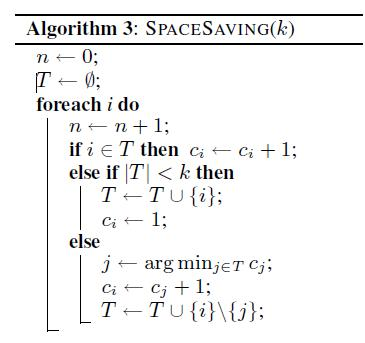
\includegraphics[width=12cm]{code_spaceSaving.jpg}
    \caption{Pseudo-code de l'algorithme SpaceSaving (Source : voir \cite{SpaceSaving2}) \label{fig:codeSpaceSaving}}
\end{figure}

\begin{figure}[H]
	\centering
        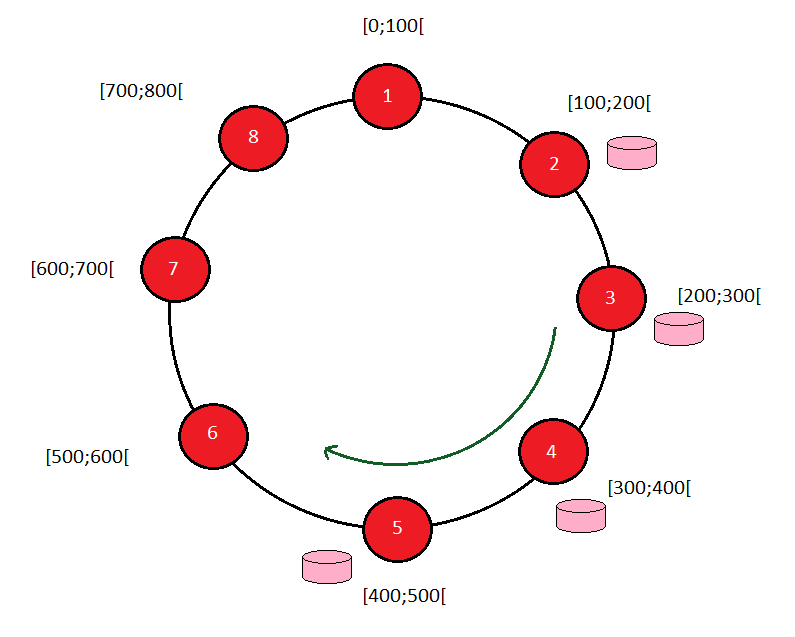
\includegraphics[width=12cm]{replication.png}
    \caption{Répartition des copies sur les noeuds dans une base de données distribuée \label{fig:replication}}
\end{figure}

\end{document}
